% Options for packages loaded elsewhere
\PassOptionsToPackage{unicode}{hyperref}
\PassOptionsToPackage{hyphens}{url}
\PassOptionsToPackage{dvipsnames,svgnames,x11names}{xcolor}
%
\documentclass[
  letterpaper,
  DIV=11,
  numbers=noendperiod]{scrreprt}

\usepackage{amsmath,amssymb}
\usepackage{iftex}
\ifPDFTeX
  \usepackage[T1]{fontenc}
  \usepackage[utf8]{inputenc}
  \usepackage{textcomp} % provide euro and other symbols
\else % if luatex or xetex
  \usepackage{unicode-math}
  \defaultfontfeatures{Scale=MatchLowercase}
  \defaultfontfeatures[\rmfamily]{Ligatures=TeX,Scale=1}
\fi
\usepackage{lmodern}
\ifPDFTeX\else  
    % xetex/luatex font selection
\fi
% Use upquote if available, for straight quotes in verbatim environments
\IfFileExists{upquote.sty}{\usepackage{upquote}}{}
\IfFileExists{microtype.sty}{% use microtype if available
  \usepackage[]{microtype}
  \UseMicrotypeSet[protrusion]{basicmath} % disable protrusion for tt fonts
}{}
\makeatletter
\@ifundefined{KOMAClassName}{% if non-KOMA class
  \IfFileExists{parskip.sty}{%
    \usepackage{parskip}
  }{% else
    \setlength{\parindent}{0pt}
    \setlength{\parskip}{6pt plus 2pt minus 1pt}}
}{% if KOMA class
  \KOMAoptions{parskip=half}}
\makeatother
\usepackage{xcolor}
\ifLuaTeX
  \usepackage{luacolor}
  \usepackage[soul]{lua-ul}
\else
  \usepackage{soul}
  
\fi
\setlength{\emergencystretch}{3em} % prevent overfull lines
\setcounter{secnumdepth}{5}
% Make \paragraph and \subparagraph free-standing
\ifx\paragraph\undefined\else
  \let\oldparagraph\paragraph
  \renewcommand{\paragraph}[1]{\oldparagraph{#1}\mbox{}}
\fi
\ifx\subparagraph\undefined\else
  \let\oldsubparagraph\subparagraph
  \renewcommand{\subparagraph}[1]{\oldsubparagraph{#1}\mbox{}}
\fi

\usepackage{color}
\usepackage{fancyvrb}
\newcommand{\VerbBar}{|}
\newcommand{\VERB}{\Verb[commandchars=\\\{\}]}
\DefineVerbatimEnvironment{Highlighting}{Verbatim}{commandchars=\\\{\}}
% Add ',fontsize=\small' for more characters per line
\usepackage{framed}
\definecolor{shadecolor}{RGB}{241,243,245}
\newenvironment{Shaded}{\begin{snugshade}}{\end{snugshade}}
\newcommand{\AlertTok}[1]{\textcolor[rgb]{0.68,0.00,0.00}{#1}}
\newcommand{\AnnotationTok}[1]{\textcolor[rgb]{0.37,0.37,0.37}{#1}}
\newcommand{\AttributeTok}[1]{\textcolor[rgb]{0.40,0.45,0.13}{#1}}
\newcommand{\BaseNTok}[1]{\textcolor[rgb]{0.68,0.00,0.00}{#1}}
\newcommand{\BuiltInTok}[1]{\textcolor[rgb]{0.00,0.23,0.31}{#1}}
\newcommand{\CharTok}[1]{\textcolor[rgb]{0.13,0.47,0.30}{#1}}
\newcommand{\CommentTok}[1]{\textcolor[rgb]{0.37,0.37,0.37}{#1}}
\newcommand{\CommentVarTok}[1]{\textcolor[rgb]{0.37,0.37,0.37}{\textit{#1}}}
\newcommand{\ConstantTok}[1]{\textcolor[rgb]{0.56,0.35,0.01}{#1}}
\newcommand{\ControlFlowTok}[1]{\textcolor[rgb]{0.00,0.23,0.31}{#1}}
\newcommand{\DataTypeTok}[1]{\textcolor[rgb]{0.68,0.00,0.00}{#1}}
\newcommand{\DecValTok}[1]{\textcolor[rgb]{0.68,0.00,0.00}{#1}}
\newcommand{\DocumentationTok}[1]{\textcolor[rgb]{0.37,0.37,0.37}{\textit{#1}}}
\newcommand{\ErrorTok}[1]{\textcolor[rgb]{0.68,0.00,0.00}{#1}}
\newcommand{\ExtensionTok}[1]{\textcolor[rgb]{0.00,0.23,0.31}{#1}}
\newcommand{\FloatTok}[1]{\textcolor[rgb]{0.68,0.00,0.00}{#1}}
\newcommand{\FunctionTok}[1]{\textcolor[rgb]{0.28,0.35,0.67}{#1}}
\newcommand{\ImportTok}[1]{\textcolor[rgb]{0.00,0.46,0.62}{#1}}
\newcommand{\InformationTok}[1]{\textcolor[rgb]{0.37,0.37,0.37}{#1}}
\newcommand{\KeywordTok}[1]{\textcolor[rgb]{0.00,0.23,0.31}{#1}}
\newcommand{\NormalTok}[1]{\textcolor[rgb]{0.00,0.23,0.31}{#1}}
\newcommand{\OperatorTok}[1]{\textcolor[rgb]{0.37,0.37,0.37}{#1}}
\newcommand{\OtherTok}[1]{\textcolor[rgb]{0.00,0.23,0.31}{#1}}
\newcommand{\PreprocessorTok}[1]{\textcolor[rgb]{0.68,0.00,0.00}{#1}}
\newcommand{\RegionMarkerTok}[1]{\textcolor[rgb]{0.00,0.23,0.31}{#1}}
\newcommand{\SpecialCharTok}[1]{\textcolor[rgb]{0.37,0.37,0.37}{#1}}
\newcommand{\SpecialStringTok}[1]{\textcolor[rgb]{0.13,0.47,0.30}{#1}}
\newcommand{\StringTok}[1]{\textcolor[rgb]{0.13,0.47,0.30}{#1}}
\newcommand{\VariableTok}[1]{\textcolor[rgb]{0.07,0.07,0.07}{#1}}
\newcommand{\VerbatimStringTok}[1]{\textcolor[rgb]{0.13,0.47,0.30}{#1}}
\newcommand{\WarningTok}[1]{\textcolor[rgb]{0.37,0.37,0.37}{\textit{#1}}}

\providecommand{\tightlist}{%
  \setlength{\itemsep}{0pt}\setlength{\parskip}{0pt}}\usepackage{longtable,booktabs,array}
\usepackage{calc} % for calculating minipage widths
% Correct order of tables after \paragraph or \subparagraph
\usepackage{etoolbox}
\makeatletter
\patchcmd\longtable{\par}{\if@noskipsec\mbox{}\fi\par}{}{}
\makeatother
% Allow footnotes in longtable head/foot
\IfFileExists{footnotehyper.sty}{\usepackage{footnotehyper}}{\usepackage{footnote}}
\makesavenoteenv{longtable}
\usepackage{graphicx}
\makeatletter
\def\maxwidth{\ifdim\Gin@nat@width>\linewidth\linewidth\else\Gin@nat@width\fi}
\def\maxheight{\ifdim\Gin@nat@height>\textheight\textheight\else\Gin@nat@height\fi}
\makeatother
% Scale images if necessary, so that they will not overflow the page
% margins by default, and it is still possible to overwrite the defaults
% using explicit options in \includegraphics[width, height, ...]{}
\setkeys{Gin}{width=\maxwidth,height=\maxheight,keepaspectratio}
% Set default figure placement to htbp
\makeatletter
\def\fps@figure{htbp}
\makeatother
% definitions for citeproc citations
\NewDocumentCommand\citeproctext{}{}
\NewDocumentCommand\citeproc{mm}{%
  \begingroup\def\citeproctext{#2}\cite{#1}\endgroup}
\makeatletter
 % allow citations to break across lines
 \let\@cite@ofmt\@firstofone
 % avoid brackets around text for \cite:
 \def\@biblabel#1{}
 \def\@cite#1#2{{#1\if@tempswa , #2\fi}}
\makeatother
\newlength{\cslhangindent}
\setlength{\cslhangindent}{1.5em}
\newlength{\csllabelwidth}
\setlength{\csllabelwidth}{3em}
\newenvironment{CSLReferences}[2] % #1 hanging-indent, #2 entry-spacing
 {\begin{list}{}{%
  \setlength{\itemindent}{0pt}
  \setlength{\leftmargin}{0pt}
  \setlength{\parsep}{0pt}
  % turn on hanging indent if param 1 is 1
  \ifodd #1
   \setlength{\leftmargin}{\cslhangindent}
   \setlength{\itemindent}{-1\cslhangindent}
  \fi
  % set entry spacing
  \setlength{\itemsep}{#2\baselineskip}}}
 {\end{list}}
\usepackage{calc}
\newcommand{\CSLBlock}[1]{\hfill\break\parbox[t]{\linewidth}{\strut\ignorespaces#1\strut}}
\newcommand{\CSLLeftMargin}[1]{\parbox[t]{\csllabelwidth}{\strut#1\strut}}
\newcommand{\CSLRightInline}[1]{\parbox[t]{\linewidth - \csllabelwidth}{\strut#1\strut}}
\newcommand{\CSLIndent}[1]{\hspace{\cslhangindent}#1}

\KOMAoption{captions}{tableheading}
\makeatletter
\@ifpackageloaded{bookmark}{}{\usepackage{bookmark}}
\makeatother
\makeatletter
\@ifpackageloaded{caption}{}{\usepackage{caption}}
\AtBeginDocument{%
\ifdefined\contentsname
  \renewcommand*\contentsname{Table of contents}
\else
  \newcommand\contentsname{Table of contents}
\fi
\ifdefined\listfigurename
  \renewcommand*\listfigurename{List of Figures}
\else
  \newcommand\listfigurename{List of Figures}
\fi
\ifdefined\listtablename
  \renewcommand*\listtablename{List of Tables}
\else
  \newcommand\listtablename{List of Tables}
\fi
\ifdefined\figurename
  \renewcommand*\figurename{Figure}
\else
  \newcommand\figurename{Figure}
\fi
\ifdefined\tablename
  \renewcommand*\tablename{Table}
\else
  \newcommand\tablename{Table}
\fi
}
\@ifpackageloaded{float}{}{\usepackage{float}}
\floatstyle{ruled}
\@ifundefined{c@chapter}{\newfloat{codelisting}{h}{lop}}{\newfloat{codelisting}{h}{lop}[chapter]}
\floatname{codelisting}{Listing}
\newcommand*\listoflistings{\listof{codelisting}{List of Listings}}
\makeatother
\makeatletter
\makeatother
\makeatletter
\@ifpackageloaded{caption}{}{\usepackage{caption}}
\@ifpackageloaded{subcaption}{}{\usepackage{subcaption}}
\makeatother
\ifLuaTeX
  \usepackage{selnolig}  % disable illegal ligatures
\fi
\usepackage{bookmark}

\IfFileExists{xurl.sty}{\usepackage{xurl}}{} % add URL line breaks if available
\urlstyle{same} % disable monospaced font for URLs
\hypersetup{
  pdftitle={CCESR Intern Hub},
  pdfauthor={CCESR Fellows},
  colorlinks=true,
  linkcolor={blue},
  filecolor={Maroon},
  citecolor={Blue},
  urlcolor={Blue},
  pdfcreator={LaTeX via pandoc}}

\title{CCESR Intern Hub}
\author{CCESR Fellows}
\date{}

\begin{document}
\maketitle

\renewcommand*\contentsname{Table of contents}
{
\hypersetup{linkcolor=}
\setcounter{tocdepth}{2}
\tableofcontents
}
\bookmarksetup{startatroot}

\chapter*{Welcome!}\label{welcome}
\addcontentsline{toc}{chapter}{Welcome!}

\markboth{Welcome!}{Welcome!}

This website / HTML book is intended to collect resources for Cedar
Creek summer interns doing independent research projects, and present
those resources in an easily accessible way.

For now, the focus is primarily on data management, analysis, and using
the R programming language.

Much of the content featured is adapted from the work of past CCESR
Fellows, including Maggie Anderson, Mariana Cárdenas, and Bea Baselga
Cervera.

This site is structured in different parts, which can be read in any
order you choose, depending on your needs / what you already know.
Currently, the first part describes data management practices, the
second part goes over data analysis in general, the third part describes
R-related software and workflows, and the fourth part is intended to
give a primer in R coding.

\part{Data Management}

\chapter{The Flow of Data}\label{the-flow-of-data}

In any scientific research, data management is a highly important skill.
As ecologists, we should strive to record, organize, document, and back
up our data in such a way that it will be accessible and useful to both
our future selves and other future researchers.

In general, the ``flow of data'' follows the this general pattern:

\begin{enumerate}
\def\labelenumi{\arabic{enumi}.}
\tightlist
\item
  ``Wild'' Data - these are our observations, features of the
  environment we wish to record as\ldots{}
\item
  Recorded Data - this is our first record of our observations, with
  which we ideally will\ldots{}

  \begin{enumerate}
  \def\labelenumii{\arabic{enumii}.}
  \tightlist
  \item
    Back Up - store copies in an alternative medium / location
  \item
    Error Check - look over the data for entry errors
  \item
    Other Processing - ensure proper filenames, data formats, etc.,
    leading to\ldots{}
  \end{enumerate}
\item
  Processed Data - this is the data that we can use to analyze and
  answer scientific questions!
\end{enumerate}

The following chapters will go into detail about this flow, with tips
and various things to consider.

\chapter{Recording Data}\label{recording-data}

First, let's go over how we can record ``wild'' data!

\section{Data Formats}\label{data-formats}

One thing to think about when recording your data is the formatting. In
data science, a commonly used dichotomy is between ``wide'' and ``long''
data formats. You are likely more used to wide data, but long data is
often better for scientific computing and analysis. Here is a
comparison:

\textbf{Wide Data}

\begin{itemize}
\item
  Easy for humans to read
\item
  Features unique rows for an identifier, with columns describing
  attributes
\end{itemize}

Example table of species abundance (attributes) at four research plots
(identifiers):

\begin{longtable}[]{@{}lll@{}}
\toprule\noalign{}
Plot & Species A & Species B \\
\midrule\noalign{}
\endhead
\bottomrule\noalign{}
\endlastfoot
North & 3 & 3 \\
East & 0 & 3 \\
South & 1 & 0 \\
West & 2 & 0 \\
\end{longtable}

\textbf{Long Data}

\begin{itemize}
\item
  Easy for computers to read
\item
  Features multiple rows for each identifier value, one for each
  attribute
\end{itemize}

Example table of the same data from above:

\begin{longtable}[]{@{}lll@{}}
\toprule\noalign{}
Plot & Species & Count \\
\midrule\noalign{}
\endhead
\bottomrule\noalign{}
\endlastfoot
North & A & 3 \\
North & B & 3 \\
East & A & 0 \\
East & B & 3 \\
South & A & 1 \\
South & B & 0 \\
West & A & 2 \\
West & B & 0 \\
\end{longtable}

As you can see, long data take more space, but it is easier to select
and compare data in a computing environment when it is in this format.
You will see this in action in the R programming section of this
website!

\section{Data Sheet Design}\label{data-sheet-design}

Whether you design a data sheet using long or wide format, you will need
to use some sort of computer application, either a spreadsheet program,
word processor, or a combination of both. You are probably familiar with
many of the options, but here are a few -

\textbf{Spreadsheet Applications:}

\begin{itemize}
\item
  Microsoft Excel - Standalone program, often free with university
  accounts
\item
  Google Sheets - web-based, free to use with Google account, can be
  integrated directly with R
\item
  LibreOffice Calc - Standalone program, free and open-source
  alternative to Excel
\end{itemize}

\textbf{Word Processors:}

\begin{itemize}
\item
  Microsoft Word - Standalone program, often free with university
  accounts
\item
  Google Docs - web-based, free to use with Google account
\item
  LibreOffice Writer - Standalone program, free and open-source
  alternative to Word
\end{itemize}

Sometimes it can be finicky to design a data sheet directly in a word
processor's table functionality. Instead, you can create the basics of
your table in a spreadsheet application, and then copy and paste it into
the word processor, and then fine-tune the table to your liking.

When designing your sheet/s, wide data will often be more intuitive and
easier for recording, but note that there may be more processing steps
required when you get to the analysis stage (and if the data are
complex, the data manipulation required can also be complicated). On the
other hand, recording data in long format, while somewhat tedious, will
be efficient for later processing and analysis steps.

In general, wide format for recording data is effective for simple
observations when you know exactly how much you are going to record
(e.g., a suite of soil attributes for a set of plots). Long format can
be effective when the observations you're recording are more complicated
and/or you don't know how many observations you will be making in a
given plot (e.g., recording each plant species with it's cover class,
max height, and disease severity in a set of plots - you might not know
how many species you will encounter in each plot!).

\textbf{Universal Tip:} Always include a ``Notes'' column!

\section{Data Sheet Medium}\label{data-sheet-medium}

When it comes to recording data in the field or in the lab, there are
two main styles: using paper data sheets or using electronic
spreadsheets/apps. Opinions vary among researchers.

\textbf{Paper / Physical Media}

\begin{itemize}
\item
  Traditional method for ecology research
\item
  Results in having both a hard copy and electronic copy of the data

  \begin{itemize}
  \tightlist
  \item
    Backups can include photos/scans of the paper data sheets, as well
    as back-up electronic files
  \end{itemize}
\item
  Less risk of technical glitches
\item
  Need to consider material; write-in-the-rain and pancil often
  necessary in field settings
\item
  Needs a solid organization scheme to make sure paper sheets don't get
  lost or misplaced
\item
  Requires data to be entered from paper to computer

  \begin{itemize}
  \tightlist
  \item
    But this does leave the chance for checking for entry errors between
    paper and computer
  \end{itemize}
\end{itemize}

\textbf{Electronic Media / App-based Recording}

\begin{itemize}
\item
  Becoming more popular among large-scale projects (e.g., National
  Ecological Observatory Network)
\item
  Some projects use propietary software for data recording, but you can
  use the Google Sheets app
\item
  Data is usually only digital files, but can be printed out for hard
  copy back-ups
\item
  Somewhat elevated risk for technical glitches / user error
\item
  Can utilize immediate cloud backup
\item
  Phone data entry can be particularly convenient for certain field
  methods
\item
  Error checking is limited to looking for obvious field entry errors
  (e.g., impossible attribute values)
\end{itemize}

\chapter{File Organization}\label{file-organization}

As our recorded data moves into electronic form, either directly from
our field/lab observations or via data entry from paper data sheets, it
is important to consider how we organize and name our electronic files.
It may sound boring, but it is valuable to think about!

\textbf{Universal Tip:} Be consistent!

\section{Organize}\label{organize}

When you are developing an organization scheme, there are many ways you
can proceed. Here are a few:

\textbf{File Organization Strategies}

\begin{itemize}
\item
  By Stage - collection materials, raw data, processed data, shared
  data, etc.
\item
  By Data Type - text, images, spreadsheets, etc.
\item
  By Research Activities - experiments, field observations, interviews,
  etc.
\end{itemize}

The best way to organize your files will depend on the project and the
researcher, but as long as it is consistent, it is effective.

The strategies listed above generally work best as coarse-scale
organization schemes, but one strategy could be used as a subfolder
scheme within another strategy.

Date and location generally work best as subfolder organization schemes
within one of the above strategies. One exception to this might be when
you are doing radically different things among years or locations.

When you are downloading research related files, it is best to move them
from the ``downloads'' folder as soon as possible, or better yet,
download directly to the appropriate folder and subfolder. And avoiding
downloading important files to the desktop is generally helpful.

Finally, Do not use your folders as the sole description of your files,
i.e., use descriptive file names! A file named ``plot3'' may make sense
in your ``2023\_BioCON'' folder, but it will lose context when moved or
shared. This brings us to our next section\ldots{}

\section{Name}\label{name}

Descriptive file names should be easily scannable and sortable.

Key components of a descriptive file name often include:

\begin{itemize}
\item
  Project name
\item
  Date (YYYYMMDD)
\item
  Type of data
\item
  Location/site
\item
  Researcher Info
\item
  Version
\end{itemize}

For sorting purposes, it is best to use numerical date format and
leading zeroes. Numerical date format is YYYYMMDD, or 20240710 instead
of something like 7-10-24. When sorted, everything will be in calendar
order. Sorting other date formats can lead to files being out of order,
like how 12 comes before 7 in an alphanumeric sort, so December could
come before July in your files. Similarly, since 10, 11, 12, etc. come
before 2 in an alphanumeric sort, it is good to use leading zeroes
depending on the number of numeric IDs you have. For example if you have
12 plots, use one leading zero for plots 1-9 to ensure proper file
sorting (e.g., ``01'', ``02'', etc.).

\textbf{Universal Tips:}

\begin{itemize}
\item
  Don't use special characters (*@,.\^{}?\#!\textless\textgreater)

  \begin{itemize}
  \tightlist
  \item
    These are incompatible with many file systems
  \end{itemize}
\item
  Be concise, AKA brief but efficiently informative
\end{itemize}

\chapter{Documentation and Storage}\label{documentation-and-storage}

``Your primary collaborator is yourself 6 months from now \& your past
self doesn't answer email!''\\
\strut \\
- Rachel Ainsworth

Taking notes as you conduct research and backing things up are both
generally good practice. Here are some things to think about regarding
both:

\section{Document}\label{document}

\textbf{What} \textbf{to document:}

\begin{itemize}
\item
  File-specific info or metadata

  \begin{itemize}
  \item
    file naming patterns
  \item
    variable/attribute definitions
  \end{itemize}
\item
  Technical steps

  \begin{itemize}
  \item
    data collection
  \item
    processing (what did you include or exclude?)
  \item
    analysis steps
  \end{itemize}
\item
  External data sources
\item
  Software used with version numbers
\item
  Meeting notes
\item
  Organization schemes
\end{itemize}

\textbf{Where to document:}

\begin{itemize}
\item
  Lab Notebook

  \begin{itemize}
  \item
    Can be physical or digital
  \item
    Many scientists use pen for this sort of thing
  \end{itemize}
\item
  Field notebook

  \begin{itemize}
  \tightlist
  \item
    Generally easier to be physical if taking notes in the field, can be
    digital if taking notes at end of day
  \end{itemize}
\item
  ReadMe file

  \begin{itemize}
  \tightlist
  \item
    Good for computer work - data processing and analysis
  \end{itemize}
\end{itemize}

\textbf{When to document:}

\begin{itemize}
\item
  Set aside \textasciitilde15 minutes after your work session
\item
  Develop a regular routine during the research process

  \begin{itemize}
  \tightlist
  \item
    Easier to do than remembering everything at the end
  \end{itemize}
\item
  Can also note things opportunistically as you go

  \begin{itemize}
  \item
    jot potentially relevant observations down in a notebook
  \item
    comment out code
  \end{itemize}
\end{itemize}

\section{Store}\label{store}

The methods of backing up your data may vary somewhat based on medium,
but what remains important universally is to maintain multiple formats
of backups, and it is helpful to have one backup in an alternative
physical location.

\textbf{Paper Data Sheets}

\begin{itemize}
\item
  take a photo or scan each newly filled data sheet after each day of
  data collection
\item
  Back up entered data files in cloud storage or some other location
\end{itemize}

\textbf{Electronic Data}

\begin{itemize}
\item
  Download a dated copy of all electronically entered files after each
  day of data collection

  \begin{itemize}
  \tightlist
  \item
    You can write an R script to do this for you with Google Sheets
  \end{itemize}
\end{itemize}

You may also run into some issues when storing backups. You may run out
of storage space, especially on personal cloud storage accounts.
However, usually university or organization based accounts have large
storage limits. In addition, physical data drives (either hard drives or
solid-state drives) can fail, so it's good to have cloud-based storage
and/or alternate physical drives (another computer or external drive) as
fail-safes. Of course, cloud storage providers can change terms in the
near future, so be prepared for adapting your plans.

\chapter{Error Checking and Data
Processing}\label{error-checking-and-data-processing}

Finally, when you have your data recorded, organized, documented, and
backed-up, there are a few things to think about before analysis:
checking for errors and late-stage processing steps.

\section{Error Checking}\label{error-checking}

Your error checking method may vary depending on the medium on which
your data were recorded, but a general note is that you can elect to
error check everything, or a certain percentage of all the data when
data are numerous. Different organizations will follow different
practices. Oftentimes personal research projects are small scale enough
that full error checking is feasible.

\textbf{Paper Data}

\begin{itemize}
\item
  Cross reference digitally entered data with paper sheet for errors in
  entry

  \begin{itemize}
  \tightlist
  \item
    Helpful to have two people
  \end{itemize}
\item
  Note any corrections in a new column
\item
  Hard to check field recording errors, but make any corrections in a
  different colored writing utensil for clarity
\end{itemize}

\textbf{Electronic Data}

\begin{itemize}
\item
  Check version control (e.g., Google Drive files) for unusual edits,
  and roll back where necessary

  \begin{itemize}
  \tightlist
  \item
    Note when you rolled back a change in a new column
  \end{itemize}
\end{itemize}

\section{Data Processing}\label{data-processing}

When you are getting ready to analyze your data, the best file formats
are text-based with some sort of delimiter between columns.

The most popular of these file formats is the ``comma separated value''
file, or .csv. It is small in size, as it is a simple text file where
commas denote new columns and line breaks denote new rows. This is easy
for a wide variety of computer programs to interpret, and will most
likely continue to be efficient for the foreseeable future.

Unlike Excel spreadsheets or Google Sheets, text based format do not
support multiple sheets, cell/text colors, or special formatting. As
such, do not rely on color or font for describing your electronic data.

You can create .csv files form Excel using the ``Save as'' command and
selecting the csv format, and you can download a Google Sheet as a csv
as one of the options. You can also ``publish'' a Google sheet as a csv
on the web to import directly into R, but that is a topic for later in
this site (see \hyperref[sec-web_import]{15.1.3 Importing Data; From the
Web})

\part{Data Analysis}

\chapter{Data Analysis at a Glance}\label{data-analysis-at-a-glance}

Analyzing your data is usually about transforming long spreadsheets into
a form that is relevant to your question/s, and oftentimes including an
appropriate statistical approach for inference.

You might use \textbf{descriptive statistics}, which is simply
\emph{describing} what you observed without presenting every data point,
and instead a summary of those data. This can often be helpful in
providing a frame of reference to your dataset before looking deeper at
trends and comparisons. Alternatively, sometimes descriptive statistics
are the main goal - like in surveys of populations and communities
(e.g., what is the population size of a certain grass of interest in an
old field?). Descriptive statistics include things like the mean and
variance, but can also include less commonly used measures like
dispersion (which is simply the variance : mean ratio!).

You could also use \textbf{inferential statistics}, which is more about
using math or simulation techniques to \emph{infer} some conclusion from
the shape of your data. This is directly relevant to when you have an
ecological question about cause and effect, associations among
variables, comparisons among categories, etc. The results of inferential
statistics provide a starting point from which to interpret/discuss an
answer to your question. Examples include t-tests and linear regression.

When using both of these types of statistics, you should be mindful of
\textbf{data types}, which are the form that variables take. For
example, the height of a tree is number, but the species of a tree is a
category. This contrast is obvious, but there are subtle differences
that can be important for how you describe, assess, and plot your data.
We will go over data types in the very next section!

\chapter{Data Types}\label{data-types}

As mentioned in the last section, we will now go over different types of
data:

\section{Numeric Data}\label{numeric-data}

Any data that can be described with numbers or have quantifiable
relationships between values is numeric. But! There are multiple types
of numeric data. The most important distinction is \textbf{discrete} vs
\textbf{continuous}.

\textbf{Discrete} numeric data is data where not every value is
possible, but you can still quantify specific differences among the
possible values - the major example being integer values (1, 2, 3, the
rest). Most programming languages will refer to this type as ``integer''
or ``int''. Examples might include number of ants on a log.

\textbf{Continuous} numeric data is data where every value is possible!
So this is basically all real numbers, including decimals (1.0, 1.1,
etc.). Many programming languages will refer to this as simply numeric
data, but lower level languages might use ``float'' or ``double''.
Examples might include the biomass of ants on a log. Note: measures that
consist of very large integer values (e.g., when you get up to 4 digits)
are approximately continuous.

Other things to consider with numeric data is whether the scale of
measurement is bound by any values. For example, the number of or
biomass of ants on a log cannot be less than zero. In addition,
percentages and proportions are bound by 0 and 100 and 0 and 1
respectively. These limitations can lead to special considerations when
performing inferential statistics.

\section{Categorical Data}\label{categorical-data}

Any data for which the values have no specifically quantitative
difference among them is categorical. Again there is one majorly
important distinction: \textbf{nominal} vs \textbf{ordinal}.

\textbf{Nominal} data is data where categories have no ranking or order,
like the species of ants on a log.

\textbf{Ordinal} data is data where categories have some order, like
your top 5 favorite breakfast cereals. But wait! You may be thinking -
``isn't this quantitative?'' Well yes and no. The difference between
ordinal data and discrete numeric data is that you can't really quantify
the exact difference between ordinal data values. Say there is a go-kart
race between Mario, Luigi, and Peach. The place that each finished would
be ordinal, e.g., Peach got 1st and Luigi 2nd, but you wouldn't be able
to say how much faster Peach was than Luigi. The time it took for Peach
and Luigi each to finish the race would be a numeric variable, and there
would be a specific value difference between them.

\chapter{Descriptive Statistics}\label{descriptive-statistics}

Now, let's discuss how to describe your data:

\section{Centrality}\label{centrality}

You'll often want to describe the central tendency of your data - around
where are the values centered?

\textbf{Mean} - the average of the values, or the sum of all values
divided by the number of observations

\textbf{Median} - the value at which half of the observations are
greater, and the other half are less

\textbf{Mode} - the most commonly observed value

Usually, the mean is a perfectly adequate descriptor. You can use it on
continuous numeric data, discrete numeric data (though the mean value
will often be unrealistic), or even ordinal rankings.

\textbf{When might you prefer to use the median over the mean?}

When the data is skewed such that there are many small values and a few
big values, the mean might be inflated by those large values, and thus
overestimate the central tendency in some contexts.

When data is roughly normally distributed, the mean and median are
roughly the same:

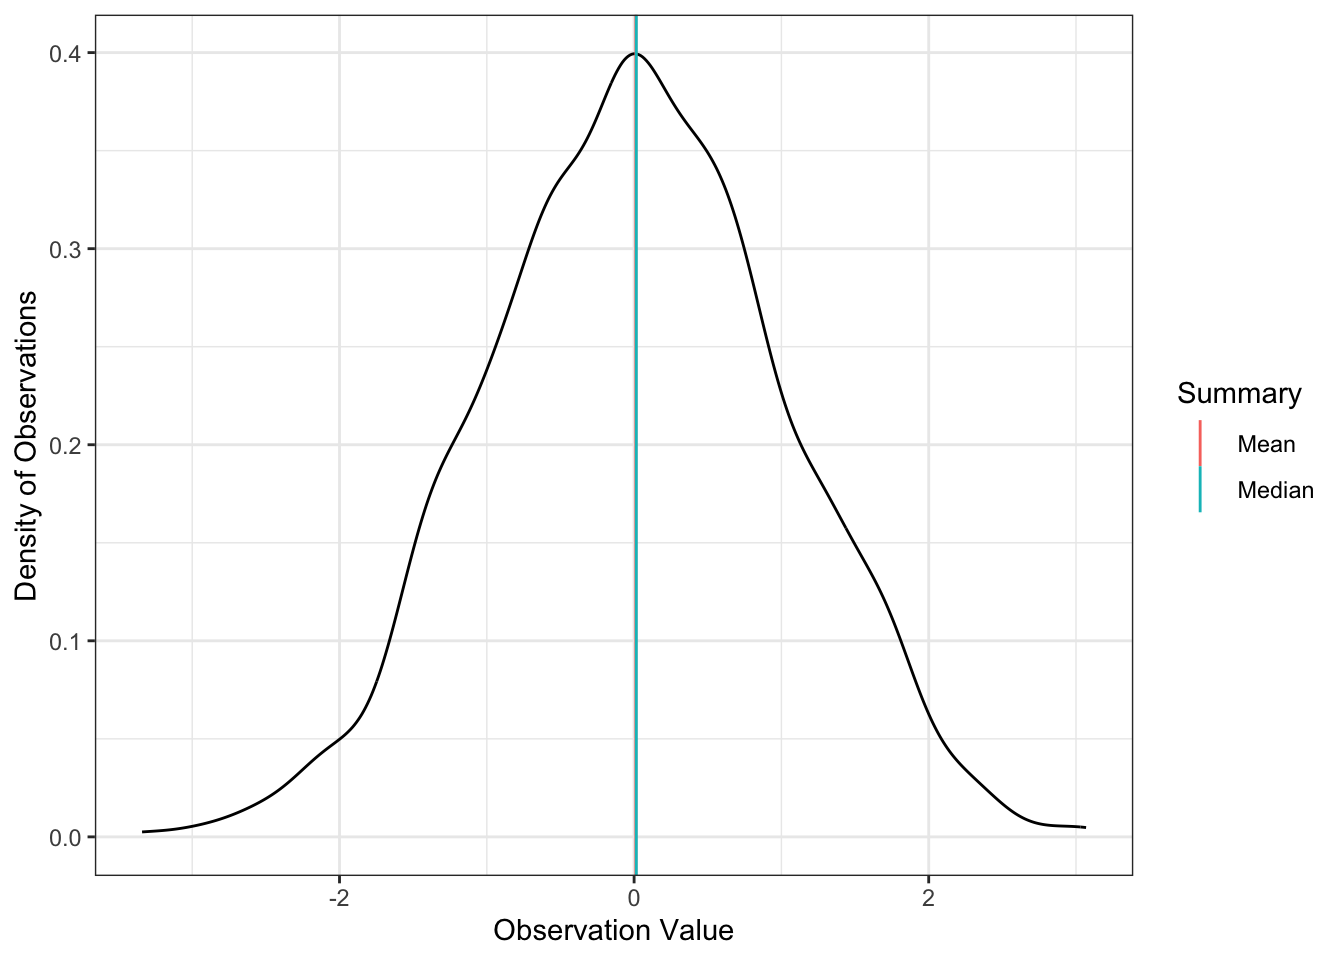
\includegraphics{da_describe_files/figure-pdf/unnamed-chunk-1-1.pdf}

But when data are skewed, the median may be a better estimate of the
central tendency:

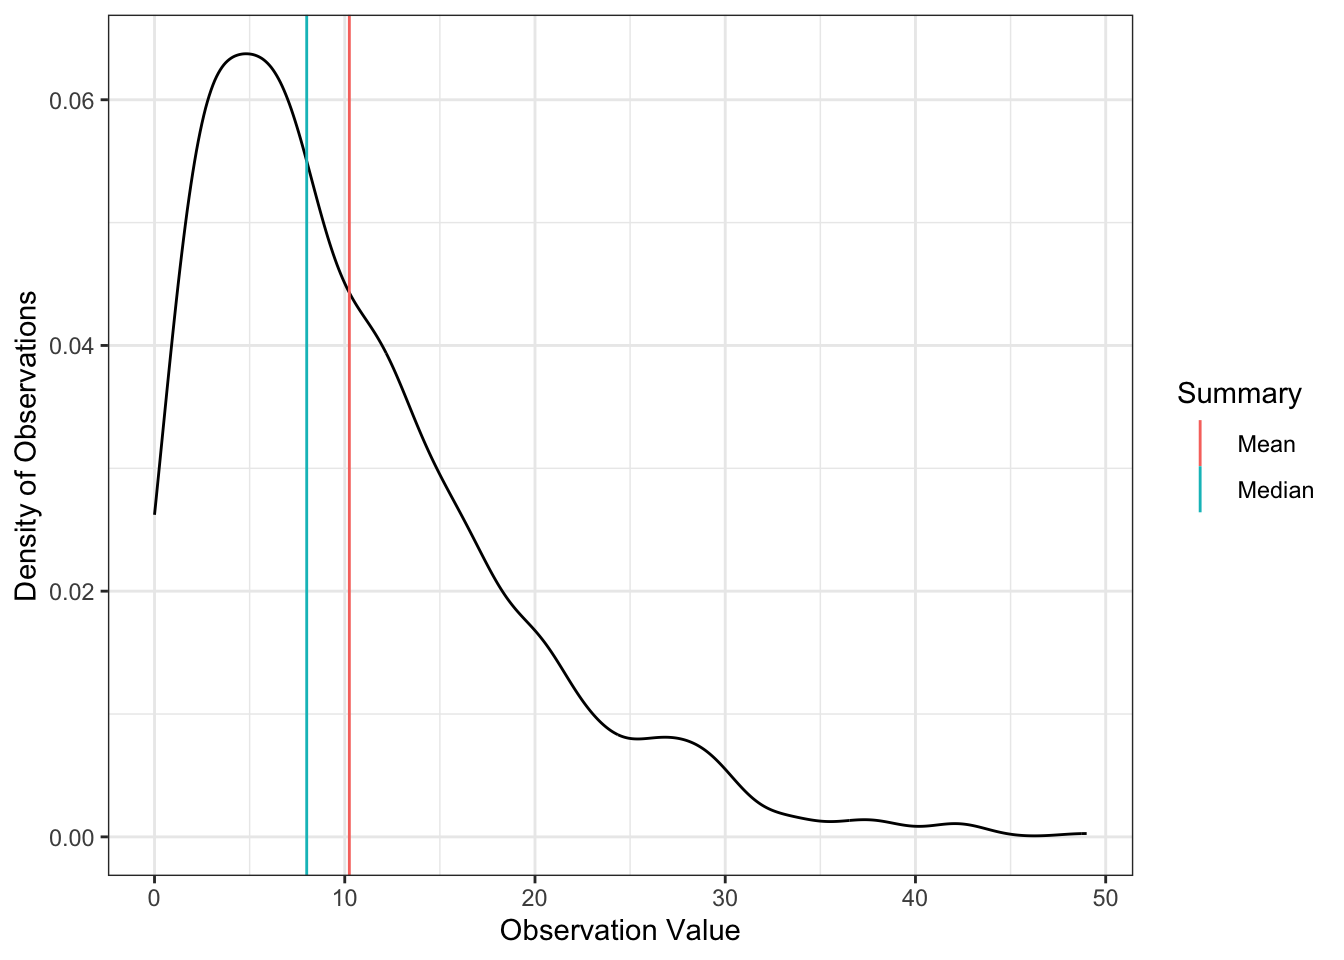
\includegraphics{da_describe_files/figure-pdf/unnamed-chunk-2-1.pdf}

\section{Spread}\label{spread}

You also might be interested in how varied your data is, how much it
deviates from the central tendency. This can be done with the following:

\textbf{Variance} - how variable is the data? Measured as the average
squared difference between observations and the mean:

\[
Variance = \frac{\sum (Observation_i - Mean)^2}{Number of Observations}
\]

(\(\sum\) means ``sum of'')

The differences are squared to get rid of negative differences, because
other wise everything would cancel out and our variance would be zero!

\textbf{Standard Deviation} - the square root of the variance. This is
useful because it is in the same units as the original measurements!

\section{Other Descriptors}\label{other-descriptors}

Another descriptor that may prove useful is the \textbf{dispersion}, or
the variance divided by the mean. This provides an estimate of how
skewed the data is - for example, the first plot above has very low
dispersion, while the second plot has high dispersion.

\section{Ecological Community
Descriptors}\label{ecological-community-descriptors}

Many of you are interested in describing the species composition of of
community. Here's a few common descriptors:

\textbf{Species Richness} - this is just the number of different species
present.

\textbf{Species Diversity} - this is an index that takes into account
the richness as well as the relative abundances of each species. E.g.
Shannon's Diversity Index, where higher numbers mean more species more
evenly distributed.

\textbf{Species Evenness} - this is an index that estimates specifically
how evenly distributed species abundances are. E.g., Pielou's Evenness,
which ranges from 0 to 1, with 1 meaning that each species has equal
numbers.

Note: these measures can apply to any taxonomic distinction, e.g.,
family richness, order diversity, etc.

\chapter{Inferential Statistics}\label{inferential-statistics}

Now, let's think about how to use your data to answer your questions.
There are a couple of approaches statisticians use, and we will talk
about frequentist statistics, where probabilities are thought of like
relative frequencies. There is also Bayesian statistics, which is a bit
more complex, so we will skip it for now.

Within frequentist statistics, we can run various tests to see how
variables are related, which typically make some assumptions about the
data. We can also do something called bootstrapping, which makes no
assumptions, but can be simplistic from some perspectives.

In any case, we are hoping to estimate two main values:

\textbf{Effect Size}: How related are two variables? How different are
two means? How much does one variable affect another?

\textbf{p-value}: What is the chance of observing data like yours (or
something more extreme) if there was no relationship among the
variables?

The p-value can be a bit tricky, but know that it \textbf{isn't} the
probability that there is no relationship. P-values are used to draw
conclusions from test results, a traditional guideline is that if the
p-value is less than 0.05, the results are ``significant.'' Some
statisticians bristle at this arbitrary and binary system, so it's often
best to report both the effect size and the actual p-value, so readers
can interpret for themselves. The smaller the effect size, the weaker
the relationship, the smaller the p-value, the stronger the evidence for
the relationship.

Obviously, there are entire classes taught on this stuff (which many of
you may have taken or will take!), but we are thinking in just the
basics for now.

\section{Classic Frequentist Tests}\label{classic-frequentist-tests}

Now let's go over some statistical tests! For this section, it can be
useful to remind ourselves of the variables involved in a research
question:

\textbf{Independent / Explanatory / Predictor Variable}: this is either
what you are manipulating in an experiment or what your study is
designed to capture variation in (e.g., C02 at BioCON, species richness
at BigBio).

\textbf{Dependent / Response Variable}: these are what you measure or
observe throughout your study, generally hypothesizing that they will
differ among the levels of your independent variable (e.g., aboveground
biomass in BioCON or BigBio).

\subsection{Assumptions}\label{assumptions}

We should mention what these tests generally assume about your data.

First, they assume that your \textbf{data are independent}. This just
means that no two observations of your data are more related to each
other in a way that isn't accounted for by a variable. Say you were
comparing mean tree height between two forests - individual tree heights
in the same forest would be independent, but two measures of the same
tree on different days would be non-independent.

Second, they assume that the \textbf{errors are normally distributed}.
This is a bit more confusing without a statistical background. An
example may be illustrative - in the tree height example above, we
assume that the individual tree heights are normally distributed around
the mean. Without getting too much into the weeds, if you collect enough
data (i.e., 30+ observations), these errors will likely be approximately
normally distributed. However, things get dicey when we deal with data
that is not continuous like tree height, for example, discrete count
data - more on that below.

Third, they assume \textbf{homogeneity of variance}. This is another
complicated one, but it mean that the variance of the errors doesn't
change with the independent variable. In the tree example, we are
assuming that the variance of the differences between observed tree
heights and the forest mean does not change between forests.

Data that break the first assumption are difficult to deal with outside
of accounting for the non-independence factor (which can severely reduce
the size of your sample), but failing to meet the second or third
assumptions generally leads to transforming data or using alternative
tests.

\subsection{Categorical Predictor/s, Numeric
Response}\label{categorical-predictors-numeric-response}

\subsubsection{Two Predictor Categories}\label{sec-ttest}

When you are comparing numeric values from two groups, you can use a
\textbf{t-test} to compare their means. T-tests can be \textbf{paired}
when each observation in one group is specifically linked to an
observation in the other group (e.g., masses of sibling plants in
separate treatments) which can be more powerful. When the variance of
values in each group is different, you can do a \textbf{t-test with
unequal variance}.

The effect size here is the difference between means.

\subsubsection{More Than Two Predictor Categories}\label{sec-anova}

If you have more than two groups/categories, you can use a
\textbf{Analysis of Variance} or \textbf{ANOVA}. This will tell you if
the means of each group are equivalent, or if there is at least one
inequality. You can test for pairwise comparisons among the groups with
\textbf{Tukey's test}. If you have multiple categorical predictors, you
can do \textbf{two-way or three-way ANOVAs}. Tests with more than three
categorical predictor variables are uncommon and harder to interpret.

The effect sizes are the pairwise difference in means.

\subsubsection{Ordinal Predictors}\label{ordinal-predictors}

When your predictor variable is ordinal, the quick and easy way to
analyze it would be to convert the predictor to a numeric integer data
type and proceed from there. However this is imprecise\ldots{}

\emph{This section is under construction}

\subsection{Numeric Predictor/s, Numeric
Response}\label{numeric-predictors-numeric-response}

\subsubsection{Simple Association}\label{sec-corr}

When all you are interested in is whether two numeric variables are
related to one another, not cause and effect, you can do a
\textbf{correlation test}. \textbf{Pearson's correlation} is generally
applicable for continuous data. \textbf{Spearman's correlation} is good
for when you are dealing with data with non-normal distributions, like
count data (it also works for ordinal data!).

The effect size here will be a correlation coefficient ranging from -1
to 1, with -1 means an inverse relationship, 0 means no relationship,
and 1 mean a direct positive relationship.

\subsubsection{Cause and Effect}\label{sec-reg}

When you are suppose a causal relationship between numeric variables,
you can use a \textbf{linear regression}. This will use linear algebra
or maximum likelihood estimation (don't worry about the finer details
here) to find the best fit line that describes the relationship between
two variables; where the sum of the squared distances from the
observations to the line is minimized. You can also include multiple
predictor variables to perform \textbf{multiple linear regression} AKA
\textbf{multivariate linear regression}.

When your response variable is count data, the assumptions of simple
linear regression are usually unmet, so you can use generalized forms
like a \textbf{Poisson regression} or a \textbf{Negative Binomial
regression}.

The effect sizes here are the parameter coefficients, i.e., how much
does the response change for on unit increase in the predictor? Note:
these are not straightforward for Poisson and negative binomial
regression, so ask your mentor.

\subsection{Numeric Predictor/s, Categorical
Response}\label{numeric-predictors-categorical-response}

\subsubsection{Binary Response}\label{sec-bin}

When your categorical response is only two categories (e.g., presence or
absence), you can use a \textbf{binomial regression} AKA
\textbf{logistic regression}. This works similarly to linear regression,
but the effect sizes are measured in log odds, which is difficult to
interpret, but can be transformed to estimating how the probability of
observing one category value instead of the other increases with a
variable.

\subsubsection{Multiple Response
Categories}\label{multiple-response-categories}

\textbf{Multinomial regression} \emph{(under construction)}

\subsection{Categorical Predictor/s, Categorical
Response}\label{categorical-predictors-categorical-response}

\textbf{Chi-square test} \emph{(under construction)}

\section{Bootstrapping}\label{bootstrapping}

One alternative to these classic tests has no assumptions:
bootstrapping. Essentially, it involves using the sampled data to
simulate more samples, and compare your observations to those
simulations.

\textbf{Empirical Bootstrapping} is where you take your actual
observations and shuffle which value is associated with which
observation. For example, you could take measurements of tree heights
from two forests, and randomly assign forest ID to each measurement.

\textbf{Parametric Bootstrapping} is where you summarize your observed
data and use it to generate simulated data. For example, you could
calculate the mean and variance of tree heights in two forests and then
generate simulated forests of trees through random pulls from a normal
distribution with the appropriate mean and variance.

With both approaches, you simulate a large number of simulated datasets
(1000+), and then calculate whatever you are interested in for each of
those simulations, and compare the calculation from the observed data to
the distribution of simulated values. For example, if you empirically
bootstrap the two forests of tree heights 1000 times, and then calculate
difference in means for each you will have 1000 mean difference values.
The proportion of those simulated values that are equal to or more
extreme than your observed mean difference is your p-value!

\part{R on your Computer}

\chapter{R Itself}\label{r-itself}

R is both a programming language and an application that you can install
to your computer.

\section{R, the Language}\label{r-the-language}

R is a programming language designed for statistical computing, and is
often the language of choice for scientists. R is also used for data
science in some business, tech, and health contexts (but many prefer
Python in those areas).

As a programming language it is essentially an expandable collection of
functions with syntax to perform tasks, and it could be written in any
text editor. However, in order for your computer to interpret the
language, it needs some software.

\section{R, the Software}\label{r-the-software}

The R application allows you to run R code on your computer, and comes
with a basic ``console'' window where code is run and output is printed,
as well as a basic script editor where you can write code to run.

You can download the application from here:

\url{https://cran.r-project.org/}

If you are asked to select a mirror, simply select the nearest one (I
believe Iowa State should work).

If you have a Windows machine, it should be fairly straightforward to
simply download and install the ``base'' R from the link.

If you have a Mac, you will want to select the .pkg file that matches
your processor type: x-86 for Intel processors (mostly Macs pre-2020),
arm64 for Macs with the M1 or M2 chip (most Macs post-2020).

If you are using Linux, you know more than me.

\section{R Packages}\label{r-packages}

As mentioned above, R is \emph{expandable}. You can add more
functionality to R by installing packages. Packages contain more options
of code to use to process and analyze data, and also do many other
things.

Packages can be installed through writing R code, or by clicking some
buttons in RStudio. Then they will live in a directory that was built
when you installed R for auxiliary packages.

We will discuss more about installing packages in the R coding section.

\chapter{R Studio}\label{r-studio}

While you can use R with just the basic application, it is much easier
and beginner-friendly to use RStudio, which is an integrated development
environment or IDE. This is just an application that provides a suite of
features to make programming easier for users. In fact, I'm typing this
in RStudio \emph{right now}!! Note: you must have the R application
installed to use RStudio, as it relies on the R application to interpret
R code.

You can download and install RStudio from here:

\url{https://posit.co/download/rstudio-desktop/}

Which should be more straightforward than downloading and installing R.

\section{RStudio at a Glance}\label{rstudio-at-a-glance}

If you open up RStudio, you will see something like this:

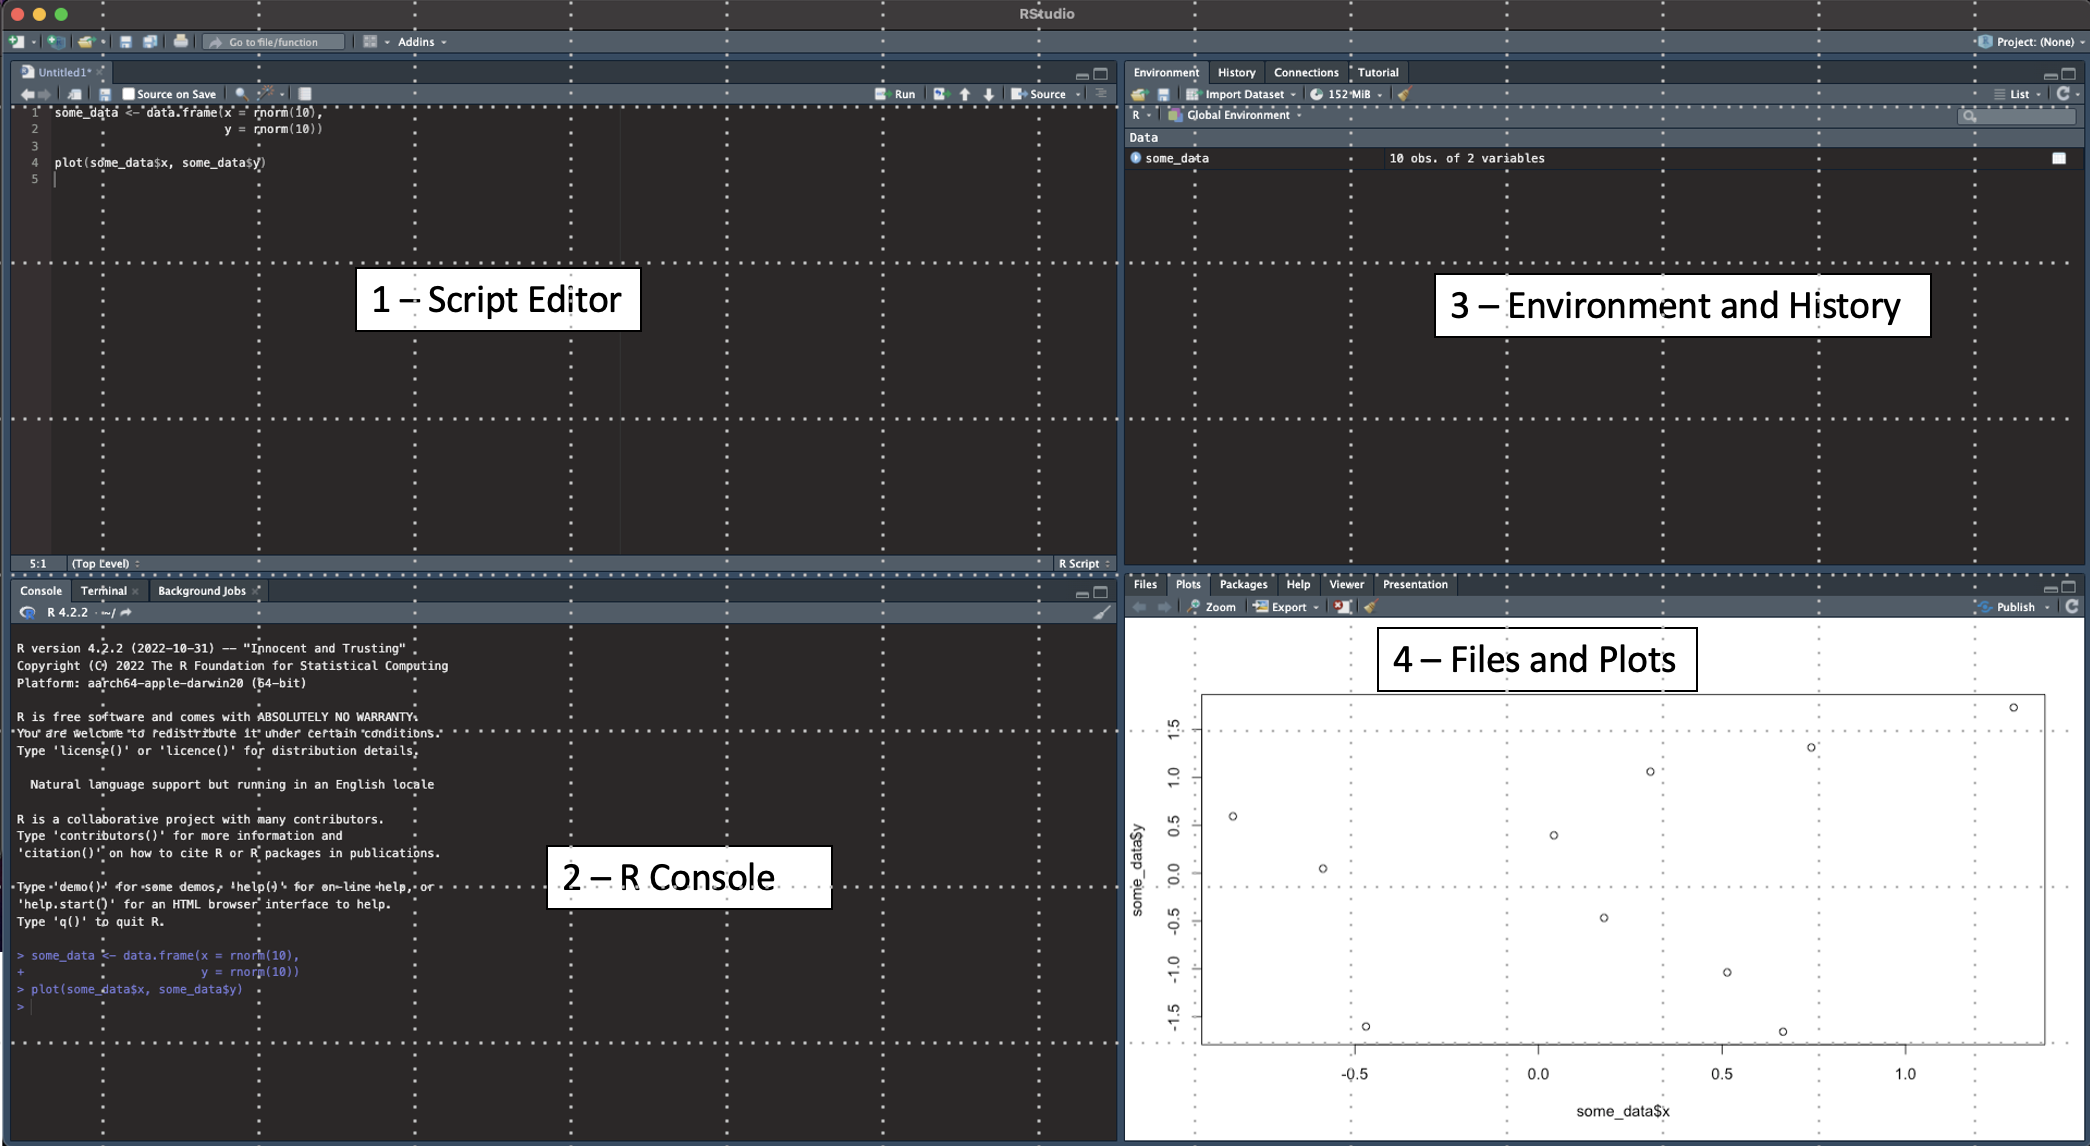
\includegraphics{rstudiowindow.png}

\textbf{1- Script Editor}: Here is where you will write code! You can
create an R script (a text document to save code in) with the file tab,
and write what you need in the resulting script. It is \textbf{highly}
recommended to use scripts, because then you can save your code for
later, and troubleshoot errors easier. From this window, you can
highlight code and run it with the ``Run'' button on top, or with Ctrl +
Enter / Cmd +Enter.

\textbf{2- R Console}: Here is where the action happens - code will run
here, and text output, warnings and messages will be displayed. You can
also type code into the console, but that is only recommended for
installing packages, entering credentials, rendering documents, and
things of that nature. Don't type your data processing or analysis code
into the console, use a script instead! There's also a terminal tab if
you ever need to perform shell commands (which is probably unlikely for
your project this summer).

\textbf{3- Environment and History}: Here you can find a list of the
variables and data you have loaded into your ``workspace'' or
``environment'' in the Environment tab. These are objects you can do
stuff with with code. You can also click the History tab to see the code
you have run thus far.

\textbf{4- Files and Plots}: Here is where any figures you draw will pop
up (and you can save them from here as well). There is also a Files tab
that allows you to navigate through your file directory (helpful with
projects, described below). The Packages tab shows which packages you
have installed and loaded (you can also click ``Install'' at top to
easily install new ones!). Finally, the help tab is where you can search
for the documentation on any R function.

\section{R Projects}\label{sec-rprojects}

It is highly recommended to use R Projects when working with RStudio.
Projects are essentially just subdirectories in your file folders, but
they come with a special .Rproj file that RStudio can read and use. This
helps you organize your work, and makes your code more easily portable.

You can create a new projects from the File tab at upper left, or in the
project dropdown menu at upper right. You can just create one in a new
directory. Then you can select a name and where you want to save it.

There are many different types of projects - this book/website is one!

If you want to backup your work with version control or collaborate with
others using git and GitHub, you will need to use projects. (Well,
technically you don't need to, but you'd be doing many things manually).

\chapter{Optional: Git and Github}\label{optional-git-and-github}

If you are interested in:

\begin{enumerate}
\def\labelenumi{\arabic{enumi}.}
\item
  Backing up your code using a version control system that allows you to
  roll back changes and monitor incremental progress

  \emph{and/or}
\item
  Sharing your code and collaborating with others
\end{enumerate}

You may like to try using git (a program for your computer) and GitHub
(a website that hosts code projects).

We won't go into detail here, but Jenny Bryan's excellent introduction
and tutorial on the topic can be found here:

\url{https://happygitwithr.com/}

\part{R Programming}

\chapter{The Basics}\label{the-basics}

\section{Intro}\label{intro}

I'm sure those of you reading this come from a wide variety of
backgrounds regarding computer programming - some of you may be very
familiar with it, others total novices. Some of you may love computing,
others might hate it. If you're apprehensive about learning R, or if you
find yourself struggling with it - don't worry! Scientific computing
presents a challenge at some point to everyone who does it. Just
remember a few things:

\begin{enumerate}
\def\labelenumi{\arabic{enumi}.}
\tightlist
\item
  Everyone makes mistakes.
\item
  Don't be afraid to ask questions!
\item
  Don't compare yourself to others, compare the ``you'' of today to the
  ``you'' of yesterday.
\item
  Everyone is constantly learning new things, including those who seem
  like experts.
\end{enumerate}

That said, learning a programming language is a little like learning a
human language, except there's a much smaller vocabulary and the grammar
is \emph{very} strict. And where human language has parts of speech like
nouns and verbs, R has a certain syntax as well. Some of the main
components of the R language are \textbf{operators}, \textbf{functions},
\textbf{arguments}, and \textbf{data}.

\section{Operators}\label{operators}

Operators are short symbols that tell the computer to do certain simple
things. You are already familiar with many operators - the \textbf{math
operators} like +, -, *, and /. R at its simplest is a calculator:

\begin{Shaded}
\begin{Highlighting}[]
\DocumentationTok{\#\# This is block of R code! Anything that starts with \# is a comment, and doesn\textquotesingle{}t run.}

\DocumentationTok{\#\# adding}
\DecValTok{2} \SpecialCharTok{+} \DecValTok{2}
\end{Highlighting}
\end{Shaded}

\begin{verbatim}
[1] 4
\end{verbatim}

\begin{Shaded}
\begin{Highlighting}[]
\DocumentationTok{\#\# subtracting}
\DecValTok{5} \SpecialCharTok{{-}} \DecValTok{4}
\end{Highlighting}
\end{Shaded}

\begin{verbatim}
[1] 1
\end{verbatim}

\begin{Shaded}
\begin{Highlighting}[]
\DocumentationTok{\#\# multiplying}
\DecValTok{3} \SpecialCharTok{*} \DecValTok{3}
\end{Highlighting}
\end{Shaded}

\begin{verbatim}
[1] 9
\end{verbatim}

\begin{Shaded}
\begin{Highlighting}[]
\DocumentationTok{\#\# dividing}
\DecValTok{6} \SpecialCharTok{/} \DecValTok{2}
\end{Highlighting}
\end{Shaded}

\begin{verbatim}
[1] 3
\end{verbatim}

There are a couple other math operators too:

\begin{Shaded}
\begin{Highlighting}[]
\DocumentationTok{\#\# exponentiate with \^{}}
\DecValTok{3}\SpecialCharTok{\^{}}\DecValTok{2}
\end{Highlighting}
\end{Shaded}

\begin{verbatim}
[1] 9
\end{verbatim}

\begin{Shaded}
\begin{Highlighting}[]
\DocumentationTok{\#\# find the remainder with the modulus, \%\%}
\DecValTok{10} \SpecialCharTok{\%\%} \DecValTok{3}
\end{Highlighting}
\end{Shaded}

\begin{verbatim}
[1] 1
\end{verbatim}

\begin{Shaded}
\begin{Highlighting}[]
\DocumentationTok{\#\# perform integer division with \%/\%}
\DecValTok{10} \SpecialCharTok{\%/\%} \DecValTok{3}
\end{Highlighting}
\end{Shaded}

\begin{verbatim}
[1] 3
\end{verbatim}

But math operators aren't the only type! There are also the closely
related \textbf{comparison operators}, which will return TRUE or FALSE
instead of calculated numbers:

\begin{Shaded}
\begin{Highlighting}[]
\DocumentationTok{\#\# equals, ==}
\DecValTok{2} \SpecialCharTok{+} \DecValTok{2} \SpecialCharTok{==} \DecValTok{4}
\end{Highlighting}
\end{Shaded}

\begin{verbatim}
[1] TRUE
\end{verbatim}

\begin{Shaded}
\begin{Highlighting}[]
\DocumentationTok{\#\# does not equal, !=}
\DecValTok{2} \SpecialCharTok{+} \DecValTok{2} \SpecialCharTok{!=} \DecValTok{4}
\end{Highlighting}
\end{Shaded}

\begin{verbatim}
[1] FALSE
\end{verbatim}

\begin{Shaded}
\begin{Highlighting}[]
\DocumentationTok{\#\# greater than, \textgreater{}}
\DecValTok{5} \SpecialCharTok{\textgreater{}} \DecValTok{4}
\end{Highlighting}
\end{Shaded}

\begin{verbatim}
[1] TRUE
\end{verbatim}

\begin{Shaded}
\begin{Highlighting}[]
\DocumentationTok{\#\# less than, \textless{}}
\DecValTok{5} \SpecialCharTok{\textless{}} \DecValTok{4}
\end{Highlighting}
\end{Shaded}

\begin{verbatim}
[1] FALSE
\end{verbatim}

There are also greater than or equal to (\textgreater=) and less than or
equal to (\textless=).

You can combine comparisons with \textbf{logical operators} - and (\&),
or (\textbar), and not (!):

\begin{Shaded}
\begin{Highlighting}[]
\DocumentationTok{\#\# and: are both true?}
\NormalTok{(}\DecValTok{3} \SpecialCharTok{\textgreater{}} \DecValTok{2}\NormalTok{) }\SpecialCharTok{\&}\NormalTok{ (}\DecValTok{4} \SpecialCharTok{\textgreater{}} \DecValTok{3}\NormalTok{) }
\end{Highlighting}
\end{Shaded}

\begin{verbatim}
[1] TRUE
\end{verbatim}

\begin{Shaded}
\begin{Highlighting}[]
\DocumentationTok{\#\# or: is at least one true?}
\NormalTok{(}\DecValTok{2} \SpecialCharTok{==} \DecValTok{1}\NormalTok{) }\SpecialCharTok{|}\NormalTok{ (}\DecValTok{4} \SpecialCharTok{\textless{}} \DecValTok{3}\NormalTok{)}
\end{Highlighting}
\end{Shaded}

\begin{verbatim}
[1] FALSE
\end{verbatim}

\begin{Shaded}
\begin{Highlighting}[]
\DocumentationTok{\#\# not: is this false?}
\SpecialCharTok{!}\NormalTok{(}\DecValTok{2} \SpecialCharTok{==} \DecValTok{1}\NormalTok{)}
\end{Highlighting}
\end{Shaded}

\begin{verbatim}
[1] TRUE
\end{verbatim}

There are few other important operators, but they will make more sense
once we talk about the other parts of R.

\section{Functions}\label{functions}

Functions are words (though not necessarily real words) or letters that
instruct the computer to perform more complicated tasks. They generally
are followed by parentheses ().

\begin{Shaded}
\begin{Highlighting}[]
\DocumentationTok{\#\# here\textquotesingle{}s a function that returns the current date}
\FunctionTok{Sys.Date}\NormalTok{()}
\end{Highlighting}
\end{Shaded}

\begin{verbatim}
[1] "2024-07-10"
\end{verbatim}

\begin{Shaded}
\begin{Highlighting}[]
\DocumentationTok{\#\# and here is a function that returns the date with the time}
\FunctionTok{Sys.time}\NormalTok{()}
\end{Highlighting}
\end{Shaded}

\begin{verbatim}
[1] "2024-07-10 15:59:20 CDT"
\end{verbatim}

No you may be thinking - ``this is pretty basic'' and ``what are the
parentheses for?'', which brings use to arguments!

\section{Arguments}\label{arguments}

Arguments are values or objects that go inside the parentheses of
functions to specify what you want the function to do. This is what
gives functions their power. Arguments are separated inside a function
by commas.

\begin{Shaded}
\begin{Highlighting}[]
\DocumentationTok{\#\# the sum function can sum many numbers}
\FunctionTok{sum}\NormalTok{(}\DecValTok{1}\NormalTok{,}\DecValTok{2}\NormalTok{,}\DecValTok{3}\NormalTok{,}\DecValTok{4}\NormalTok{,}\DecValTok{5}\NormalTok{)}
\end{Highlighting}
\end{Shaded}

\begin{verbatim}
[1] 15
\end{verbatim}

In the function above, each number is acting as an argument. In this
case, the arguments don't have names. Oftentimes a function's arguments
will be explicitly named, and to specify what you want those arguments
to be, you use the = operator.

\begin{Shaded}
\begin{Highlighting}[]
\DocumentationTok{\#\# this function pulls values randomly from a normal distribution specified in the arguments}
\DocumentationTok{\#\# n specifies how many numbers to return, and mean and sd specify shape of the distribution}
\FunctionTok{rnorm}\NormalTok{(}\AttributeTok{n =} \DecValTok{10}\NormalTok{, }\AttributeTok{mean =} \DecValTok{5}\NormalTok{, }\AttributeTok{sd =} \DecValTok{1}\NormalTok{)}
\end{Highlighting}
\end{Shaded}

\begin{verbatim}
 [1] 4.047570 6.263448 5.675567 4.827226 6.402102 6.285290 4.095947 4.860002
 [9] 4.737014 4.529490
\end{verbatim}

Operators are actually a special type of function that can be used with
syntax that is more intuitive for them. You can also use them in the
same way as most functions by surrounding them with back ticks, `.

\begin{Shaded}
\begin{Highlighting}[]
\DocumentationTok{\#\# here we use the + operator in a much more confusing context}
\StringTok{\textasciigrave{}}\AttributeTok{+}\StringTok{\textasciigrave{}}\NormalTok{(}\DecValTok{2}\NormalTok{, }\DecValTok{2}\NormalTok{)}
\end{Highlighting}
\end{Shaded}

\begin{verbatim}
[1] 4
\end{verbatim}

\begin{Shaded}
\begin{Highlighting}[]
\DocumentationTok{\#\# it is equivalent to}
\DecValTok{2} \SpecialCharTok{+} \DecValTok{2}
\end{Highlighting}
\end{Shaded}

\begin{verbatim}
[1] 4
\end{verbatim}

\section{Data}\label{data}

We are using the word data here to broadly encompass \textbf{values}
(like the numbers we were using above, both with operators and as
arguments), \textbf{variables} (stored values), and \textbf{data
structures} (organized collections of values).

\subsection{Values}\label{values}

Values are much like the data types we discuss in the data analysis
section. In fact, the different types of values R can deal with are
called data types as well!

In R, values can be numeric, character, or logical (among other, more
specific types).

\begin{Shaded}
\begin{Highlighting}[]
\DocumentationTok{\#\# numeric values are numbers!}
\DecValTok{2}
\end{Highlighting}
\end{Shaded}

\begin{verbatim}
[1] 2
\end{verbatim}

\begin{Shaded}
\begin{Highlighting}[]
\FloatTok{2.5}
\end{Highlighting}
\end{Shaded}

\begin{verbatim}
[1] 2.5
\end{verbatim}

\begin{Shaded}
\begin{Highlighting}[]
\DocumentationTok{\#\# character values are letters, words, phrases (often referred to as "strings)}
\StringTok{"a"}
\end{Highlighting}
\end{Shaded}

\begin{verbatim}
[1] "a"
\end{verbatim}

\begin{Shaded}
\begin{Highlighting}[]
\StringTok{"apple"}
\end{Highlighting}
\end{Shaded}

\begin{verbatim}
[1] "apple"
\end{verbatim}

\begin{Shaded}
\begin{Highlighting}[]
\StringTok{"there is a worm in my apple"}
\end{Highlighting}
\end{Shaded}

\begin{verbatim}
[1] "there is a worm in my apple"
\end{verbatim}

\begin{Shaded}
\begin{Highlighting}[]
\DocumentationTok{\#\# note: character values or strings must be surrounded by "" or \textquotesingle{}\textquotesingle{} for R to interpret them as strings}

\DocumentationTok{\#\# Logical values are TRUE or FALSE (you\textquotesingle{}ve seen these above)}
\ConstantTok{TRUE}
\end{Highlighting}
\end{Shaded}

\begin{verbatim}
[1] TRUE
\end{verbatim}

\begin{Shaded}
\begin{Highlighting}[]
\ConstantTok{FALSE}
\end{Highlighting}
\end{Shaded}

\begin{verbatim}
[1] FALSE
\end{verbatim}

There are other types of values too: missing values (NA and NaN),
infinite values (Inf and -Inf), and something that indicates empty
(NULL).

\subsection{Variables}\label{variables}

Variables are named values that are stored in the ``environment'', or
the workspace that R can access to perform its tasks. In order to store
a value as a variable, you need to use a special kind of operator called
an \textbf{assignment operator} (\textless- or =). As I mentioned
variables have names, which are unquoted text.

\begin{Shaded}
\begin{Highlighting}[]
\DocumentationTok{\#\# store 2 as a variable called x}
\NormalTok{x }\OtherTok{\textless{}{-}} \DecValTok{2}

\DocumentationTok{\#\# R returns no output here because you\textquotesingle{}re just storing a value}
\DocumentationTok{\#\# but you can return the value by calling the variable}
\NormalTok{x}
\end{Highlighting}
\end{Shaded}

\begin{verbatim}
[1] 2
\end{verbatim}

\begin{Shaded}
\begin{Highlighting}[]
\DocumentationTok{\#\# store 3 as a variable called y}
\NormalTok{y }\OtherTok{\textless{}{-}} \DecValTok{3}

\DocumentationTok{\#\# you use variables with operators}
\NormalTok{x }\SpecialCharTok{+}\NormalTok{ y}
\end{Highlighting}
\end{Shaded}

\begin{verbatim}
[1] 5
\end{verbatim}

\begin{Shaded}
\begin{Highlighting}[]
\DocumentationTok{\#\# store a character value}
\NormalTok{string }\OtherTok{\textless{}{-}} \StringTok{"hello"}

\DocumentationTok{\#\# math doesn\textquotesingle{}t work on strings}
\end{Highlighting}
\end{Shaded}

Technically, you can use = in place of \textless-. This is why the
equals operator is ==. I generally use \textless- to prevent any
confusion between assignment and comparison.

\subsubsection{Naming Rules}\label{naming-rules}

Variables have rules about how they can be named:

\begin{enumerate}
\def\labelenumi{\arabic{enumi}.}
\tightlist
\item
  No special symbols other than \_ and .
\item
  You can't start with a number or \_.
\item
  They can't be special words that R interprets differently. You can
  enter ?Reserved in your console to see a list.
\end{enumerate}

\subsection{Data Structures}\label{data-structures}

Data structures are collections of values with some sort of
organization, and also saved in the environment. Plot twist: the
variables above are the simplest data structure, the \textbf{scalar},
which is just a single value.

The next data structure is the \textbf{vector}, which is a collection of
values of the \emph{same data type}. We can store them much like
variables.

\begin{Shaded}
\begin{Highlighting}[]
\DocumentationTok{\#\# we use another operator, :, to create a sequence of integers from 1 to 5}
\NormalTok{my\_vector }\OtherTok{\textless{}{-}} \DecValTok{1}\SpecialCharTok{:}\DecValTok{5}

\NormalTok{my\_vector}
\end{Highlighting}
\end{Shaded}

\begin{verbatim}
[1] 1 2 3 4 5
\end{verbatim}

\begin{Shaded}
\begin{Highlighting}[]
\DocumentationTok{\#\# you can also create vectors with the combine function, c()}
\NormalTok{my\_other\_vector }\OtherTok{\textless{}{-}} \FunctionTok{c}\NormalTok{(}\StringTok{"a"}\NormalTok{, }\StringTok{"b"}\NormalTok{, }\StringTok{"c"}\NormalTok{)}

\NormalTok{my\_other\_vector}
\end{Highlighting}
\end{Shaded}

\begin{verbatim}
[1] "a" "b" "c"
\end{verbatim}

The next data structure is called a \textbf{list}. A list is a
collection of values like a vector, but they can be of any data type, or
data structure. You can have a list of numeric values and character
values, a list of vectors, or even a lists of lists! Every other complex
data structure is technically a list with special attributes and/or
rules.

\begin{Shaded}
\begin{Highlighting}[]
\DocumentationTok{\#\# you can create lists with the list function}
\NormalTok{my\_list }\OtherTok{\textless{}{-}} \FunctionTok{list}\NormalTok{(}\StringTok{"a"}\NormalTok{, }\DecValTok{1}\NormalTok{, }\DecValTok{2}\SpecialCharTok{:}\DecValTok{4}\NormalTok{)}

\NormalTok{my\_list}
\end{Highlighting}
\end{Shaded}

\begin{verbatim}
[[1]]
[1] "a"

[[2]]
[1] 1

[[3]]
[1] 2 3 4
\end{verbatim}

\begin{Shaded}
\begin{Highlighting}[]
\DocumentationTok{\#\# can also use the combine function, but it will default to a vector when data types are the same}
\NormalTok{my\_other\_list }\OtherTok{\textless{}{-}} \FunctionTok{c}\NormalTok{(}\StringTok{"b"}\NormalTok{, }\DecValTok{2}\NormalTok{)}
\end{Highlighting}
\end{Shaded}

Finally, the most common special type of list you will use is the
\textbf{data frame}. A data frame is a list of vectors that are arranged
in a table, much like an excel spreadsheet. Each of the vectors will be
named as a column, and all must be the same length. The position of a
value in a vector is its row in the data frame.

\begin{Shaded}
\begin{Highlighting}[]
\DocumentationTok{\#\# we can make a data frame with the data.frame function}
\NormalTok{my\_data }\OtherTok{\textless{}{-}} \FunctionTok{data.frame}\NormalTok{(}\AttributeTok{letter =} \FunctionTok{c}\NormalTok{(}\StringTok{"a"}\NormalTok{,}\StringTok{"b"}\NormalTok{,}\StringTok{"c"}\NormalTok{), }\CommentTok{\# each column has a name}
                      \AttributeTok{number =} \FunctionTok{c}\NormalTok{(}\DecValTok{1}\NormalTok{, }\DecValTok{2}\NormalTok{, }\DecValTok{3}\NormalTok{),}
                      \AttributeTok{vowel =} \FunctionTok{c}\NormalTok{(}\ConstantTok{TRUE}\NormalTok{, }\ConstantTok{FALSE}\NormalTok{, }\ConstantTok{FALSE}\NormalTok{))}

\NormalTok{my\_data}
\end{Highlighting}
\end{Shaded}

\begin{verbatim}
  letter number vowel
1      a      1  TRUE
2      b      2 FALSE
3      c      3 FALSE
\end{verbatim}

Next, we will extend these concepts a bit further!

\chapter{Next Steps}\label{next-steps}

Now that we have the basic ``parts of speech'' of R down, we can move
toward what we can do with them.

What follows are a few unconnected topics that will prove as useful
background to working with data in the later sections.

\section{Packages}\label{packages}

Packages are collections of R functions that people write to make tasks
easier. One of the strengths of R is that countless programmers have
taken the time to assemble functions of use in their respective fields,
and shared them with the world. For example the ``vegan'' package
contains a number of functions geared towards community ecology, like
calculating diversity indices. You could calculate a diversity index
with just the base R, but it would be more difficult and take longer.

You can install packages in at least two ways:

\begin{enumerate}
\def\labelenumi{\arabic{enumi}.}
\item
  You can use the following code, with the package names in quotes (this
  is one of the few times where using the console is recommended,
  because you only need to install a package once):

\begin{Shaded}
\begin{Highlighting}[]
\FunctionTok{install.packages}\NormalTok{(}\StringTok{"PACKAGE NAME HERE"}\NormalTok{)}
\end{Highlighting}
\end{Shaded}
\item
  Or you can use the packages tab in RStudio. In the lower right panel,
  there should be a packages tab in between ``Plots'' and ``Help''. Once
  there, there is an ``Install'' button. When clicked a window will
  appear allowing you to search for packages to install.
\end{enumerate}

But Installing packages does not make them automatically accessible to
you. When R boots up, it only loads its base functionality by default,
so you have to load any packages that you want to use for a given R
session. You can do this with the following code (with the package name
not in quotes):

\begin{Shaded}
\begin{Highlighting}[]
\FunctionTok{library}\NormalTok{(PACKAGE NAME)}
\end{Highlighting}
\end{Shaded}

The code for loading packages should be saved in your r script, because
it will need to be done every time you open R.

There is a family of packages that is very popular called the
``tidyverse.'' The aim of the tidyverse is to make data manipulation and
visualization streamlined and efficient. Some people are very
opinionated about whether you should use the tidyverse or base R, but in
my opinion, it's mostly personal preference. If you only want to dip
into R and don't plan to use it much in the future, you may as well just
pick up the specific functions you need to use and not worry about much
else. If you'd like to continually use R for data analysis, but don't
plan on getting deep into it, getting a handle on the tidyverse may be a
good idea. If you want to really get into R, I would recommend learning
how to do things in base R (as well as tidyverse functions).

You can install the tidyverse suite with:

\begin{Shaded}
\begin{Highlighting}[]
\FunctionTok{install.packages}\NormalTok{(}\StringTok{"tidyverse"}\NormalTok{)}
\end{Highlighting}
\end{Shaded}

\section{Subsetting}\label{subsetting}

In the last section we introduced data structures. Now let's talk about
what you can do with them.

\subsection{Vectors}\label{vectors}

The individual elements of a vector can be accessed with bracket
operators - {[} and {]}. You can refer to an element by its index, or
its numeric place in the sequence of elements (e.g., the 1st, the 10th,
etc.). It's important to not here that R starts counting at 1, while
many other programming language start counting at 0 (e.g., Python). This
is another thing that people are opinionated about, and if you put your
mind to it, \emph{you can be too}! Anyway, here are some examples:

\begin{Shaded}
\begin{Highlighting}[]
\DocumentationTok{\#\# let\textquotesingle{}s create a vector of the first five letters of the alphabet}
\NormalTok{my\_vector }\OtherTok{\textless{}{-}} \FunctionTok{c}\NormalTok{(}\StringTok{"a"}\NormalTok{,}\StringTok{"b"}\NormalTok{,}\StringTok{"c"}\NormalTok{,}\StringTok{"d"}\NormalTok{,}\StringTok{"e"}\NormalTok{)}
\NormalTok{my\_vector}
\end{Highlighting}
\end{Shaded}

\begin{verbatim}
[1] "a" "b" "c" "d" "e"
\end{verbatim}

\begin{Shaded}
\begin{Highlighting}[]
\DocumentationTok{\#\# now let\textquotesingle{}s return the 5th element}
\NormalTok{my\_vector[}\DecValTok{5}\NormalTok{]}
\end{Highlighting}
\end{Shaded}

\begin{verbatim}
[1] "e"
\end{verbatim}

\begin{Shaded}
\begin{Highlighting}[]
\DocumentationTok{\#\# we can return multiple elements with c()}
\NormalTok{my\_vector[}\FunctionTok{c}\NormalTok{(}\DecValTok{2}\NormalTok{,}\DecValTok{4}\NormalTok{)]}
\end{Highlighting}
\end{Shaded}

\begin{verbatim}
[1] "b" "d"
\end{verbatim}

\begin{Shaded}
\begin{Highlighting}[]
\DocumentationTok{\#\# or as a series with :}
\NormalTok{my\_vector[}\DecValTok{2}\SpecialCharTok{:}\DecValTok{4}\NormalTok{]}
\end{Highlighting}
\end{Shaded}

\begin{verbatim}
[1] "b" "c" "d"
\end{verbatim}

You can also use negative numbers to exclude values from what's
returned:

\begin{Shaded}
\begin{Highlighting}[]
\DocumentationTok{\#\# lose the last element}
\NormalTok{my\_vector[}\SpecialCharTok{{-}}\DecValTok{5}\NormalTok{]}
\end{Highlighting}
\end{Shaded}

\begin{verbatim}
[1] "a" "b" "c" "d"
\end{verbatim}

\begin{Shaded}
\begin{Highlighting}[]
\DocumentationTok{\#\# everything but the last element}
\NormalTok{my\_vector[}\SpecialCharTok{{-}}\DecValTok{1}\SpecialCharTok{:{-}}\DecValTok{4}\NormalTok{]}
\end{Highlighting}
\end{Shaded}

\begin{verbatim}
[1] "e"
\end{verbatim}

\subsection{Lists}\label{lists}

Subsetting vectors is fairly straightforward, but subsetting lists can
be tricky. Since lists have multiple levels of organization, they use
both the {[}{]} operators and the {[}{[}{]}{]} operators. Single
brackets give you the list element, and double brackets give you
\emph{what the list element contains}. Let's demonstrate:

\begin{Shaded}
\begin{Highlighting}[]
\DocumentationTok{\#\# create a list }
\NormalTok{my\_list }\OtherTok{\textless{}{-}} \FunctionTok{list}\NormalTok{(}\FunctionTok{c}\NormalTok{(}\StringTok{"a"}\NormalTok{,}\StringTok{"b"}\NormalTok{,}\StringTok{"c"}\NormalTok{), }\StringTok{"d"}\NormalTok{, }\StringTok{"e"}\NormalTok{)}
\NormalTok{my\_list}
\end{Highlighting}
\end{Shaded}

\begin{verbatim}
[[1]]
[1] "a" "b" "c"

[[2]]
[1] "d"

[[3]]
[1] "e"
\end{verbatim}

\begin{Shaded}
\begin{Highlighting}[]
\DocumentationTok{\#\# grab the first list element}
\NormalTok{my\_list[}\DecValTok{1}\NormalTok{]}
\end{Highlighting}
\end{Shaded}

\begin{verbatim}
[[1]]
[1] "a" "b" "c"
\end{verbatim}

\begin{Shaded}
\begin{Highlighting}[]
\DocumentationTok{\#\# grab what\textquotesingle{}s conatined in the first list element (in this case a vector)}
\NormalTok{my\_list[[}\DecValTok{1}\NormalTok{]]}
\end{Highlighting}
\end{Shaded}

\begin{verbatim}
[1] "a" "b" "c"
\end{verbatim}

\begin{Shaded}
\begin{Highlighting}[]
\DocumentationTok{\#\# another example with a scalar}
\NormalTok{my\_list[}\DecValTok{2}\NormalTok{]}
\end{Highlighting}
\end{Shaded}

\begin{verbatim}
[[1]]
[1] "d"
\end{verbatim}

\begin{Shaded}
\begin{Highlighting}[]
\NormalTok{my\_list[[}\DecValTok{2}\NormalTok{]]}
\end{Highlighting}
\end{Shaded}

\begin{verbatim}
[1] "d"
\end{verbatim}

\begin{Shaded}
\begin{Highlighting}[]
\DocumentationTok{\#\# you can also subset what you have subsetted:}
\NormalTok{my\_list[[}\DecValTok{1}\NormalTok{]][}\DecValTok{1}\NormalTok{]}
\end{Highlighting}
\end{Shaded}

\begin{verbatim}
[1] "a"
\end{verbatim}

\begin{Shaded}
\begin{Highlighting}[]
\DocumentationTok{\#\# but if you try subsetting a list element, it won\textquotesingle{}t work the same way}
\NormalTok{my\_list[}\DecValTok{1}\NormalTok{][}\DecValTok{1}\NormalTok{]}
\end{Highlighting}
\end{Shaded}

\begin{verbatim}
[[1]]
[1] "a" "b" "c"
\end{verbatim}

\begin{Shaded}
\begin{Highlighting}[]
\DocumentationTok{\#\# this is because [] returns the list element as a list of length 1, therefore [1] gives you the same thing again, and [2] would give you a NULL list.}
\end{Highlighting}
\end{Shaded}

This distinction can be difficult to understand, but don't worry! It
takes time. The best analogy I've seen is from Hadley Wickham here:

\url{https://adv-r.hadley.nz/subsetting.html\#subset-single}

You can think of a list as a train, every list element is a train car,
and each has its own contents. Single brackets give you the train car/s,
and double brackets gives you what's inside a single train car. And even
a single train car can be another train (or a list). Also note:

\begin{Shaded}
\begin{Highlighting}[]
\DocumentationTok{\#\# you can grab multiple list elements with []; this give a list with two elements}
\NormalTok{my\_list[}\DecValTok{1}\SpecialCharTok{:}\DecValTok{2}\NormalTok{]}
\end{Highlighting}
\end{Shaded}

\begin{verbatim}
[[1]]
[1] "a" "b" "c"

[[2]]
[1] "d"
\end{verbatim}

\begin{Shaded}
\begin{Highlighting}[]
\DocumentationTok{\#\# list elements can be named and indexed by their name as well}
\NormalTok{named\_list }\OtherTok{\textless{}{-}} \FunctionTok{list}\NormalTok{(}\AttributeTok{first =} \DecValTok{1}\SpecialCharTok{:}\DecValTok{3}\NormalTok{, }\AttributeTok{second =} \DecValTok{10}\NormalTok{)}
\NormalTok{named\_list}
\end{Highlighting}
\end{Shaded}

\begin{verbatim}
$first
[1] 1 2 3

$second
[1] 10
\end{verbatim}

\begin{Shaded}
\begin{Highlighting}[]
\NormalTok{named\_list[}\StringTok{"first"}\NormalTok{]}
\end{Highlighting}
\end{Shaded}

\begin{verbatim}
$first
[1] 1 2 3
\end{verbatim}

\subsection{Data Frames}\label{sec-sub_data}

Subsetting data frames is a little easier to get a handle on, you just
need to think in two dimensions. When using single brackets to subset
data frames, you need to specify the index of the row and the column
separately and in that order. You separate each index number by a comma
inside the brackets. Check it out:

\begin{Shaded}
\begin{Highlighting}[]
\DocumentationTok{\#\# create data frame}
\NormalTok{my\_data }\OtherTok{\textless{}{-}} \FunctionTok{data.frame}\NormalTok{(}\AttributeTok{letter =} \FunctionTok{c}\NormalTok{(}\StringTok{"a"}\NormalTok{,}\StringTok{"b"}\NormalTok{,}\StringTok{"c"}\NormalTok{), }\CommentTok{\# each column has a name}
                      \AttributeTok{number =} \FunctionTok{c}\NormalTok{(}\DecValTok{1}\NormalTok{, }\DecValTok{2}\NormalTok{, }\DecValTok{3}\NormalTok{),}
                      \AttributeTok{vowel =} \FunctionTok{c}\NormalTok{(}\ConstantTok{TRUE}\NormalTok{, }\ConstantTok{FALSE}\NormalTok{, }\ConstantTok{FALSE}\NormalTok{))}
\NormalTok{my\_data}
\end{Highlighting}
\end{Shaded}

\begin{verbatim}
  letter number vowel
1      a      1  TRUE
2      b      2 FALSE
3      c      3 FALSE
\end{verbatim}

\begin{Shaded}
\begin{Highlighting}[]
\DocumentationTok{\#\# grab the element in the 2nd row, 1st column}
\NormalTok{my\_data[}\DecValTok{2}\NormalTok{,}\DecValTok{1}\NormalTok{]}
\end{Highlighting}
\end{Shaded}

\begin{verbatim}
[1] "b"
\end{verbatim}

\begin{Shaded}
\begin{Highlighting}[]
\DocumentationTok{\#\# you can also grab a whole row or column by leaving onse side of the comma blank}
\NormalTok{my\_data[}\DecValTok{2}\NormalTok{,]}
\end{Highlighting}
\end{Shaded}

\begin{verbatim}
  letter number vowel
2      b      2 FALSE
\end{verbatim}

\begin{Shaded}
\begin{Highlighting}[]
\NormalTok{my\_data[,}\DecValTok{1}\NormalTok{]}
\end{Highlighting}
\end{Shaded}

\begin{verbatim}
[1] "a" "b" "c"
\end{verbatim}

\begin{Shaded}
\begin{Highlighting}[]
\DocumentationTok{\#\# (subsetting a row gives you a data frame, subsetting a column gives you a vector)}
\end{Highlighting}
\end{Shaded}

But data frames also have named columns! Let's use that to our
advantage. You can specify a column's name instead of its index in
brackets, like for a list, or you can use the \$ operator.

\begin{Shaded}
\begin{Highlighting}[]
\DocumentationTok{\#\# subsetting by name in brackets}
\NormalTok{my\_data[,}\StringTok{"vowel"}\NormalTok{]}
\end{Highlighting}
\end{Shaded}

\begin{verbatim}
[1]  TRUE FALSE FALSE
\end{verbatim}

\begin{Shaded}
\begin{Highlighting}[]
\DocumentationTok{\#\# subsetting by name with $ (notice no quotes)}
\NormalTok{my\_data}\SpecialCharTok{$}\NormalTok{vowel}
\end{Highlighting}
\end{Shaded}

\begin{verbatim}
[1]  TRUE FALSE FALSE
\end{verbatim}

\begin{Shaded}
\begin{Highlighting}[]
\DocumentationTok{\#\# the downside of $ is that you can\textquotesingle{}t grab more than one column like with brackets}
\NormalTok{my\_data[,}\FunctionTok{c}\NormalTok{(}\StringTok{"letter"}\NormalTok{, }\StringTok{"vowel"}\NormalTok{)]}
\end{Highlighting}
\end{Shaded}

\begin{verbatim}
  letter vowel
1      a  TRUE
2      b FALSE
3      c FALSE
\end{verbatim}

\begin{Shaded}
\begin{Highlighting}[]
\DocumentationTok{\#\# subsetting multiple columns gives you a data.frame}

\DocumentationTok{\#\# you can use $ with named lists too}
\NormalTok{named\_list}\SpecialCharTok{$}\NormalTok{first}
\end{Highlighting}
\end{Shaded}

\begin{verbatim}
[1] 1 2 3
\end{verbatim}

\begin{Shaded}
\begin{Highlighting}[]
\DocumentationTok{\#\# you can mix subsetting operators if you ever need to}
\NormalTok{my\_data}\SpecialCharTok{$}\NormalTok{vowel[}\DecValTok{1}\NormalTok{]}
\end{Highlighting}
\end{Shaded}

\begin{verbatim}
[1] TRUE
\end{verbatim}

\begin{Shaded}
\begin{Highlighting}[]
\NormalTok{my\_data[}\DecValTok{1}\NormalTok{,]}\SpecialCharTok{$}\NormalTok{vowel}
\end{Highlighting}
\end{Shaded}

\begin{verbatim}
[1] TRUE
\end{verbatim}

You can also use brackets to select rows by value, not index. You just
need to use some comparison operator in a statement that resolves as
TRUE or FALSE.

\begin{Shaded}
\begin{Highlighting}[]
\DocumentationTok{\#\# grab the consonant rows}
\NormalTok{my\_data[my\_data}\SpecialCharTok{$}\NormalTok{vowel }\SpecialCharTok{==} \ConstantTok{FALSE}\NormalTok{,]}
\end{Highlighting}
\end{Shaded}

\begin{verbatim}
  letter number vowel
2      b      2 FALSE
3      c      3 FALSE
\end{verbatim}

\begin{Shaded}
\begin{Highlighting}[]
\DocumentationTok{\#\# grab the rows before the third}
\NormalTok{my\_data[my\_data}\SpecialCharTok{$}\NormalTok{number }\SpecialCharTok{\textless{}} \DecValTok{3}\NormalTok{,]}
\end{Highlighting}
\end{Shaded}

\begin{verbatim}
  letter number vowel
1      a      1  TRUE
2      b      2 FALSE
\end{verbatim}

\begin{Shaded}
\begin{Highlighting}[]
\DocumentationTok{\#\# you can combine criteria}
\NormalTok{my\_data[my\_data}\SpecialCharTok{$}\NormalTok{number }\SpecialCharTok{\textless{}} \DecValTok{3} \SpecialCharTok{\&}\NormalTok{ my\_data}\SpecialCharTok{$}\NormalTok{vowel }\SpecialCharTok{==} \ConstantTok{FALSE}\NormalTok{,]}
\end{Highlighting}
\end{Shaded}

\begin{verbatim}
  letter number vowel
2      b      2 FALSE
\end{verbatim}

Now the reason that we talked about packages in between data structures
and subsetting is because the tidyverse (specifically, the dplyr
package) has more functions for subsetting: filter and select. Filter
works much like grabbing rows by value, and select works like grabbing
columns by name. Let's look at some examples:

\begin{Shaded}
\begin{Highlighting}[]
\DocumentationTok{\#\# load the tidyverse}
\FunctionTok{library}\NormalTok{(tidyverse)}
\end{Highlighting}
\end{Shaded}

\begin{verbatim}
-- Attaching core tidyverse packages ------------------------ tidyverse 2.0.0 --
v dplyr     1.1.4     v readr     2.1.5
v forcats   1.0.0     v stringr   1.5.1
v ggplot2   3.5.1     v tibble    3.2.1
v lubridate 1.9.3     v tidyr     1.3.1
v purrr     1.0.2     
-- Conflicts ------------------------------------------ tidyverse_conflicts() --
x dplyr::filter() masks stats::filter()
x dplyr::lag()    masks stats::lag()
i Use the conflicted package (<http://conflicted.r-lib.org/>) to force all conflicts to become errors
\end{verbatim}

\begin{Shaded}
\begin{Highlighting}[]
\DocumentationTok{\#\# filter for consonants}
\FunctionTok{filter}\NormalTok{(}\AttributeTok{.data =}\NormalTok{ my\_data, vowel }\SpecialCharTok{==} \ConstantTok{FALSE}\NormalTok{)}
\end{Highlighting}
\end{Shaded}

\begin{verbatim}
  letter number vowel
1      b      2 FALSE
2      c      3 FALSE
\end{verbatim}

\begin{Shaded}
\begin{Highlighting}[]
\DocumentationTok{\#\# select letter related columns}
\FunctionTok{select}\NormalTok{(}\AttributeTok{.data =}\NormalTok{ my\_data, letter, vowel)}
\end{Highlighting}
\end{Shaded}

\begin{verbatim}
  letter vowel
1      a  TRUE
2      b FALSE
3      c FALSE
\end{verbatim}

\begin{Shaded}
\begin{Highlighting}[]
\DocumentationTok{\#\# you can also exclude columns}
\FunctionTok{select}\NormalTok{(}\AttributeTok{.data =}\NormalTok{ my\_data, }\SpecialCharTok{!}\NormalTok{number)}
\end{Highlighting}
\end{Shaded}

\begin{verbatim}
  letter vowel
1      a  TRUE
2      b FALSE
3      c FALSE
\end{verbatim}

\begin{Shaded}
\begin{Highlighting}[]
\DocumentationTok{\#\# note: selecting a single column will give a data frame, not a vector}
\FunctionTok{select}\NormalTok{(}\AttributeTok{.data =}\NormalTok{ my\_data, number)}
\end{Highlighting}
\end{Shaded}

\begin{verbatim}
  number
1      1
2      2
3      3
\end{verbatim}

\begin{Shaded}
\begin{Highlighting}[]
\DocumentationTok{\#\# another tidyverse/dplyr function, pull, will give just a vector}
\FunctionTok{pull}\NormalTok{(}\AttributeTok{.data =}\NormalTok{ my\_data, number)}
\end{Highlighting}
\end{Shaded}

\begin{verbatim}
[1] 1 2 3
\end{verbatim}

As you can see, filter, select and pull are versatile, consistent and
powerful. However, they lack one key ability: assignment. You can use
brackets and \$s to assign things:

\begin{Shaded}
\begin{Highlighting}[]
\DocumentationTok{\#\# assign a new value to a data element (NA means missing value)}
\NormalTok{my\_data[}\DecValTok{3}\NormalTok{,}\DecValTok{2}\NormalTok{] }\OtherTok{\textless{}{-}} \ConstantTok{NA}
\NormalTok{my\_data}
\end{Highlighting}
\end{Shaded}

\begin{verbatim}
  letter number vowel
1      a      1  TRUE
2      b      2 FALSE
3      c     NA FALSE
\end{verbatim}

\begin{Shaded}
\begin{Highlighting}[]
\DocumentationTok{\#\# create a whole new column with $ (vector must be of same length as the number of rows)}
\NormalTok{my\_data}\SpecialCharTok{$}\NormalTok{new\_column }\OtherTok{\textless{}{-}} \FunctionTok{c}\NormalTok{(}\StringTok{"some"}\NormalTok{, }\StringTok{"new"}\NormalTok{, }\StringTok{"data"}\NormalTok{)}
\NormalTok{my\_data}
\end{Highlighting}
\end{Shaded}

\begin{verbatim}
  letter number vowel new_column
1      a      1  TRUE       some
2      b      2 FALSE        new
3      c     NA FALSE       data
\end{verbatim}

\section{Optional: Flow Control}\label{optional-flow-control}

\section{Optional: Writing Functions}\label{optional-writing-functions}

\chapter{Importing Data}\label{importing-data}

The previous chapters focused on R's functionality, but you might not be
feeling any closer to working with \emph{your} data in R. We'll
transition to that now! The first step is getting your data into your R
environment, so that you can use it with R's functions.

\section{Reading Data}\label{reading-data}

Importing data into R is often referred to as reading data, as that is
what the computer is doing, it's reading the contents of a file (usually
a text file). Most ecologists and data scientists work with a text file
called a Comma Separated Value file, or csv. This is a small file that's
easy for computers to read where each column is separated by a column,
and each row by a new line. You can save excel files as csv from the
``Save As\ldots{}'' menu, and you can specify csv as the type when
downloading a Google sheet.

\subsection{From Your Computer}\label{from-your-computer}

So when you have files you want to read locally on your computer, the
first thing you need to think about is what's called the ``working
directory''. The working directory is the folder on your computer where
R will look for files when prompted, and also where it will save output.

You can check your current working directory:

\begin{Shaded}
\begin{Highlighting}[]
\DocumentationTok{\#\# return current working directory}
\FunctionTok{getwd}\NormalTok{()}
\end{Highlighting}
\end{Shaded}

\begin{verbatim}
[1] "/Users/kit/Documents/UMN/Research/cedar_creek_projects/ccesr_intern_hub"
\end{verbatim}

You can also set your working directory manually

\begin{Shaded}
\begin{Highlighting}[]
\DocumentationTok{\#\# change working directory}
\FunctionTok{setwd}\NormalTok{(}\StringTok{"some/different/folder"}\NormalTok{)}
\end{Highlighting}
\end{Shaded}

Or, in RStudio, you can click the Session dropdown menu at the top of
the window, then ``Set Working Directory'', then ``Choose Directory.''

If you use an R Project (\textbf{highly recommended}), you don't have to
worry as much about this. If you have a project open, the working
directory will be automatically set to the folder that contains the
.Rproj file that is created when you create a project. See
Section~\ref{sec-rprojects} for more info!

When you're in an R Project, or have a csv you want in your working
directory, you can read it into your environment like so:

\begin{Shaded}
\begin{Highlighting}[]
\DocumentationTok{\#\# read data}
\NormalTok{my\_data }\OtherTok{\textless{}{-}} \FunctionTok{read.csv}\NormalTok{(}\StringTok{"the name of your file in quotes"}\NormalTok{, }\AttributeTok{header =} \ConstantTok{TRUE}\NormalTok{)}
\end{Highlighting}
\end{Shaded}

The read.csv function creates a data frame from the csv you specify, and
then the \textless- assigns it to ``my\_data.'' The ``header = TRUE''
argument tells R to interpret the first line of the csv as the column
names.

\subsection{tidyverse Function}\label{tidyverse-function}

The readr package in the tidyverse family also has its own data reading
functions.

\begin{Shaded}
\begin{Highlighting}[]
\DocumentationTok{\#\# load tidyverse}
\FunctionTok{library}\NormalTok{(tidyverse)}

\DocumentationTok{\#\# read data (assumes header by default)}
\NormalTok{my\_data }\OtherTok{\textless{}{-}} \FunctionTok{read\_csv}\NormalTok{(}\StringTok{"name of your data in quotes"}\NormalTok{)}
\end{Highlighting}
\end{Shaded}

These functions are pretty similar, with one exception: read.csv gives
you a data frame, but read\_csv gives you a ``tibble.'' What is a
tibble? It's another special type of list, much like a data frame, but
with a few differences. It was designed to work more consistently with
tidyverse functions. One important difference between data frames and
tibbles that when you subset an individual column with the brackets
({[}{]}), data frames will give you vectors, and tibble will give single
column tibbles. This has caused me confusion when writing functions, but
you may not run into it.

\subsection{From The Web}\label{sec-web_import}

You can also read files directly from the web. If you have your data in
Google sheets, you can create a URL for R to import it directly. Simply
go to the File menu, click ``Share'' and then ``Publish to web''. In the
box that pops up, you will need to select the file type as ``.csv'', not
web page. Then save the URL that it gives you!

For demonstration, I've created a few data sheets that you too can
import into R by copying the following code:

\begin{Shaded}
\begin{Highlighting}[]
\DocumentationTok{\#\# put the url of the data in quotes}
\NormalTok{fake\_mammals }\OtherTok{\textless{}{-}} \FunctionTok{read.csv}\NormalTok{(}\StringTok{"https://docs.google.com/spreadsheets/d/e/2PACX{-}1vQ9mfx88nM33PC6WpIh3nSxMvkM98nEszw5gpUq7KdqbiCskF8Pqvrl0W2EqNf9rD1JEepb{-}hSMIb\_j/pub?output=csv"}\NormalTok{, }\AttributeTok{header =} \ConstantTok{TRUE}\NormalTok{)}

\NormalTok{fake\_insects }\OtherTok{\textless{}{-}} \FunctionTok{read.csv}\NormalTok{(}\StringTok{"https://docs.google.com/spreadsheets/d/e/2PACX{-}1vT0snHMdsxzzzkxt\_JVRFooJDB60lGSJQlrjUU29tGYOhIpqvx\_pzja3Eqr9l5b4f76yMFvkiGzuK1Z/pub?output=csv"}\NormalTok{)}
\end{Highlighting}
\end{Shaded}

These two files will be used throughout the next chapters. The first is
some made-up data of some mammal captures at 6 sites across forest and
savanna habitats (with mass and parasite info), and the second is made
up sweep-netting data from the same sites.

\subsection{Other File Types}\label{other-file-types}

Under construction\ldots.

\section{Checking Data}\label{checking-data}

Now that you have data, you will want to look at it!

\subsection{The Whole Table}\label{the-whole-table}

You can look at a whole data frame by clicking on its name in the
``Environment'' pane in RStudio (upper right), or with the View()
function:

\begin{Shaded}
\begin{Highlighting}[]
\FunctionTok{View}\NormalTok{(fake\_mammals)}
\end{Highlighting}
\end{Shaded}

You can also just look at parts:

\begin{Shaded}
\begin{Highlighting}[]
\DocumentationTok{\#\# check top 6 rows}
\FunctionTok{head}\NormalTok{(fake\_mammals)}
\end{Highlighting}
\end{Shaded}

\begin{verbatim}
  site site_type            species mass_g tick_count helminth_mass_mg
1    a    forest White-footed mouse     20          0              512
2    a    forest White-footed mouse     24         10              365
3    a    forest White-footed mouse     23          2                0
4    a    forest White-footed mouse     19          0              608
5    a    forest White-footed mouse     25         12              109
6    a    forest         Deer mouse     22          3              456
\end{verbatim}

\begin{Shaded}
\begin{Highlighting}[]
\DocumentationTok{\#\# check bottom 6 rows}
\FunctionTok{tail}\NormalTok{(fake\_mammals)}
\end{Highlighting}
\end{Shaded}

\begin{verbatim}
   site site_type            species mass_g tick_count helminth_mass_mg
43    f   savanna White-footed mouse     21          0              408
44    f   savanna White-footed mouse     25          1              197
45    f   savanna White-footed mouse     24          0              152
46    f   savanna         Deer mouse     20          0              508
47    f   savanna         Deer mouse     22          2              496
48    f   savanna        Meadow vole     23         NA               56
\end{verbatim}

You can also take a look at the structure of the data with str(), which
will tell you how many rows (observations) and how many columns
(variables), as well as the type of each column.

\begin{Shaded}
\begin{Highlighting}[]
\DocumentationTok{\#\# check structure}
\FunctionTok{str}\NormalTok{(fake\_mammals)}
\end{Highlighting}
\end{Shaded}

\begin{verbatim}
'data.frame':   48 obs. of  6 variables:
 $ site            : chr  "a" "a" "a" "a" ...
 $ site_type       : chr  "forest" "forest" "forest" "forest" ...
 $ species         : chr  "White-footed mouse" "White-footed mouse" "White-footed mouse" "White-footed mouse" ...
 $ mass_g          : int  20 24 23 19 25 22 22 21 23 20 ...
 $ tick_count      : int  0 10 2 0 12 3 2 0 NA NA ...
 $ helminth_mass_mg: int  512 365 0 608 109 456 521 432 20 129 ...
\end{verbatim}

\subsection{Individual Columns}\label{individual-columns}

You can also take a look at individual columns with the \$ operator, and
get quick summaries with summary():

\begin{Shaded}
\begin{Highlighting}[]
\DocumentationTok{\#\# summarize mammal masses}
\FunctionTok{summary}\NormalTok{(fake\_mammals}\SpecialCharTok{$}\NormalTok{mass\_g)}
\end{Highlighting}
\end{Shaded}

\begin{verbatim}
   Min. 1st Qu.  Median    Mean 3rd Qu.    Max. 
  17.00   20.75   23.00   22.60   25.00   28.00 
\end{verbatim}

\begin{Shaded}
\begin{Highlighting}[]
\DocumentationTok{\#\# summarize helminth masses}
\FunctionTok{summary}\NormalTok{(fake\_mammals}\SpecialCharTok{$}\NormalTok{helminth\_mass\_mg)}
\end{Highlighting}
\end{Shaded}

\begin{verbatim}
   Min. 1st Qu.  Median    Mean 3rd Qu.    Max. 
    0.0   119.5   341.5   306.5   501.2   713.0 
\end{verbatim}

Note that for the second summary (helminth mass), it tells you how many
NA's, or missing values, there are.

\subsection{Factors: The Pseudo Data Type}\label{sec-factors}

Unless you specify, csv reading functions will assume the data type of
each column in a data sheet (numeric, character, etc.). Any categorical
variable will be considered a character type generally. But the way
character types are stored in computer memory does not lend itself well
to statistical analysis. To remedy this, R has a special data type
called the factor for categorical data. A factor is made up of two parts
- the levels, which are stored to the computer as integers, and the
labels, which are character strings that we can read as the category
names.

In our mammal data, we probably want mammal species, site type, and site
all to be factors. We can convert them with the as.factor function!

\begin{Shaded}
\begin{Highlighting}[]
\DocumentationTok{\#\# convert species to factor}
\NormalTok{fake\_mammals}\SpecialCharTok{$}\NormalTok{species }\OtherTok{\textless{}{-}} \FunctionTok{as.factor}\NormalTok{(fake\_mammals}\SpecialCharTok{$}\NormalTok{species)}
\DocumentationTok{\#\# convert site type to factor}
\NormalTok{fake\_mammals}\SpecialCharTok{$}\NormalTok{site\_type }\OtherTok{\textless{}{-}} \FunctionTok{as.factor}\NormalTok{(fake\_mammals}\SpecialCharTok{$}\NormalTok{site\_type)}
\DocumentationTok{\#\# convert site to a factor}
\NormalTok{fake\_mammals}\SpecialCharTok{$}\NormalTok{site }\OtherTok{\textless{}{-}} \FunctionTok{as.factor}\NormalTok{(fake\_mammals}\SpecialCharTok{$}\NormalTok{site)}

\DocumentationTok{\#\# check it out!}
\FunctionTok{summary}\NormalTok{(fake\_mammals}\SpecialCharTok{$}\NormalTok{species)}
\end{Highlighting}
\end{Shaded}

\begin{verbatim}
        Deer mouse        Meadow vole White-footed mouse 
                15                  9                 24 
\end{verbatim}

\begin{Shaded}
\begin{Highlighting}[]
\DocumentationTok{\#\# also do for insects}
\NormalTok{fake\_insects}\SpecialCharTok{$}\NormalTok{site }\OtherTok{\textless{}{-}} \FunctionTok{as.factor}\NormalTok{(fake\_insects}\SpecialCharTok{$}\NormalTok{site)}
\NormalTok{fake\_insects}\SpecialCharTok{$}\NormalTok{site\_type }\OtherTok{\textless{}{-}} \FunctionTok{as.factor}\NormalTok{(fake\_insects}\SpecialCharTok{$}\NormalTok{site\_type)}
\end{Highlighting}
\end{Shaded}

There are also similar functions for converting data types to numeric
(as.numeric()) and character (as.character()).

\chapter{Wrangling Data}\label{wrangling-data}

Now that we have our data in, let's play with it!

Setup:

\begin{Shaded}
\begin{Highlighting}[]
\DocumentationTok{\#\# read data}
\NormalTok{fake\_mammals }\OtherTok{\textless{}{-}} \FunctionTok{read.csv}\NormalTok{(}\StringTok{"https://docs.google.com/spreadsheets/d/e/2PACX{-}1vQ9mfx88nM33PC6WpIh3nSxMvkM98nEszw5gpUq7KdqbiCskF8Pqvrl0W2EqNf9rD1JEepb{-}hSMIb\_j/pub?output=csv"}\NormalTok{, }\AttributeTok{header =} \ConstantTok{TRUE}\NormalTok{)}

\NormalTok{fake\_insects }\OtherTok{\textless{}{-}} \FunctionTok{read.csv}\NormalTok{(}\StringTok{"https://docs.google.com/spreadsheets/d/e/2PACX{-}1vT0snHMdsxzzzkxt\_JVRFooJDB60lGSJQlrjUU29tGYOhIpqvx\_pzja3Eqr9l5b4f76yMFvkiGzuK1Z/pub?output=csv"}\NormalTok{)}

\DocumentationTok{\#\# convert species to factor}
\NormalTok{fake\_mammals}\SpecialCharTok{$}\NormalTok{species }\OtherTok{\textless{}{-}} \FunctionTok{as.factor}\NormalTok{(fake\_mammals}\SpecialCharTok{$}\NormalTok{species)}
\DocumentationTok{\#\# convert site type to factor}
\NormalTok{fake\_mammals}\SpecialCharTok{$}\NormalTok{site\_type }\OtherTok{\textless{}{-}} \FunctionTok{as.factor}\NormalTok{(fake\_mammals}\SpecialCharTok{$}\NormalTok{site\_type)}
\DocumentationTok{\#\# convert site to a factor}
\NormalTok{fake\_mammals}\SpecialCharTok{$}\NormalTok{site }\OtherTok{\textless{}{-}} \FunctionTok{as.factor}\NormalTok{(fake\_mammals}\SpecialCharTok{$}\NormalTok{site)}

\DocumentationTok{\#\# also do for insects}
\NormalTok{fake\_insects}\SpecialCharTok{$}\NormalTok{site }\OtherTok{\textless{}{-}} \FunctionTok{as.factor}\NormalTok{(fake\_insects}\SpecialCharTok{$}\NormalTok{site)}
\NormalTok{fake\_insects}\SpecialCharTok{$}\NormalTok{site\_type }\OtherTok{\textless{}{-}} \FunctionTok{as.factor}\NormalTok{(fake\_insects}\SpecialCharTok{$}\NormalTok{site\_type)}
\end{Highlighting}
\end{Shaded}

\section{Adding Columns}\label{adding-columns}

One simple thing you may want to do is add columns to your data, which
may be calculations from existing columns.

\subsection{Base}\label{base}

In base R, we have already kinda done this. You can assign something to
a new column with the \$ and \textless- operators.

For the insect data, let's say we wanted to calculate average
temperature at a given site based on the recorded high (temp\_hi) and
low (temp\_low):

\begin{Shaded}
\begin{Highlighting}[]
\DocumentationTok{\#\# calculate mean temp}
\NormalTok{fake\_insects}\SpecialCharTok{$}\NormalTok{temp\_mean }\OtherTok{\textless{}{-}}\NormalTok{ (fake\_insects}\SpecialCharTok{$}\NormalTok{temp\_hi }\SpecialCharTok{+}\NormalTok{ fake\_insects}\SpecialCharTok{$}\NormalTok{temp\_lo)}\SpecialCharTok{/}\DecValTok{2}

\DocumentationTok{\#\# check it out}
\NormalTok{fake\_insects}\SpecialCharTok{$}\NormalTok{temp\_mean}
\end{Highlighting}
\end{Shaded}

\begin{verbatim}
[1] 21.25 23.25 19.25 26.75 24.00 28.00
\end{verbatim}

\subsection{tidyverse}\label{tidyverse}

In the tidyverse, adding new columns is done with the mutate function:

\begin{Shaded}
\begin{Highlighting}[]
\DocumentationTok{\#\# load tidyverse}
\FunctionTok{library}\NormalTok{(tidyverse)}

\DocumentationTok{\#\# mutate a new column}
\NormalTok{fake\_insects }\OtherTok{\textless{}{-}} \FunctionTok{mutate}\NormalTok{(}\AttributeTok{.data =}\NormalTok{ fake\_insects, }\DocumentationTok{\#\# specify data}
                       \AttributeTok{temp\_mean\_mutated =}\NormalTok{ (temp\_hi }\SpecialCharTok{+}\NormalTok{ temp\_lo)}\SpecialCharTok{/}\DecValTok{2}\NormalTok{) }\DocumentationTok{\#\# calculate new column}

\DocumentationTok{\#\# this column should be the same for all six rows (a TRUE should be returned for each)}
\NormalTok{fake\_insects}\SpecialCharTok{$}\NormalTok{temp\_mean }\SpecialCharTok{==}\NormalTok{ fake\_insects}\SpecialCharTok{$}\NormalTok{temp\_mean\_mutated}
\end{Highlighting}
\end{Shaded}

\begin{verbatim}
[1] TRUE TRUE TRUE TRUE TRUE TRUE
\end{verbatim}

As you can see, using mutate mean you have to write the name of data
frame fewer times.

\section{Pivoting / Reshaping}\label{pivoting-reshaping}

You also may need to transform your data between the wide and long
formats (recall the data management slides, which will be added to this
book eventually). I find that the pivot functions from tidyr in the
tidyverse are easier to use, so we will go over those. But by all means,
if you prefer base, go for it! I'm just less familiar with using base R
for this.

\subsection{Wide to Long}\label{wide-to-long}

The insect data is partly in wide format: we have a column for each
order of insect, where the count is implicitly the values in the cells.
It will be easier to work with if we make one ``count'' column and one
``order'' column. We can do this with the pivot\_longer function:

\begin{Shaded}
\begin{Highlighting}[]
\DocumentationTok{\#\# lengthen the order count data}
\NormalTok{long\_insects }\OtherTok{\textless{}{-}} \FunctionTok{pivot\_longer}\NormalTok{(}\AttributeTok{data =}\NormalTok{ fake\_insects, }
                             \AttributeTok{cols =} \FunctionTok{c}\NormalTok{(hymenoptera, lepidoptera, coleoptera, diptera, }
\NormalTok{                                      odonata, hemiptera, orthoptera, ephemeroptera, }
\NormalTok{                                      tricoptera, plecoptera),}
                             \AttributeTok{names\_to =} \StringTok{"order"}\NormalTok{,}
                             \AttributeTok{values\_to =} \StringTok{"count"}
\NormalTok{                             )}

\DocumentationTok{\#\# check it out}
\FunctionTok{head}\NormalTok{(long\_insects)}
\end{Highlighting}
\end{Shaded}

\begin{verbatim}
# A tibble: 6 x 8
  site  site_type temp_hi temp_lo temp_mean temp_mean_mutated order       count
  <fct> <fct>       <dbl>   <dbl>     <dbl>             <dbl> <chr>       <int>
1 a     forest       23.5      19      21.2              21.2 hymenoptera     9
2 a     forest       23.5      19      21.2              21.2 lepidoptera     3
3 a     forest       23.5      19      21.2              21.2 coleoptera     16
4 a     forest       23.5      19      21.2              21.2 diptera        29
5 a     forest       23.5      19      21.2              21.2 odonata         4
6 a     forest       23.5      19      21.2              21.2 hemiptera      10
\end{verbatim}

Now we have multiple rows for each site, one for each order! You may not
believe me, but this will make things easier down the line.

For reference, the cols argument specifies which columns you want to
pivot. The names\_to argument names the column that will contain the
pivoted column names, and the values\_to argument names the column in
which the cell values will be placed.

\subsection{Long to Wide}\label{long-to-wide}

You'll occasionally want to turn long to wide as well. pivot\_wider
works for this

\begin{Shaded}
\begin{Highlighting}[]
\DocumentationTok{\#\# widen our long data}
\NormalTok{wide\_insects }\OtherTok{\textless{}{-}} \FunctionTok{pivot\_wider}\NormalTok{(}\AttributeTok{data =}\NormalTok{ long\_insects,}
                            \AttributeTok{names\_from =} \StringTok{"order"}\NormalTok{,}
                            \AttributeTok{values\_from =} \StringTok{"count"}\NormalTok{)}
\end{Highlighting}
\end{Shaded}

This is the inverse of what we just did - we made a column for each
value in the ``order'' column given to the names\_from argument, the
values of which are pulled from the ``count'' column given to the
values\_from argument.

\subsection{Base}\label{base-1}

You can pivot data in base R with reshape, but this section is under
construction\ldots{}

\section{String Manipulation}\label{string-manipulation}

Under construction\ldots.

\subsection{Base}\label{base-2}

\subsection{tidyverse}\label{tidyverse-1}

\chapter{Summarizing Data}\label{summarizing-data}

Now let's describe our data!

Setup:

\begin{Shaded}
\begin{Highlighting}[]
\DocumentationTok{\#\# load tidyverse}
\FunctionTok{library}\NormalTok{(tidyverse)}

\DocumentationTok{\#\# read data}
\NormalTok{fake\_mammals }\OtherTok{\textless{}{-}} \FunctionTok{read.csv}\NormalTok{(}\StringTok{"https://docs.google.com/spreadsheets/d/e/2PACX{-}1vQ9mfx88nM33PC6WpIh3nSxMvkM98nEszw5gpUq7KdqbiCskF8Pqvrl0W2EqNf9rD1JEepb{-}hSMIb\_j/pub?output=csv"}\NormalTok{, }\AttributeTok{header =} \ConstantTok{TRUE}\NormalTok{)}

\NormalTok{fake\_insects }\OtherTok{\textless{}{-}} \FunctionTok{read.csv}\NormalTok{(}\StringTok{"https://docs.google.com/spreadsheets/d/e/2PACX{-}1vT0snHMdsxzzzkxt\_JVRFooJDB60lGSJQlrjUU29tGYOhIpqvx\_pzja3Eqr9l5b4f76yMFvkiGzuK1Z/pub?output=csv"}\NormalTok{)}

\DocumentationTok{\#\# convert species to factor}
\NormalTok{fake\_mammals}\SpecialCharTok{$}\NormalTok{species }\OtherTok{\textless{}{-}} \FunctionTok{as.factor}\NormalTok{(fake\_mammals}\SpecialCharTok{$}\NormalTok{species)}
\DocumentationTok{\#\# convert site type to factor}
\NormalTok{fake\_mammals}\SpecialCharTok{$}\NormalTok{site\_type }\OtherTok{\textless{}{-}} \FunctionTok{as.factor}\NormalTok{(fake\_mammals}\SpecialCharTok{$}\NormalTok{site\_type)}
\DocumentationTok{\#\# convert site to a factor}
\NormalTok{fake\_mammals}\SpecialCharTok{$}\NormalTok{site }\OtherTok{\textless{}{-}} \FunctionTok{as.factor}\NormalTok{(fake\_mammals}\SpecialCharTok{$}\NormalTok{site)}

\DocumentationTok{\#\# also do for insects}
\NormalTok{fake\_insects}\SpecialCharTok{$}\NormalTok{site }\OtherTok{\textless{}{-}} \FunctionTok{as.factor}\NormalTok{(fake\_insects}\SpecialCharTok{$}\NormalTok{site)}
\NormalTok{fake\_insects}\SpecialCharTok{$}\NormalTok{site\_type }\OtherTok{\textless{}{-}} \FunctionTok{as.factor}\NormalTok{(fake\_insects}\SpecialCharTok{$}\NormalTok{site\_type)}

\DocumentationTok{\#\# lengthen the order count data}
\NormalTok{long\_insects }\OtherTok{\textless{}{-}} \FunctionTok{pivot\_longer}\NormalTok{(}\AttributeTok{data =}\NormalTok{ fake\_insects, }
                             \AttributeTok{cols =} \FunctionTok{c}\NormalTok{(hymenoptera, lepidoptera, coleoptera, diptera, }
\NormalTok{                                      odonata, hemiptera, orthoptera, ephemeroptera, }
\NormalTok{                                      tricoptera, plecoptera),}
                             \AttributeTok{names\_to =} \StringTok{"order"}\NormalTok{,}
                             \AttributeTok{values\_to =} \StringTok{"count"}
\NormalTok{                             )}
\end{Highlighting}
\end{Shaded}

\section{Describing With Summaries}\label{describing-with-summaries}

You'll often want to give simple, illustrative information about the
data you collected. The tidyverse is great for this!

\subsection{tidyverse}\label{tidyverse-2}

The package dplyr in the tidyverse has two wonderful functions:
group\_by() and summarize(). You can also use the British spelling,
``summarise()'', but I use a z because \emph{it's what the founders
would have wanted}.

Before we use these however, we need to introduce a very useful
operator, the pipe: \%\textgreater\%. This operator directs data into
the first argument of a function, which allows you to chain functions
together efficiently. Let's try an example with the filter and select
subsetting functions (see \hyperref[sec-sub_data]{14.2.3 Next Steps;
Subsetting; Data Frames}):

\begin{Shaded}
\begin{Highlighting}[]
\DocumentationTok{\#\# grab only the forest sites from the insect data}
\NormalTok{forest\_sites }\OtherTok{\textless{}{-}}\NormalTok{ fake\_insects }\SpecialCharTok{\%\textgreater{}\%} \DocumentationTok{\#\# take fake\_insects and pipe it into filter...}
  \FunctionTok{filter}\NormalTok{(site\_type }\SpecialCharTok{==} \StringTok{"forest"}\NormalTok{) }\SpecialCharTok{\%\textgreater{}\%} \DocumentationTok{\#\# filter only forest rows, pipe into select}
  \FunctionTok{select}\NormalTok{(site) }\DocumentationTok{\#\# select only the site column}
\DocumentationTok{\#\# the whole pipe chain is assigned to "forest\_sites"}

\NormalTok{forest\_sites}
\end{Highlighting}
\end{Shaded}

\begin{verbatim}
  site
1    a
2    b
3    c
\end{verbatim}

\begin{Shaded}
\begin{Highlighting}[]
\DocumentationTok{\#\# this is the same as}
\NormalTok{forest\_rows }\OtherTok{\textless{}{-}} \FunctionTok{filter}\NormalTok{(fake\_insects, site\_type }\SpecialCharTok{==} \StringTok{"forest"}\NormalTok{)}
\NormalTok{forest\_sites }\OtherTok{\textless{}{-}} \FunctionTok{select}\NormalTok{(forest\_rows, site)}
\end{Highlighting}
\end{Shaded}

Note: base R also has a pipe operator, \textbar\textgreater. It's newer
and mostly the same as \%\textgreater\%, so I just haven't transitioned.

Now, let's try with group\_by() and summarize()! Let's say you wanted
the total number of insects caught at each site (be sure to have pivoted
your insect data as described in the setup above!):

\begin{Shaded}
\begin{Highlighting}[]
\DocumentationTok{\#\# summarize total insect catch}
\NormalTok{insect\_counts }\OtherTok{\textless{}{-}}\NormalTok{ long\_insects }\SpecialCharTok{\%\textgreater{}\%}
  \FunctionTok{group\_by}\NormalTok{(site) }\SpecialCharTok{\%\textgreater{}\%} \DocumentationTok{\#\# group observations}
  \FunctionTok{summarize}\NormalTok{(}\AttributeTok{total\_insects =} \FunctionTok{sum}\NormalTok{(count)) }\DocumentationTok{\#\# sum all insects}

\NormalTok{insect\_counts}
\end{Highlighting}
\end{Shaded}

\begin{verbatim}
# A tibble: 6 x 2
  site  total_insects
  <fct>         <int>
1 a                84
2 b                87
3 c               136
4 d                60
5 e                61
6 f                51
\end{verbatim}

As you can see, the summarize function works a bit like the mutate
function, in that you create a new column.

Note that group\_by doesn't visibly change your data, but it changes
some attributes that the computer can see when it runs the summarize
function. If you forgot which sites are in which type of habitat, you
could also include that variable in the group\_by arguments (since it
doesn't subdivide the sites, it won't change the calculation).

\begin{Shaded}
\begin{Highlighting}[]
\NormalTok{insect\_counts }\OtherTok{\textless{}{-}}\NormalTok{ long\_insects }\SpecialCharTok{\%\textgreater{}\%}
  \FunctionTok{group\_by}\NormalTok{(site, site\_type) }\SpecialCharTok{\%\textgreater{}\%}
  \FunctionTok{summarize}\NormalTok{(}\AttributeTok{total\_insects =} \FunctionTok{sum}\NormalTok{(count))}
\end{Highlighting}
\end{Shaded}

You can also calculate means and variances! You can use the mean, var,
and sd functions. Let's try for each order across all sites:

\begin{Shaded}
\begin{Highlighting}[]
\NormalTok{order\_summary }\OtherTok{\textless{}{-}}\NormalTok{ long\_insects }\SpecialCharTok{\%\textgreater{}\%}
  \FunctionTok{group\_by}\NormalTok{(order) }\SpecialCharTok{\%\textgreater{}\%}
  \FunctionTok{summarize}\NormalTok{(}\AttributeTok{count\_mean =} \FunctionTok{mean}\NormalTok{(count), }\DocumentationTok{\#\# you can do multiple sumaries at once}
            \AttributeTok{count\_var =} \FunctionTok{var}\NormalTok{(count),}
            \AttributeTok{count\_sd =} \FunctionTok{sd}\NormalTok{(count))}

\FunctionTok{head}\NormalTok{(order\_summary)}
\end{Highlighting}
\end{Shaded}

\begin{verbatim}
# A tibble: 6 x 4
  order         count_mean count_var count_sd
  <chr>              <dbl>     <dbl>    <dbl>
1 coleoptera         15.8      43.4      6.59
2 diptera            17       163.      12.8 
3 ephemeroptera       5.33    171.      13.1 
4 hemiptera           6.17     42.6      6.52
5 hymenoptera         8.5       9.1      3.02
6 lepidoptera         5.67      5.87     2.42
\end{verbatim}

You could also do this separately by site type:

\begin{Shaded}
\begin{Highlighting}[]
\NormalTok{orders\_by\_habitat }\OtherTok{\textless{}{-}}\NormalTok{ long\_insects }\SpecialCharTok{\%\textgreater{}\%}
  \FunctionTok{group\_by}\NormalTok{(site\_type, order) }\SpecialCharTok{\%\textgreater{}\%}
  \FunctionTok{summarize}\NormalTok{(}\AttributeTok{count\_mean =} \FunctionTok{mean}\NormalTok{(count), }\DocumentationTok{\#\# you can do multiple sumaries at once}
            \AttributeTok{count\_var =} \FunctionTok{var}\NormalTok{(count),}
            \AttributeTok{count\_sd =} \FunctionTok{sd}\NormalTok{(count))}
\end{Highlighting}
\end{Shaded}

\begin{verbatim}
`summarise()` has grouped output by 'site_type'. You can override using the
`.groups` argument.
\end{verbatim}

\begin{Shaded}
\begin{Highlighting}[]
\FunctionTok{head}\NormalTok{(orders\_by\_habitat)}
\end{Highlighting}
\end{Shaded}

\begin{verbatim}
# A tibble: 6 x 5
# Groups:   site_type [1]
  site_type order         count_mean count_var count_sd
  <fct>     <chr>              <dbl>     <dbl>    <dbl>
1 forest    coleoptera         20.7      17.3      4.16
2 forest    diptera            28.3       9.33     3.06
3 forest    ephemeroptera      10.7     341.      18.5 
4 forest    hemiptera          11.7      14.3      3.79
5 forest    hymenoptera        10.3       2.33     1.53
6 forest    lepidoptera         4.33      2.33     1.53
\end{verbatim}

Finally, you can save summarized output with write.csv() or
write\_csv():

\begin{Shaded}
\begin{Highlighting}[]
\DocumentationTok{\#\# save summary to your working/project directory}
\DocumentationTok{\#\# first argument is data, second argument is filename}
\FunctionTok{write.csv}\NormalTok{(orders\_by\_habitat, }\StringTok{"summary of orders"}\NormalTok{)}
\end{Highlighting}
\end{Shaded}

\subsection{Base}\label{base-3}

aggregate function (under construction\ldots)

\subsection{Making Nice Tables}\label{making-nice-tables}

the gt package is good for this (under construction\ldots.)

\section{Community Ecology}\label{community-ecology}

Averages and variances are all well and good but what about ecological
measures?

\subsection{Richness}\label{richness}

You may be interested in how many insect orders are represented in each
site.

Let's do it in a pipe chain!

\begin{Shaded}
\begin{Highlighting}[]
\DocumentationTok{\#\# order presence}
\NormalTok{order\_richness\_site }\OtherTok{\textless{}{-}}\NormalTok{ long\_insects }\SpecialCharTok{\%\textgreater{}\%} 
  \FunctionTok{mutate}\NormalTok{(}\AttributeTok{presence =} \FunctionTok{as.numeric}\NormalTok{(count }\SpecialCharTok{\textgreater{}} \DecValTok{0}\NormalTok{)) }\SpecialCharTok{\%\textgreater{}\%} \DocumentationTok{\#\# create binary presence column}
  \FunctionTok{group\_by}\NormalTok{(site, site\_type) }\SpecialCharTok{\%\textgreater{}\%}
  \FunctionTok{summarize}\NormalTok{(}\AttributeTok{order\_richness =} \FunctionTok{sum}\NormalTok{(presence))}
\end{Highlighting}
\end{Shaded}

\begin{verbatim}
`summarise()` has grouped output by 'site'. You can override using the
`.groups` argument.
\end{verbatim}

\begin{Shaded}
\begin{Highlighting}[]
\NormalTok{order\_richness\_site}
\end{Highlighting}
\end{Shaded}

\begin{verbatim}
# A tibble: 6 x 3
# Groups:   site [6]
  site  site_type order_richness
  <fct> <fct>              <dbl>
1 a     forest                 8
2 b     forest                 7
3 c     forest                 9
4 d     savanna                6
5 e     savanna                7
6 f     savanna                6
\end{verbatim}

I calculated the presence column by checking if each value is positive
(\textgreater{} 0), which returns a logical TRUE or FALSE, and then if
you convert a logical variable to a numeric variable, TRUEs become 1s
and FALSEs become 0s. Nifty!

\subsection{Diversity}\label{diversity}

vegan package (under construction\ldots)

\section{Related Topic: Joining Data}\label{related-topic-joining-data}

Sometimes with summaries, you will want to connect them to other pieces
of data. Here we have some insect counts by site, and some mammal data
by site. Let's connect them! We can use the ``merge'' function from base
R or the ``join'' functions from the tidyverse.

With merge:

\begin{Shaded}
\begin{Highlighting}[]
\DocumentationTok{\#\# grab only the site and total columns from insect\_counts}
\DocumentationTok{\#\# this prevent doubling the site\_type column}
\NormalTok{merged\_data }\OtherTok{\textless{}{-}} \FunctionTok{merge}\NormalTok{(insect\_counts[,}\FunctionTok{c}\NormalTok{(}\StringTok{"site"}\NormalTok{, }\StringTok{"total\_insects"}\NormalTok{)], fake\_mammals, }\AttributeTok{by =} \StringTok{"site"}\NormalTok{)}

\DocumentationTok{\#\# look at the new column in your data}
\FunctionTok{str}\NormalTok{(merged\_data)}
\end{Highlighting}
\end{Shaded}

\begin{verbatim}
'data.frame':   48 obs. of  7 variables:
 $ site            : Factor w/ 6 levels "a","b","c","d",..: 1 1 1 1 1 1 1 1 1 1 ...
 $ total_insects   : int  84 84 84 84 84 84 84 84 84 84 ...
 $ site_type       : Factor w/ 2 levels "forest","savanna": 1 1 1 1 1 1 1 1 1 1 ...
 $ species         : Factor w/ 3 levels "Deer mouse","Meadow vole",..: 3 3 3 3 3 1 1 1 2 2 ...
 $ mass_g          : int  20 24 23 19 25 22 22 21 23 20 ...
 $ tick_count      : int  0 10 2 0 12 3 2 0 NA NA ...
 $ helminth_mass_mg: int  512 365 0 608 109 456 521 432 20 129 ...
\end{verbatim}

With join:

\begin{Shaded}
\begin{Highlighting}[]
\DocumentationTok{\#\# there are different join functions for different contexts}
\DocumentationTok{\#\# left\_join keeps every row from the first data frame and adds any matching rows from the}
\DocumentationTok{\#\# second. it works in most cases}
\DocumentationTok{\#\# inner\_join and full\_join can also be useful}
\NormalTok{joined\_data }\OtherTok{\textless{}{-}}\NormalTok{ insect\_counts }\SpecialCharTok{\%\textgreater{}\%}
  \FunctionTok{select}\NormalTok{(total\_insects, site) }\SpecialCharTok{\%\textgreater{}\%}
  \FunctionTok{left\_join}\NormalTok{(fake\_mammals, }\AttributeTok{by =} \StringTok{"site"}\NormalTok{)}

\DocumentationTok{\#\# look at it}
\FunctionTok{str}\NormalTok{(joined\_data)}
\end{Highlighting}
\end{Shaded}

\begin{verbatim}
tibble [48 x 7] (S3: tbl_df/tbl/data.frame)
 $ total_insects   : int [1:48] 84 84 84 84 84 84 84 84 84 84 ...
 $ site            : Factor w/ 6 levels "a","b","c","d",..: 1 1 1 1 1 1 1 1 1 1 ...
 $ site_type       : Factor w/ 2 levels "forest","savanna": 1 1 1 1 1 1 1 1 1 1 ...
 $ species         : Factor w/ 3 levels "Deer mouse","Meadow vole",..: 3 3 3 3 3 1 1 1 2 2 ...
 $ mass_g          : int [1:48] 20 24 23 19 25 22 22 21 23 20 ...
 $ tick_count      : int [1:48] 0 10 2 0 12 3 2 0 NA NA ...
 $ helminth_mass_mg: int [1:48] 512 365 0 608 109 456 521 432 20 129 ...
\end{verbatim}

\chapter{Analyzing Data}\label{analyzing-data}

Now let's draw some conclusions about our data, and maybe answer
questions!

Setup:

\begin{Shaded}
\begin{Highlighting}[]
\DocumentationTok{\#\# load tidyverse}
\FunctionTok{library}\NormalTok{(tidyverse)}

\DocumentationTok{\#\# read data}
\NormalTok{fake\_mammals }\OtherTok{\textless{}{-}} \FunctionTok{read.csv}\NormalTok{(}\StringTok{"https://docs.google.com/spreadsheets/d/e/2PACX{-}1vQ9mfx88nM33PC6WpIh3nSxMvkM98nEszw5gpUq7KdqbiCskF8Pqvrl0W2EqNf9rD1JEepb{-}hSMIb\_j/pub?output=csv"}\NormalTok{, }\AttributeTok{header =} \ConstantTok{TRUE}\NormalTok{)}

\NormalTok{fake\_insects }\OtherTok{\textless{}{-}} \FunctionTok{read.csv}\NormalTok{(}\StringTok{"https://docs.google.com/spreadsheets/d/e/2PACX{-}1vT0snHMdsxzzzkxt\_JVRFooJDB60lGSJQlrjUU29tGYOhIpqvx\_pzja3Eqr9l5b4f76yMFvkiGzuK1Z/pub?output=csv"}\NormalTok{)}

\DocumentationTok{\#\# convert species to factor}
\NormalTok{fake\_mammals}\SpecialCharTok{$}\NormalTok{species }\OtherTok{\textless{}{-}} \FunctionTok{as.factor}\NormalTok{(fake\_mammals}\SpecialCharTok{$}\NormalTok{species)}
\DocumentationTok{\#\# convert site type to factor}
\NormalTok{fake\_mammals}\SpecialCharTok{$}\NormalTok{site\_type }\OtherTok{\textless{}{-}} \FunctionTok{as.factor}\NormalTok{(fake\_mammals}\SpecialCharTok{$}\NormalTok{site\_type)}
\DocumentationTok{\#\# convert site to a factor}
\NormalTok{fake\_mammals}\SpecialCharTok{$}\NormalTok{site }\OtherTok{\textless{}{-}} \FunctionTok{as.factor}\NormalTok{(fake\_mammals}\SpecialCharTok{$}\NormalTok{site)}

\DocumentationTok{\#\# also do for insects}
\NormalTok{fake\_insects}\SpecialCharTok{$}\NormalTok{site }\OtherTok{\textless{}{-}} \FunctionTok{as.factor}\NormalTok{(fake\_insects}\SpecialCharTok{$}\NormalTok{site)}
\NormalTok{fake\_insects}\SpecialCharTok{$}\NormalTok{site\_type }\OtherTok{\textless{}{-}} \FunctionTok{as.factor}\NormalTok{(fake\_insects}\SpecialCharTok{$}\NormalTok{site\_type)}

\DocumentationTok{\#\# lengthen the order count data}
\NormalTok{long\_insects }\OtherTok{\textless{}{-}} \FunctionTok{pivot\_longer}\NormalTok{(}\AttributeTok{data =}\NormalTok{ fake\_insects, }
                             \AttributeTok{cols =} \FunctionTok{c}\NormalTok{(hymenoptera, lepidoptera, coleoptera, diptera, }
\NormalTok{                                      odonata, hemiptera, orthoptera, ephemeroptera, }
\NormalTok{                                      tricoptera, plecoptera),}
                             \AttributeTok{names\_to =} \StringTok{"order"}\NormalTok{,}
                             \AttributeTok{values\_to =} \StringTok{"count"}
\NormalTok{                             )}
\end{Highlighting}
\end{Shaded}

\section{Making Comparisons}\label{making-comparisons}

First off, let's just do some simple comparisons.

\subsection{t-tests}\label{t-tests}

Let's say we want to compare two groups, like the number of insects
caught in forests and savannas. We already created a summary of this in
the last chapter:

\begin{Shaded}
\begin{Highlighting}[]
\DocumentationTok{\#\# sum insects by site}
\NormalTok{insect\_counts }\OtherTok{\textless{}{-}}\NormalTok{ long\_insects }\SpecialCharTok{\%\textgreater{}\%}
  \FunctionTok{group\_by}\NormalTok{(site, site\_type) }\SpecialCharTok{\%\textgreater{}\%}
  \FunctionTok{summarize}\NormalTok{(}\AttributeTok{total\_insects =} \FunctionTok{sum}\NormalTok{(count))}
\end{Highlighting}
\end{Shaded}

\begin{verbatim}
`summarise()` has grouped output by 'site'. You can override using the
`.groups` argument.
\end{verbatim}

\begin{Shaded}
\begin{Highlighting}[]
\NormalTok{insect\_counts}
\end{Highlighting}
\end{Shaded}

\begin{verbatim}
# A tibble: 6 x 3
# Groups:   site [6]
  site  site_type total_insects
  <fct> <fct>             <int>
1 a     forest               84
2 b     forest               87
3 c     forest              136
4 d     savanna              60
5 e     savanna              61
6 f     savanna              51
\end{verbatim}

It seems that there may be a difference! So let's run a t-test to test
for a difference in means between two groups (see
\hyperref[sec-ttest]{9.1.2.1 Two Predictor Categories}). Most stats
functions in R can use the formula operator, \textasciitilde. This
allows us to connect our dependent variable (insect count in this case)
as a function of our independent variable (site habitat type):
total\_insects \textasciitilde{} site\_type.

\begin{Shaded}
\begin{Highlighting}[]
\DocumentationTok{\#\# run the t test}
\NormalTok{habitat\_comparison }\OtherTok{\textless{}{-}} \FunctionTok{t.test}\NormalTok{(}\AttributeTok{formula =}\NormalTok{ insect\_counts}\SpecialCharTok{$}\NormalTok{total\_insects }\SpecialCharTok{\textasciitilde{}}\NormalTok{ insect\_counts}\SpecialCharTok{$}\NormalTok{site\_type)}

\DocumentationTok{\#\# check the output}
\NormalTok{habitat\_comparison}
\end{Highlighting}
\end{Shaded}

\begin{verbatim}

    Welch Two Sample t-test

data:  insect_counts$total_insects by insect_counts$site_type
t = 2.6235, df = 2.1422, p-value = 0.1116
alternative hypothesis: true difference in means between group forest and group savanna is not equal to 0
95 percent confidence interval:
 -24.30218 114.30218
sample estimates:
 mean in group forest mean in group savanna 
            102.33333              57.33333 
\end{verbatim}

If we look at the ouput, it look like the forest mean was 102.333, and
the savanna mean was 57.333, for a mean difference or effect size of 45.
The p-value, or how strong the evidence for a relationship is, is
0.1116. This is higher than the traditional threshold for significance,
likely because we have a very small sample size (6 total).

Note: if you check the help for the t.test function (run ?t.test), you
can find arguments for paired t-tests (paired) and unequal variances
among groups (var.equal).

\subsection{ANOVA}\label{anova}

What if we have more than two categories, and we want to see if any two
categories have different means? Let us return to the mammal data and
compare the mass of helminths (parasitic worms) in different mammal
species. We can run an analysis of variance (see
\hyperref[sec-anova]{9.1.2.2 More Than Two Predictor Categories}).

\begin{Shaded}
\begin{Highlighting}[]
\DocumentationTok{\#\# run the anova}
\NormalTok{helminth\_comparison }\OtherTok{\textless{}{-}} \FunctionTok{aov}\NormalTok{(fake\_mammals}\SpecialCharTok{$}\NormalTok{helminth\_mass\_mg }\SpecialCharTok{\textasciitilde{}}\NormalTok{ fake\_mammals}\SpecialCharTok{$}\NormalTok{species)}

\DocumentationTok{\#\# check the output (now with the summary function)}
\FunctionTok{summary}\NormalTok{(helminth\_comparison)}
\end{Highlighting}
\end{Shaded}

\begin{verbatim}
                     Df  Sum Sq Mean Sq F value  Pr(>F)    
fake_mammals$species  2  719721  359861   10.59 0.00017 ***
Residuals            45 1529035   33979                    
---
Signif. codes:  0 '***' 0.001 '**' 0.01 '*' 0.05 '.' 0.1 ' ' 1
\end{verbatim}

Hey, that's a small p-value (0.00017)! That means we have strong
evidence that there is at least one difference among the pairs of
species, either between white-footed mice and deer mice, white-footed
mice and meadow voles, or deer mice and meadow voles. We can use a
Tukey's test to find out more:

\begin{Shaded}
\begin{Highlighting}[]
\DocumentationTok{\#\# run tukey on the anova output}
\NormalTok{helminth\_tukey }\OtherTok{\textless{}{-}} \FunctionTok{TukeyHSD}\NormalTok{(helminth\_comparison)}

\DocumentationTok{\#\# check it out}
\NormalTok{helminth\_tukey}
\end{Highlighting}
\end{Shaded}

\begin{verbatim}
  Tukey multiple comparisons of means
    95% family-wise confidence level

Fit: aov(formula = fake_mammals$helminth_mass_mg ~ fake_mammals$species)

$`fake_mammals$species`
                                    diff        lwr        upr     p adj
Meadow vole-Deer mouse         -356.2222 -544.58911 -167.85534 0.0001061
White-footed mouse-Deer mouse  -111.3333 -258.37719   35.71052 0.1698916
White-footed mouse-Meadow vole  244.8889   70.26811  419.50966 0.0039996
\end{verbatim}

At the bottom here we can see the pairwise comparisons. The two mouse
species differ in helminth mass by \textasciitilde111mg, but the
difference is not significant. Meadow voles have a significantly
different mean helminth mass from both mouse species. So in the data I
made up, voles have less helminth mass than mice.

\section{Assessing Relationships}\label{assessing-relationships}

But what if you're not dealing with categorical comparisons? Then we can
check for numerical associations.

\subsection{Correlation}\label{correlation}

We can look for simple associations without cause and effect with
correlations (see \hyperref[sec-corr]{9.1.3.1 Simple Association}). Mice
seem to have high helminth loads, so let's check for a correlation
between their body mass and helminth mass:

\begin{Shaded}
\begin{Highlighting}[]
\DocumentationTok{\#\# create a subset of only mouse data}
\DocumentationTok{\#\# I use the \%in\% operator to specify that species should be found in a specified vector}
\DocumentationTok{\#\# AKA, it could be white{-}footed mouse OR deer mouse}
\NormalTok{mouse\_data }\OtherTok{\textless{}{-}} \FunctionTok{filter}\NormalTok{(fake\_mammals, species }\SpecialCharTok{\%in\%} \FunctionTok{c}\NormalTok{(}\StringTok{"White{-}footed mouse"}\NormalTok{, }\StringTok{"Deer mouse"}\NormalTok{))}

\DocumentationTok{\#\# run correlation with two variables (no formula here)}
\FunctionTok{cor.test}\NormalTok{(mouse\_data}\SpecialCharTok{$}\NormalTok{helminth\_mass\_mg, mouse\_data}\SpecialCharTok{$}\NormalTok{mass\_g)}
\end{Highlighting}
\end{Shaded}

\begin{verbatim}

    Pearson's product-moment correlation

data:  mouse_data$helminth_mass_mg and mouse_data$mass_g
t = -10.941, df = 37, p-value = 3.741e-13
alternative hypothesis: true correlation is not equal to 0
95 percent confidence interval:
 -0.9323983 -0.7711347
sample estimates:
       cor 
-0.8740017 
\end{verbatim}

Here we get an effect size of -0.874 (correlation coefficient), and a
p-value of 3.741e-13, which means 3.741 x 10\textsuperscript{-13}, or
\textless\textless\textless0.001. This means there is a strong negative
relationship observed between mouse mass and helminth mass, and we have
very strong evidence for it.

\subsection{Linear Regression}\label{linear-regression}

If we want to infer cause and effect we can use linear regression (see
\hyperref[sec-reg]{9.1.3.2 Cause and Effect}). Let's say we want to know
if the number of insects at a site is predictive of mammal mass at a
site. First let's join the two data frames like wed did in the last
chapter:

\begin{Shaded}
\begin{Highlighting}[]
\DocumentationTok{\#\# join our data}
\NormalTok{mammals\_insects }\OtherTok{\textless{}{-}}\NormalTok{ insect\_counts }\SpecialCharTok{\%\textgreater{}\%}
  \FunctionTok{select}\NormalTok{(total\_insects, site) }\SpecialCharTok{\%\textgreater{}\%}
  \FunctionTok{left\_join}\NormalTok{(fake\_mammals, }\AttributeTok{by =} \StringTok{"site"}\NormalTok{)}

\DocumentationTok{\#\# regress mammal mass on total insects with lm function}
\DocumentationTok{\#\# this time I\textquotesingle{}m specifying the data frame with the data argument}
\DocumentationTok{\#\# then I don\textquotesingle{}t have to write it twice}
\NormalTok{mass\_model }\OtherTok{\textless{}{-}} \FunctionTok{lm}\NormalTok{(mass\_g }\SpecialCharTok{\textasciitilde{}}\NormalTok{ total\_insects, }\AttributeTok{data =}\NormalTok{ mammals\_insects)}

\DocumentationTok{\#\# look at the ouput with summary again}
\FunctionTok{summary}\NormalTok{(mass\_model)}
\end{Highlighting}
\end{Shaded}

\begin{verbatim}

Call:
lm(formula = mass_g ~ total_insects, data = mammals_insects)

Residuals:
    Min      1Q  Median      3Q     Max 
-5.6018 -1.5936  0.0221  2.0487  4.3982 

Coefficients:
              Estimate Std. Error t value Pr(>|t|)    
(Intercept)   20.15860    1.09484  18.412   <2e-16 ***
total_insects  0.02808    0.01184   2.372   0.0219 *  
---
Signif. codes:  0 '***' 0.001 '**' 0.01 '*' 0.05 '.' 0.1 ' ' 1

Residual standard error: 2.549 on 46 degrees of freedom
Multiple R-squared:  0.109, Adjusted R-squared:  0.08959 
F-statistic: 5.625 on 1 and 46 DF,  p-value: 0.02195
\end{verbatim}

If we look at the coefficient table, we can see that the total insect
term has an estimate of 0.028, which is our effect size. For every added
insect to a plot, the expected average mass of the mammal community goes
up by 0.028g. Connected to that effect size is a p-value of 0.0219,
which means we have strong evidence for the relationship.

\subsection{Binomial Regression}\label{binomial-regression}

If your response variable is binary (presence absence), you can use a
binomial regression with the glm() function. Let's test if mammal mass
effects the probability of having ticks attached (tick\_count).

\begin{Shaded}
\begin{Highlighting}[]
\DocumentationTok{\#\# first make a presence absence variable for ticks}
\NormalTok{fake\_mammals}\SpecialCharTok{$}\NormalTok{tick\_presence }\OtherTok{\textless{}{-}} \FunctionTok{as.numeric}\NormalTok{(fake\_mammals}\SpecialCharTok{$}\NormalTok{tick\_count }\SpecialCharTok{\textgreater{}} \DecValTok{0}\NormalTok{)}

\DocumentationTok{\#\# now do the regression, with the binomial "family"}
\NormalTok{tick\_pres\_model }\OtherTok{\textless{}{-}} \FunctionTok{glm}\NormalTok{(tick\_presence }\SpecialCharTok{\textasciitilde{}}\NormalTok{ mass\_g, }\AttributeTok{data =}\NormalTok{ fake\_mammals, }\AttributeTok{family =} \StringTok{"binomial"}\NormalTok{)}

\DocumentationTok{\#\# check it}
\FunctionTok{summary}\NormalTok{(tick\_pres\_model)}
\end{Highlighting}
\end{Shaded}

\begin{verbatim}

Call:
glm(formula = tick_presence ~ mass_g, family = "binomial", data = fake_mammals)

Coefficients:
            Estimate Std. Error z value Pr(>|z|)    
(Intercept) -22.3584     6.7603  -3.307 0.000942 ***
mass_g        0.9857     0.2950   3.341 0.000835 ***
---
Signif. codes:  0 '***' 0.001 '**' 0.01 '*' 0.05 '.' 0.1 ' ' 1

(Dispersion parameter for binomial family taken to be 1)

    Null deviance: 54.040  on 38  degrees of freedom
Residual deviance: 28.181  on 37  degrees of freedom
  (9 observations deleted due to missingness)
AIC: 32.181

Number of Fisher Scoring iterations: 5
\end{verbatim}

If we look at this like we looked at the linear regression, the mass\_g
term has a very small p-value meaning strong evidence for a
relationship. It also has an effect size of 0.9857, meaning that the
chance of having a tick increases with body mass. However, the units are
in log odds, which are hard to interpret. The reason for this is some
stats theory that is beyond the scope of this book/site.

\subsection{Poisson / Negative Binomial
Regression}\label{poisson-negative-binomial-regression}

under construction\ldots.

\section{Multivariate Analysis}\label{multivariate-analysis}

You can of course use multiple explanatory variables in your analyses.
For example, when we regressed mammal mass on insect count, we ignored
mammal species. We could include it like so:

\begin{Shaded}
\begin{Highlighting}[]
\DocumentationTok{\#\# multiple regression}
\NormalTok{multi\_mod }\OtherTok{\textless{}{-}} \FunctionTok{lm}\NormalTok{(mass\_g }\SpecialCharTok{\textasciitilde{}}\NormalTok{ total\_insects }\SpecialCharTok{+}\NormalTok{ species, }\AttributeTok{data =}\NormalTok{ mammals\_insects)}

\FunctionTok{summary}\NormalTok{(multi\_mod)}
\end{Highlighting}
\end{Shaded}

\begin{verbatim}

Call:
lm(formula = mass_g ~ total_insects + species, data = mammals_insects)

Residuals:
    Min      1Q  Median      3Q     Max 
-5.1418 -1.1856  0.1335  1.8338  5.1527 

Coefficients:
                          Estimate Std. Error t value Pr(>|t|)    
(Intercept)               19.10561    1.36855  13.960  < 2e-16 ***
total_insects              0.03490    0.01272   2.744  0.00875 ** 
speciesMeadow vole        -0.29446    1.08017  -0.273  0.78644    
speciesWhite-footed mouse  1.02943    0.86932   1.184  0.24270    
---
Signif. codes:  0 '***' 0.001 '**' 0.01 '*' 0.05 '.' 0.1 ' ' 1

Residual standard error: 2.545 on 44 degrees of freedom
Multiple R-squared:  0.1505,    Adjusted R-squared:  0.09254 
F-statistic: 2.598 on 3 and 44 DF,  p-value: 0.06421
\end{verbatim}

Now we have multiple terms, and since species is categorical, the effect
sizes and p-values are based on comparisons to a reference level (deer
mouse in this case because it is first alphabetically).

We can look at the overall significance of species by running an ANOVA
with aov, and summarizing the output:

\begin{Shaded}
\begin{Highlighting}[]
\DocumentationTok{\#\# we can use the model object in our aov function to save time, it will take the formula}
\FunctionTok{summary}\NormalTok{(}\FunctionTok{aov}\NormalTok{(multi\_mod))}
\end{Highlighting}
\end{Shaded}

\begin{verbatim}
              Df Sum Sq Mean Sq F value Pr(>F)  
total_insects  1  36.55   36.55   5.643 0.0219 *
species        2  13.93    6.96   1.075 0.3501  
Residuals     44 285.00    6.48                 
---
Signif. codes:  0 '***' 0.001 '**' 0.01 '*' 0.05 '.' 0.1 ' ' 1
\end{verbatim}

Looks like there is not much evidence of an effect of species.

You may be confused a bit by this code, but essentially t.tests, ANOVAs,
and regressions are all ``linear models'', and we are specifying them
and looking at them differently with different R functions. To learn
more, I recommend taking stats classes!

Finally, you may be wondering which variable to include in your
analyses. Model selection is another thing you would learn in stats, but
the tl;dr could be: What is your question? Use those variables.

\chapter{Visualizing Data}\label{visualizing-data}

Now for what most consider the fun part, visualizing patterns in your
data!

Setup:

\begin{Shaded}
\begin{Highlighting}[]
\DocumentationTok{\#\# load tidyverse}
\FunctionTok{library}\NormalTok{(tidyverse)}

\DocumentationTok{\#\# read data}
\NormalTok{fake\_mammals }\OtherTok{\textless{}{-}} \FunctionTok{read.csv}\NormalTok{(}\StringTok{"https://docs.google.com/spreadsheets/d/e/2PACX{-}1vQ9mfx88nM33PC6WpIh3nSxMvkM98nEszw5gpUq7KdqbiCskF8Pqvrl0W2EqNf9rD1JEepb{-}hSMIb\_j/pub?output=csv"}\NormalTok{, }\AttributeTok{header =} \ConstantTok{TRUE}\NormalTok{)}

\NormalTok{fake\_insects }\OtherTok{\textless{}{-}} \FunctionTok{read.csv}\NormalTok{(}\StringTok{"https://docs.google.com/spreadsheets/d/e/2PACX{-}1vT0snHMdsxzzzkxt\_JVRFooJDB60lGSJQlrjUU29tGYOhIpqvx\_pzja3Eqr9l5b4f76yMFvkiGzuK1Z/pub?output=csv"}\NormalTok{)}

\DocumentationTok{\#\# convert species to factor}
\NormalTok{fake\_mammals}\SpecialCharTok{$}\NormalTok{species }\OtherTok{\textless{}{-}} \FunctionTok{as.factor}\NormalTok{(fake\_mammals}\SpecialCharTok{$}\NormalTok{species)}
\DocumentationTok{\#\# convert site type to factor}
\NormalTok{fake\_mammals}\SpecialCharTok{$}\NormalTok{site\_type }\OtherTok{\textless{}{-}} \FunctionTok{as.factor}\NormalTok{(fake\_mammals}\SpecialCharTok{$}\NormalTok{site\_type)}
\DocumentationTok{\#\# convert site to a factor}
\NormalTok{fake\_mammals}\SpecialCharTok{$}\NormalTok{site }\OtherTok{\textless{}{-}} \FunctionTok{as.factor}\NormalTok{(fake\_mammals}\SpecialCharTok{$}\NormalTok{site)}

\DocumentationTok{\#\# also do for insects}
\NormalTok{fake\_insects}\SpecialCharTok{$}\NormalTok{site }\OtherTok{\textless{}{-}} \FunctionTok{as.factor}\NormalTok{(fake\_insects}\SpecialCharTok{$}\NormalTok{site)}
\NormalTok{fake\_insects}\SpecialCharTok{$}\NormalTok{site\_type }\OtherTok{\textless{}{-}} \FunctionTok{as.factor}\NormalTok{(fake\_insects}\SpecialCharTok{$}\NormalTok{site\_type)}

\DocumentationTok{\#\# lengthen the order count data}
\NormalTok{long\_insects }\OtherTok{\textless{}{-}} \FunctionTok{pivot\_longer}\NormalTok{(}\AttributeTok{data =}\NormalTok{ fake\_insects, }
                             \AttributeTok{cols =} \FunctionTok{c}\NormalTok{(hymenoptera, lepidoptera, coleoptera, diptera, }
\NormalTok{                                      odonata, hemiptera, orthoptera, ephemeroptera, }
\NormalTok{                                      tricoptera, plecoptera),}
                             \AttributeTok{names\_to =} \StringTok{"order"}\NormalTok{,}
                             \AttributeTok{values\_to =} \StringTok{"count"}
\NormalTok{                             )}

\DocumentationTok{\#\# sum insects by site}
\NormalTok{insect\_counts }\OtherTok{\textless{}{-}}\NormalTok{ long\_insects }\SpecialCharTok{\%\textgreater{}\%}
  \FunctionTok{group\_by}\NormalTok{(site, site\_type) }\SpecialCharTok{\%\textgreater{}\%}
  \FunctionTok{summarize}\NormalTok{(}\AttributeTok{total\_insects =} \FunctionTok{sum}\NormalTok{(count))}

\DocumentationTok{\#\# join data}
\NormalTok{mammals\_insects }\OtherTok{\textless{}{-}}\NormalTok{ insect\_counts }\SpecialCharTok{\%\textgreater{}\%}
  \FunctionTok{select}\NormalTok{(total\_insects, site) }\SpecialCharTok{\%\textgreater{}\%}
  \FunctionTok{left\_join}\NormalTok{(fake\_mammals, }\AttributeTok{by =} \StringTok{"site"}\NormalTok{)}
\end{Highlighting}
\end{Shaded}

\section{General Notes on Data
Visualization}\label{general-notes-on-data-visualization}

There are a few things to keep in mind in general when creating figures,
even outside of R:

Usually, \textbf{figures should stand alone}. This means that your
figure can speak for itself, even without a caption. This means that
axes and legends are clearly labelled, and trends are emphasized. It can
also be helpful to annotate statistical output onto plots themselves.

When you can, \textbf{show your actual data}, instead of summary stats.
Generally, when it's not too messy, seeing all the data points is more
informative to the audience. For example, you could plot a comparison of
means with a point for each mean, but you could show more if you plot
every point behind those means.

Finally, \textbf{remember accessibility}. Make color schemes appropriate
for color-blindness, and make text large.

Note: for simpler code demonstration purposes, the figures that follow
will not always necessarily meet these criteria.

\section{The tidyverse's ggplot2}\label{the-tidyverses-ggplot2}

When it comes to visualizing things in R, there are many methods. You
can use the base R functions for plotting (plot, hist, lines, etc.), but
I'm not super adept with them. Instead I'll be walking you through using
ggplot2, a package in the tidyverse family that is incredibly popular
for data visualization. There is a special syntax that may take some
getting used to though.

Essentially, you create a ggplot ``object'' (which is another special
type of list with unique attributes), and then you pipe it through a
series of ggplot functions to add components, themes, labels, etc.
However, ggplot2 is older than the \%\textgreater\% pipe we have used,
so it uses an old and deprecated pipe operator: +. R automatically knows
to interpret + differently with ggplot objects and functions.

Here is an example of code creating a ggplot figure:

\begin{Shaded}
\begin{Highlighting}[]
\DocumentationTok{\#\# first create the ggplot object}
\DocumentationTok{\#\# you need to specify your data in the data argument}
\DocumentationTok{\#\# then there is a special set of arguments called aesthetic arguments}
\DocumentationTok{\#\# (bound by the aes() sub{-}function)}
\DocumentationTok{\#\# these specify what variables will inform aesthetics of your figure}
\DocumentationTok{\#\# (e.g., axes, color, fills, sizes, etc.)}
\FunctionTok{ggplot}\NormalTok{(}\AttributeTok{data =}\NormalTok{ your\_data, }\FunctionTok{aes}\NormalTok{(}\AttributeTok{x =}\NormalTok{ variable1, }\AttributeTok{y =}\NormalTok{ variable2, }\AttributeTok{color =}\NormalTok{ variable3)) }\SpecialCharTok{+}
  \FunctionTok{geom\_point}\NormalTok{(}\AttributeTok{size =} \DecValTok{2}\NormalTok{) }\SpecialCharTok{+} \DocumentationTok{\#\# then you add geometry, this "geom" is for a scatterplot}
  \FunctionTok{labs}\NormalTok{(}\AttributeTok{x =} \StringTok{"Variable 1"}\NormalTok{) }\SpecialCharTok{+} \DocumentationTok{\#\# then you can add other things like labels}
  \FunctionTok{scale\_color\_manual}\NormalTok{(}\AttributeTok{values =} \FunctionTok{c}\NormalTok{(}\StringTok{"red"}\NormalTok{, }\StringTok{"blue"}\NormalTok{)) }\SpecialCharTok{+} \DocumentationTok{\#\# or specify scales}
  \FunctionTok{theme}\NormalTok{(}\AttributeTok{axis.text =} \FunctionTok{element\_text}\NormalTok{(}\AttributeTok{size =} \DecValTok{12}\NormalTok{)) }\DocumentationTok{\#\# finally you can modify parts of the theme, like fonts}
\end{Highlighting}
\end{Shaded}

It may seem complicated at first, but if you start small and work
yourself up, you'll be chaining together code to draw beautiful figures
in no time!

\section{Figure Types}\label{figure-types}

Now we'll go over how to make some common figure types, based on your
analyses.

\subsection{One Variable: Continuous}\label{one-variable-continuous}

If you want to show the distribution of a single variable, you could use
a histogram or a density plot.

For demonstration, let's make a plots of white-footed mouse masses.

\begin{Shaded}
\begin{Highlighting}[]
\DocumentationTok{\#\# create a data frame of only white{-}footed mice}
\NormalTok{wf\_mice }\OtherTok{\textless{}{-}} \FunctionTok{filter}\NormalTok{(fake\_mammals, species }\SpecialCharTok{==} \StringTok{"White{-}footed mouse"}\NormalTok{)}

\DocumentationTok{\#\# make a ggplot, use wf\_mice data, and specify mass as the x variable}
\FunctionTok{ggplot}\NormalTok{(}\AttributeTok{data =}\NormalTok{ wf\_mice, }\FunctionTok{aes}\NormalTok{(}\AttributeTok{x =}\NormalTok{ mass\_g)) }\SpecialCharTok{+}
  \FunctionTok{geom\_histogram}\NormalTok{()}
\end{Highlighting}
\end{Shaded}

\begin{verbatim}
`stat_bin()` using `bins = 30`. Pick better value with `binwidth`.
\end{verbatim}

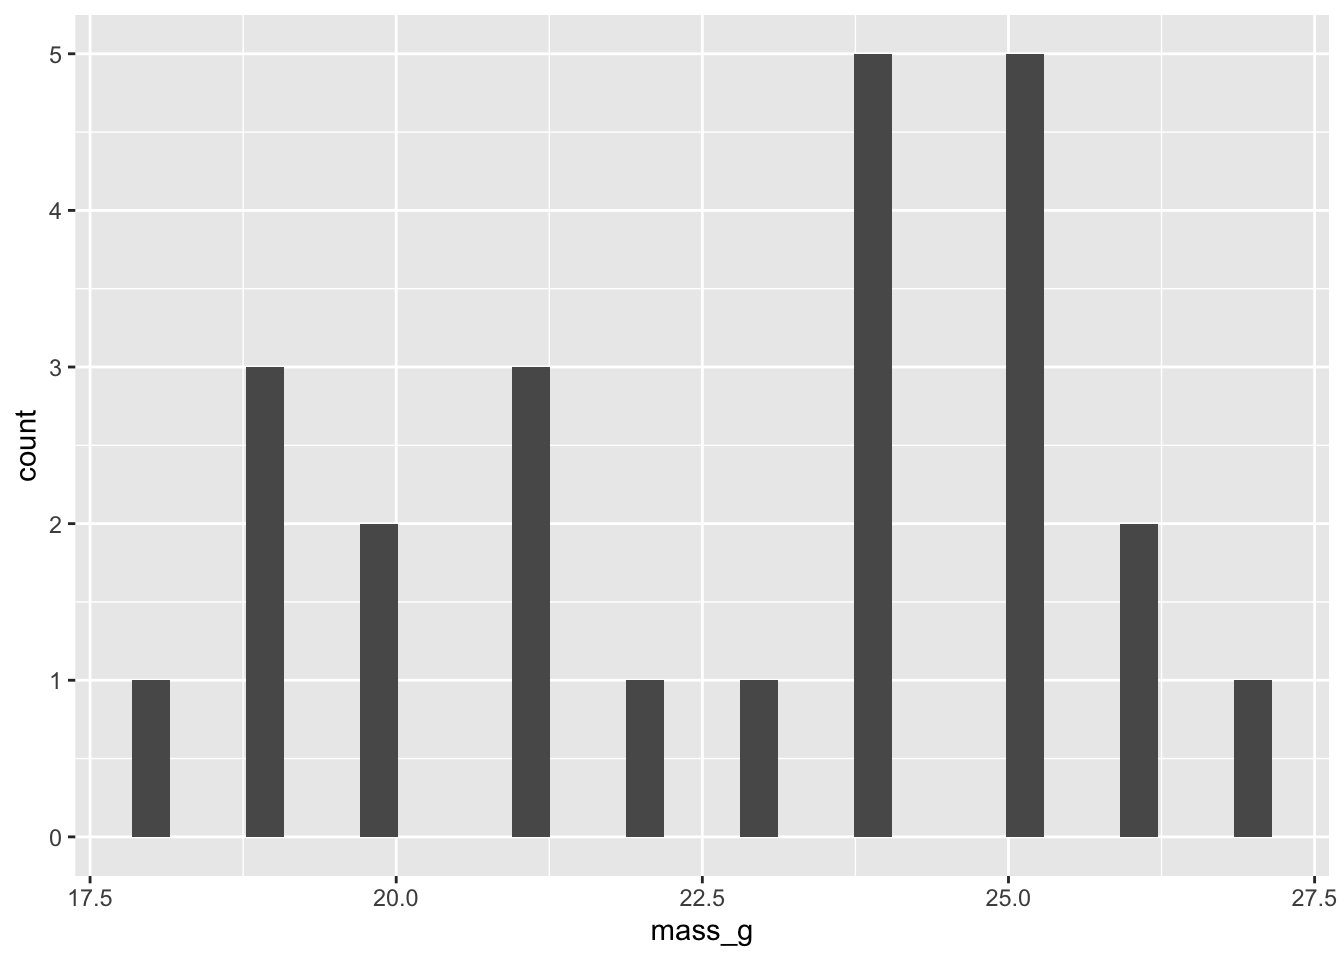
\includegraphics{r_visualize_files/figure-pdf/unnamed-chunk-3-1.pdf}

There, a simple histogram. Now let's play with how it looks:

\begin{Shaded}
\begin{Highlighting}[]
\DocumentationTok{\#\# make a ggplot, use wf\_mice data, and specify mass as the x variable}
\FunctionTok{ggplot}\NormalTok{(}\AttributeTok{data =}\NormalTok{ wf\_mice, }\FunctionTok{aes}\NormalTok{(}\AttributeTok{x =}\NormalTok{ mass\_g)) }\SpecialCharTok{+}
  \DocumentationTok{\#\# give a wider binwidth to the histogram, and make it grey bars with black outlines}
  \FunctionTok{geom\_histogram}\NormalTok{(}\AttributeTok{binwidth =} \DecValTok{1}\NormalTok{, }\AttributeTok{fill =} \StringTok{"grey"}\NormalTok{, }\AttributeTok{color =} \StringTok{"black"}\NormalTok{) }\SpecialCharTok{+} 
  \FunctionTok{labs}\NormalTok{(}\AttributeTok{x =} \StringTok{"White{-}footed Mouse Mass (g)"}\NormalTok{, }\AttributeTok{y =} \StringTok{"Count"}\NormalTok{) }\SpecialCharTok{+} \DocumentationTok{\#\# nicer labels}
  \FunctionTok{theme\_bw}\NormalTok{() }\DocumentationTok{\#\# my favorite simple theme}
\end{Highlighting}
\end{Shaded}

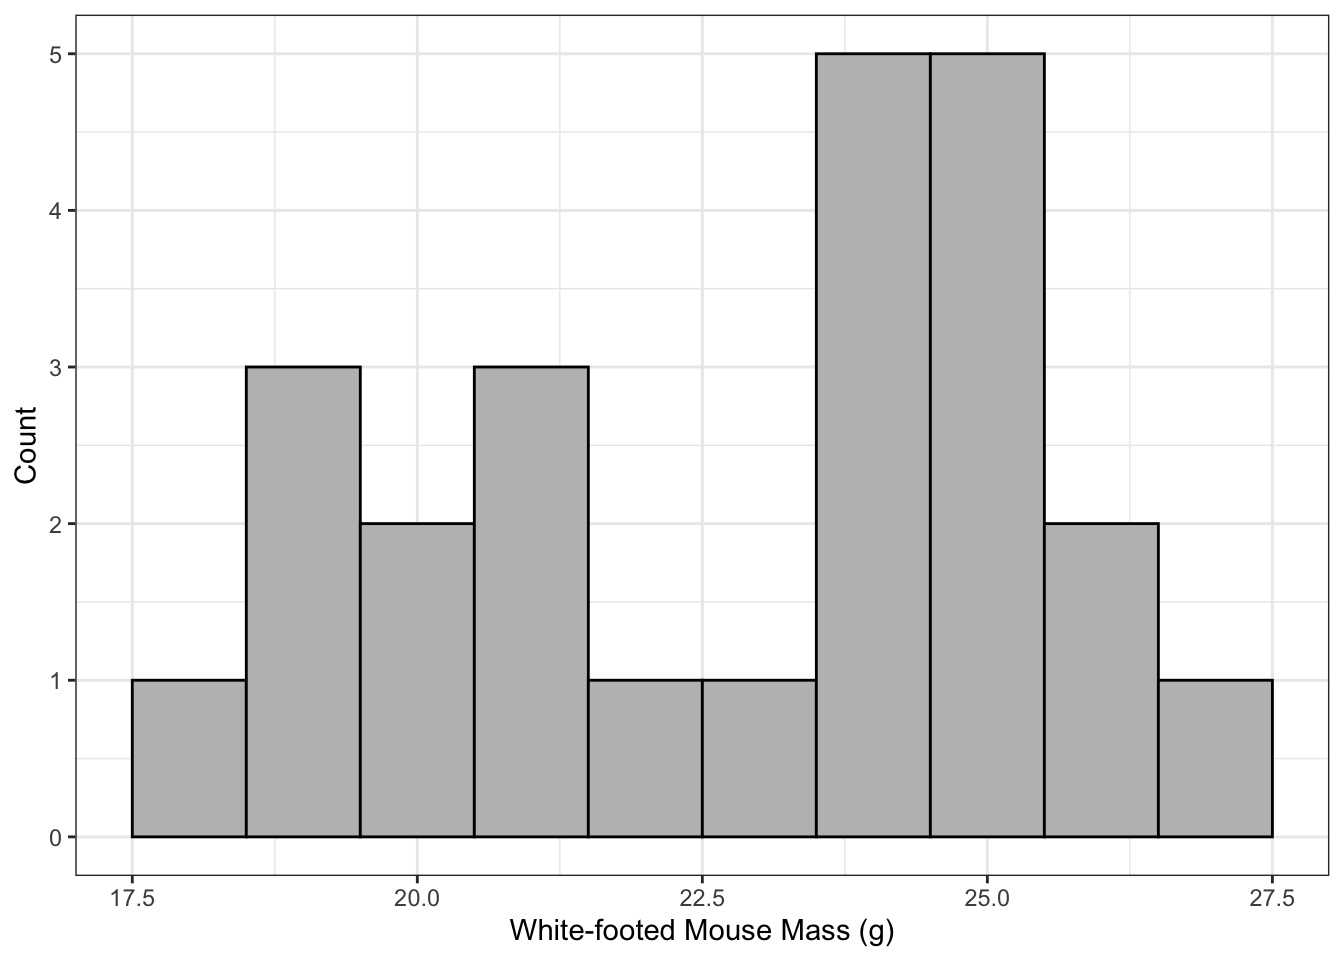
\includegraphics{r_visualize_files/figure-pdf/unnamed-chunk-4-1.pdf}

Cool! We could also look at this as a density plot! This will give more
of a smooth line

\begin{Shaded}
\begin{Highlighting}[]
\DocumentationTok{\#\# make a ggplot, use wf\_mice data, and specify mass as the x variable}
\FunctionTok{ggplot}\NormalTok{(}\AttributeTok{data =}\NormalTok{ wf\_mice, }\FunctionTok{aes}\NormalTok{(}\AttributeTok{x =}\NormalTok{ mass\_g)) }\SpecialCharTok{+}
  \FunctionTok{geom\_density}\NormalTok{() }\SpecialCharTok{+} \DocumentationTok{\#\# create density plot}
  \FunctionTok{labs}\NormalTok{(}\AttributeTok{x =} \StringTok{"White{-}footed Mouse Mass (g)"}\NormalTok{, }\AttributeTok{y =} \StringTok{"Frequency"}\NormalTok{) }\SpecialCharTok{+} \DocumentationTok{\#\# nicer labels}
  \FunctionTok{theme\_bw}\NormalTok{() }\DocumentationTok{\#\# my favorite simple theme}
\end{Highlighting}
\end{Shaded}

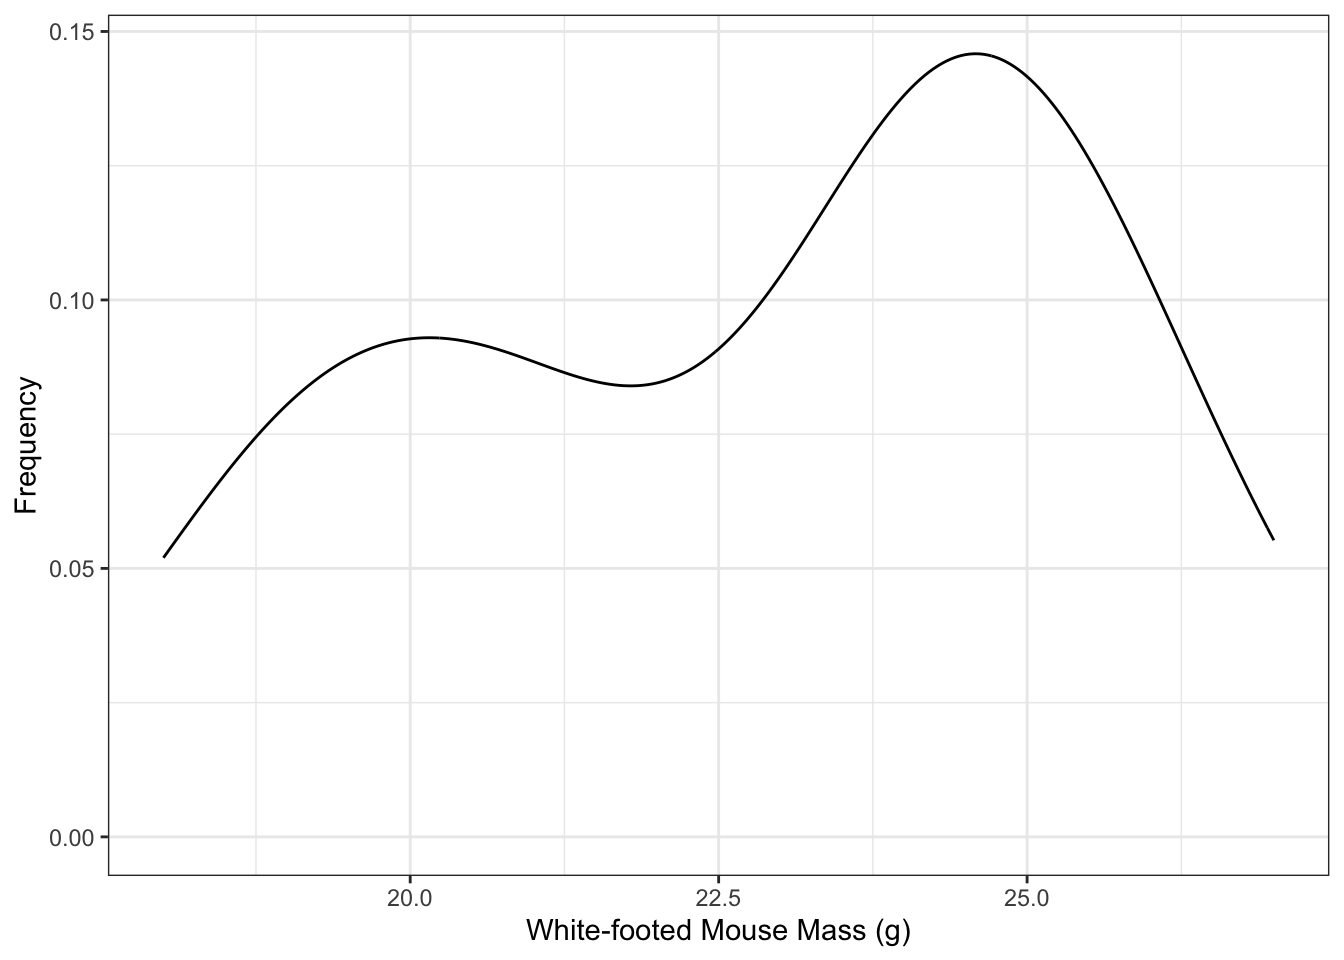
\includegraphics{r_visualize_files/figure-pdf/unnamed-chunk-5-1.pdf}

\subsection{One Variable: Categorical}\label{one-variable-categorical}

If you want to show how many observations are in each category, you can
use a bar plot.

In this demo, let's make a bar plot of how many of each mammal species
were caught.

\begin{Shaded}
\begin{Highlighting}[]
\DocumentationTok{\#\# specify x as species}
\FunctionTok{ggplot}\NormalTok{(}\AttributeTok{data =}\NormalTok{ fake\_mammals, }\FunctionTok{aes}\NormalTok{(}\AttributeTok{x =}\NormalTok{ species)) }\SpecialCharTok{+}
  \FunctionTok{geom\_bar}\NormalTok{() }\DocumentationTok{\#\# make bar plot}
\end{Highlighting}
\end{Shaded}

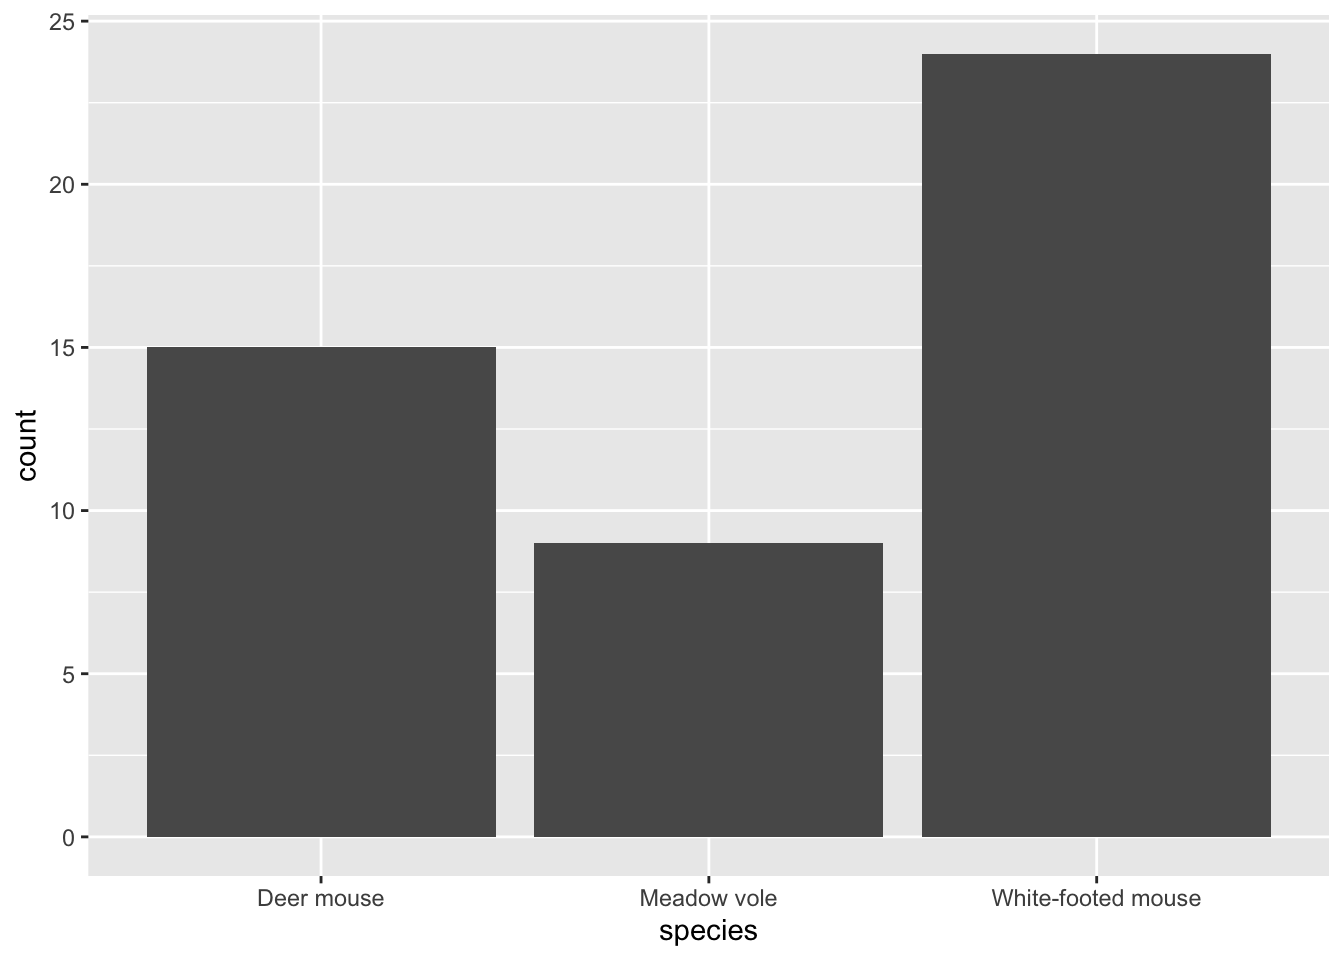
\includegraphics{r_visualize_files/figure-pdf/unnamed-chunk-6-1.pdf}

The geom\_bar function will count up all the observations of each
species level to inform its bars. Thus, it is assuming you are giving it
long data. Another closely related function is geom\_col, which just
makes a bar as tall as a number value in the data. For example, let's
make a bar plot of how many insect were caught at each site.

\begin{Shaded}
\begin{Highlighting}[]
\DocumentationTok{\#\# need to specify two variables this time, one for the category, one for the count value}
\FunctionTok{ggplot}\NormalTok{(}\AttributeTok{data =}\NormalTok{ insect\_counts, }\FunctionTok{aes}\NormalTok{(}\AttributeTok{x =}\NormalTok{ site, }\AttributeTok{y =}\NormalTok{ total\_insects)) }\SpecialCharTok{+}
  \FunctionTok{geom\_col}\NormalTok{()}
\end{Highlighting}
\end{Shaded}

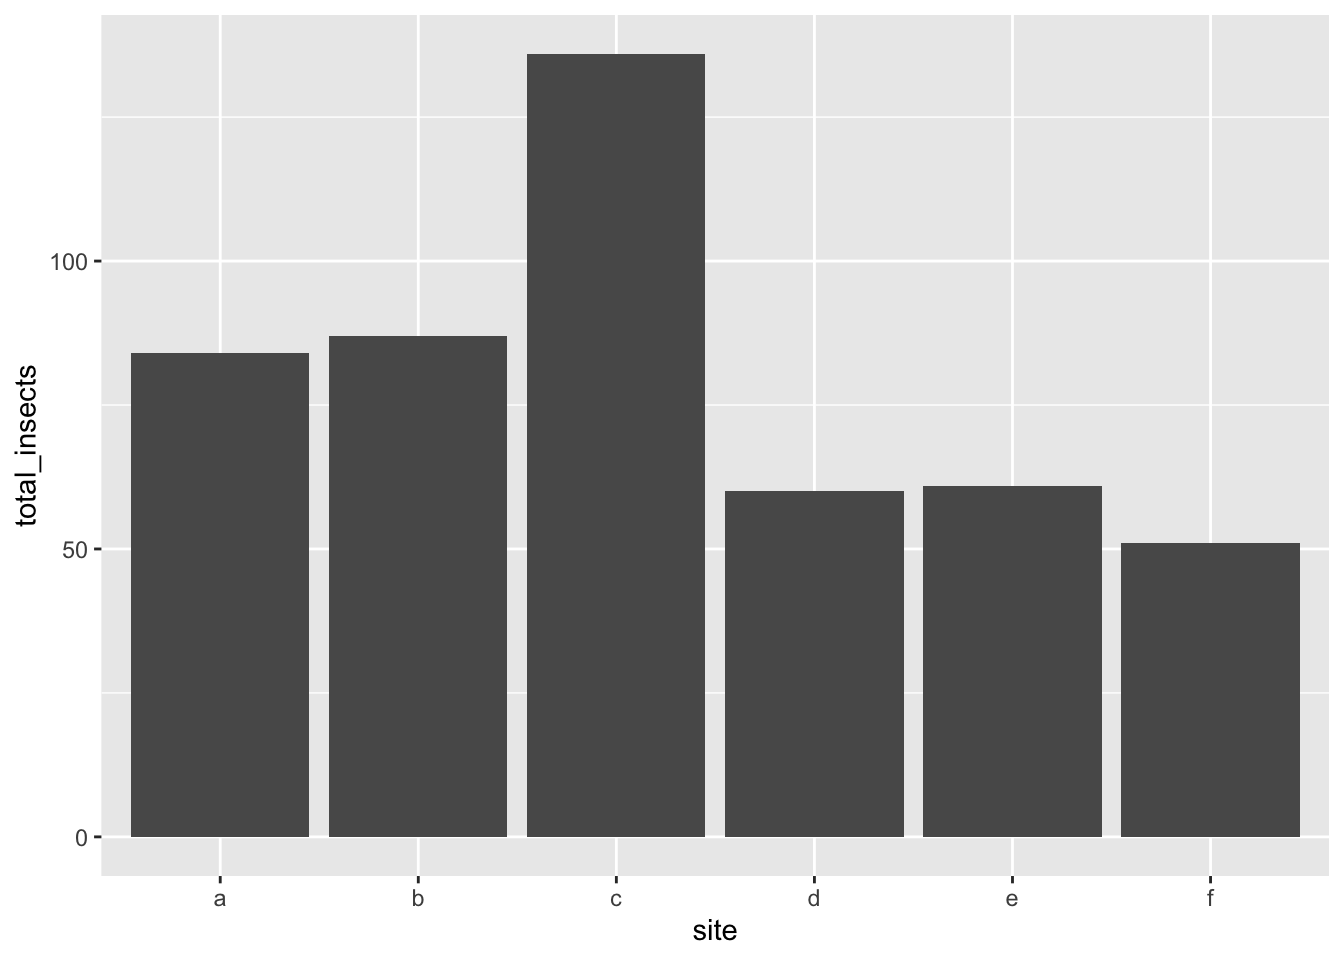
\includegraphics{r_visualize_files/figure-pdf/unnamed-chunk-7-1.pdf}

As you can see, your data format will determine whether you should use
geom\_col or geom\_bar. Note: bar plots are generally only best-suited
for counts among categories, when you're dealing with measured
variables, there are better options below.

\subsection{Two Variables: Both
Continuous}\label{two-variables-both-continuous}

If you are showing the relationship between two continuous variables,
scatterplots with or without lines are usually the best way to go.

Let's try it out with the mammal data on body mass and helminth mass in
mice:

\begin{Shaded}
\begin{Highlighting}[]
\DocumentationTok{\#\# filter for mouse data}
\NormalTok{mouse\_data }\OtherTok{\textless{}{-}} \FunctionTok{filter}\NormalTok{(fake\_mammals, species }\SpecialCharTok{\%in\%} \FunctionTok{c}\NormalTok{(}\StringTok{"White{-}footed mouse"}\NormalTok{, }\StringTok{"Deer mouse"}\NormalTok{))}

\DocumentationTok{\#\# create ggplot with your two continuous variables as x and y}
\FunctionTok{ggplot}\NormalTok{(}\AttributeTok{data =}\NormalTok{ mouse\_data, }\FunctionTok{aes}\NormalTok{(}\AttributeTok{x =}\NormalTok{ mass\_g, }\AttributeTok{y =}\NormalTok{ helminth\_mass\_mg)) }\SpecialCharTok{+}
  \FunctionTok{geom\_point}\NormalTok{() }\DocumentationTok{\#\# create scatterplot}
\end{Highlighting}
\end{Shaded}

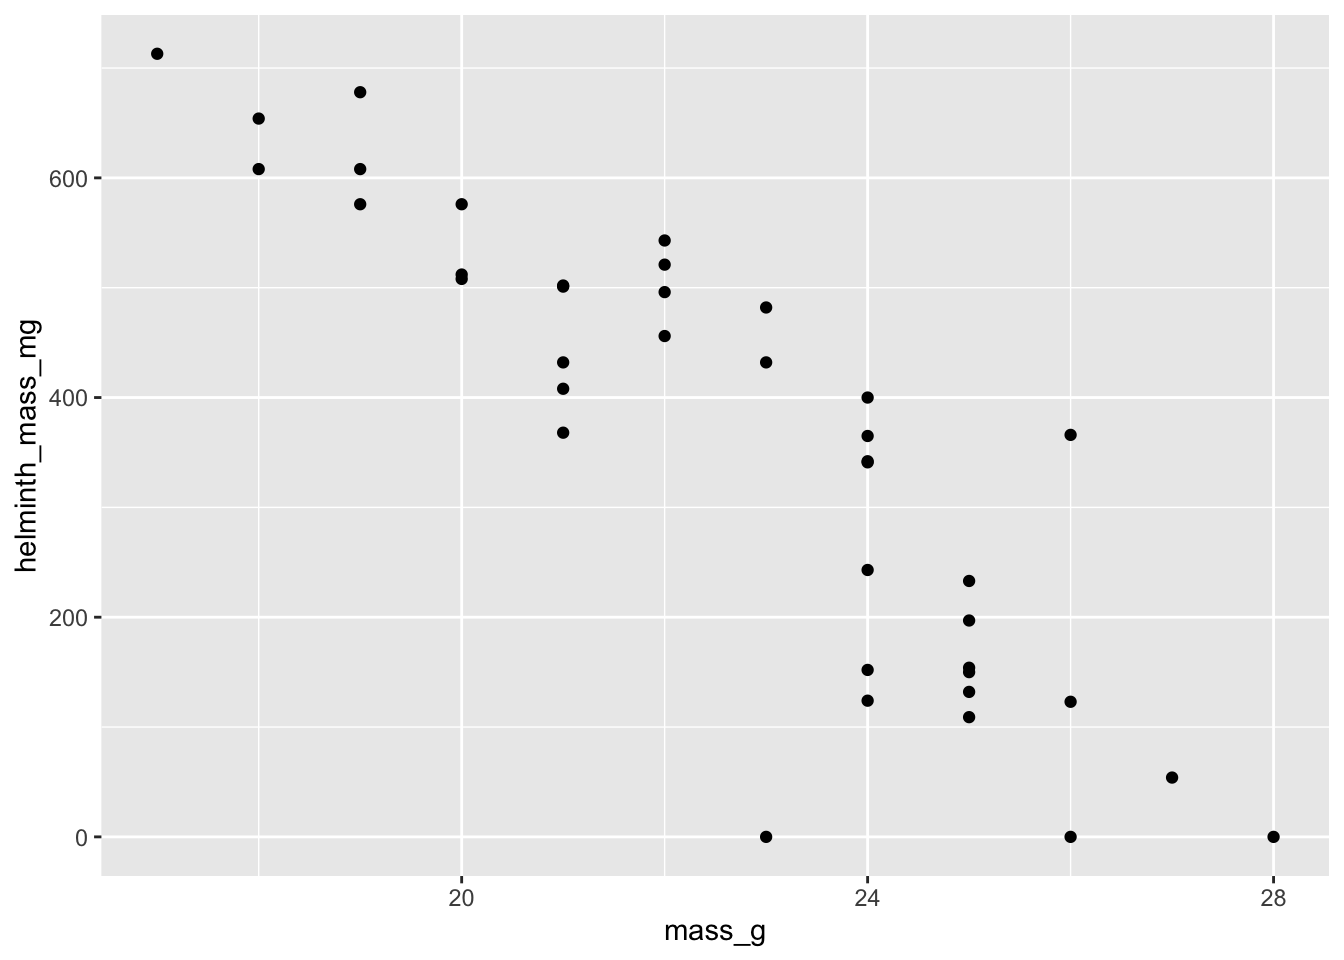
\includegraphics{r_visualize_files/figure-pdf/unnamed-chunk-8-1.pdf}

\begin{Shaded}
\begin{Highlighting}[]
\DocumentationTok{\#\# with trendline}
\FunctionTok{ggplot}\NormalTok{(}\AttributeTok{data =}\NormalTok{ mouse\_data, }\FunctionTok{aes}\NormalTok{(}\AttributeTok{x =}\NormalTok{ mass\_g, }\AttributeTok{y =}\NormalTok{ helminth\_mass\_mg)) }\SpecialCharTok{+}
  \FunctionTok{geom\_point}\NormalTok{() }\SpecialCharTok{+}  \DocumentationTok{\#\# create scatterplot}
  \DocumentationTok{\#\# create a trendline; method = "lm" makes it a straight line, se specifys whether there are error regions shaded}
  \FunctionTok{geom\_smooth}\NormalTok{(}\AttributeTok{method =} \StringTok{"lm"}\NormalTok{, }\AttributeTok{se =} \ConstantTok{FALSE}\NormalTok{)}
\end{Highlighting}
\end{Shaded}

\begin{verbatim}
`geom_smooth()` using formula = 'y ~ x'
\end{verbatim}

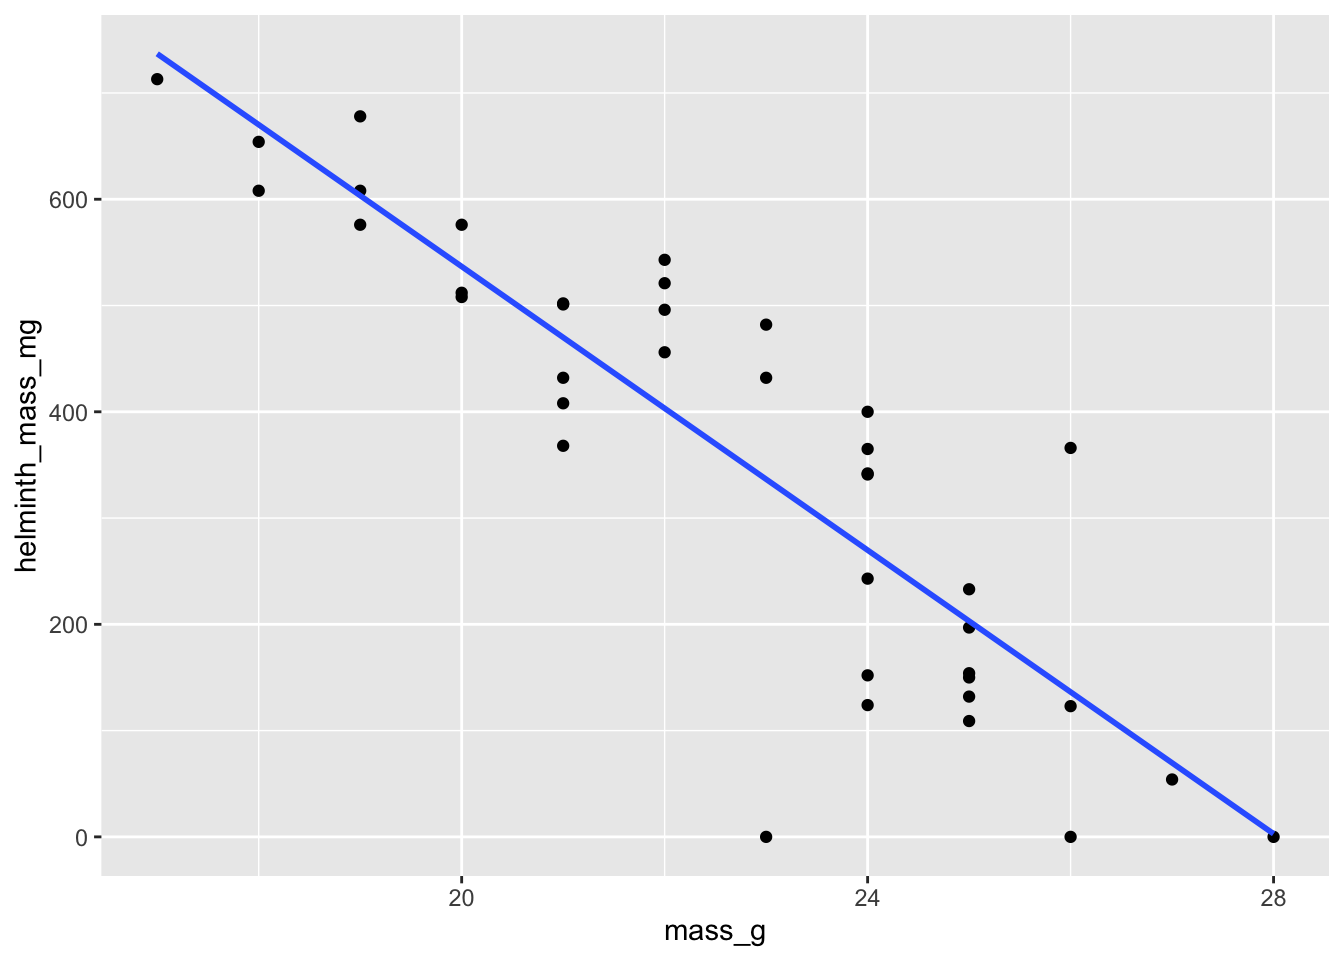
\includegraphics{r_visualize_files/figure-pdf/unnamed-chunk-8-2.pdf}

\subsection{Two Variables: One Continuous, One
Categorical}\label{two-variables-one-continuous-one-categorical}

Believe it or not, when one of your variables is categorical, a
scatterplot is still appropriate. Why not a bar plot? Because
scatterplots show all of your data!

Let's demonstrate with the mammal data by comparing helminth mass among
species.

\begin{Shaded}
\begin{Highlighting}[]
\DocumentationTok{\#\# create ggplot with your two variables as x and y}
\FunctionTok{ggplot}\NormalTok{(}\AttributeTok{data =}\NormalTok{ fake\_mammals, }\FunctionTok{aes}\NormalTok{(}\AttributeTok{x =}\NormalTok{ species, }\AttributeTok{y =}\NormalTok{ helminth\_mass\_mg)) }\SpecialCharTok{+}
  \FunctionTok{geom\_jitter}\NormalTok{(}\AttributeTok{width =} \FloatTok{0.1}\NormalTok{, }\AttributeTok{height =} \DecValTok{0}\NormalTok{) }\DocumentationTok{\#\# create points that are "jittered" a bit along the x axis}
\end{Highlighting}
\end{Shaded}

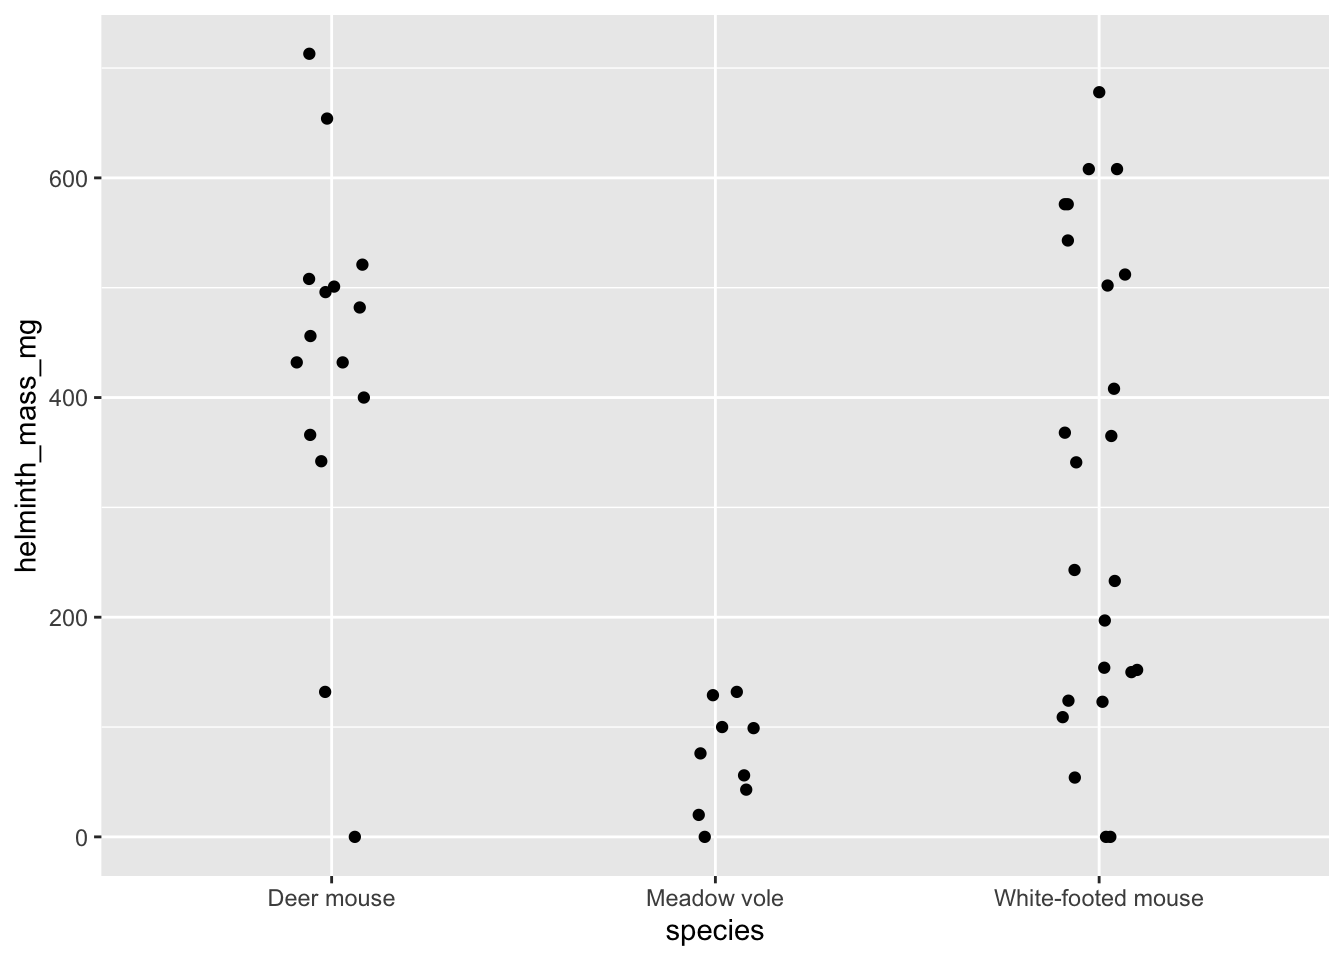
\includegraphics{r_visualize_files/figure-pdf/unnamed-chunk-9-1.pdf}

In this plot, we use geom\_jitter to make the point spread a bit around
each categorical X value so that you can see them better (but we specify
height = 0 so as not to mess with the mass information). Instead of a
mean helminth mass given by a bar plot, we can see the spread of each
set of datapoints, including outliers or lack thereof. Still it's often
nice to add some structure to these plots, which can be geom\_boxplot or
geom\_violin (among others). Here is an example:

\begin{Shaded}
\begin{Highlighting}[]
\DocumentationTok{\#\# create ggplot with your two variables as x and y}
\FunctionTok{ggplot}\NormalTok{(}\AttributeTok{data =}\NormalTok{ fake\_mammals, }\FunctionTok{aes}\NormalTok{(}\AttributeTok{x =}\NormalTok{ species, }\AttributeTok{y =}\NormalTok{ helminth\_mass\_mg)) }\SpecialCharTok{+}
  \FunctionTok{geom\_jitter}\NormalTok{(}\AttributeTok{width =} \FloatTok{0.1}\NormalTok{, }\AttributeTok{height =} \DecValTok{0}\NormalTok{) }\SpecialCharTok{+} \DocumentationTok{\#\# create points that are "jittered" a bit along the x axis}
  \FunctionTok{geom\_boxplot}\NormalTok{(}\AttributeTok{alpha =} \FloatTok{0.2}\NormalTok{) }\DocumentationTok{\#\# create boxplot at 20\% transparency with alpha}
\end{Highlighting}
\end{Shaded}

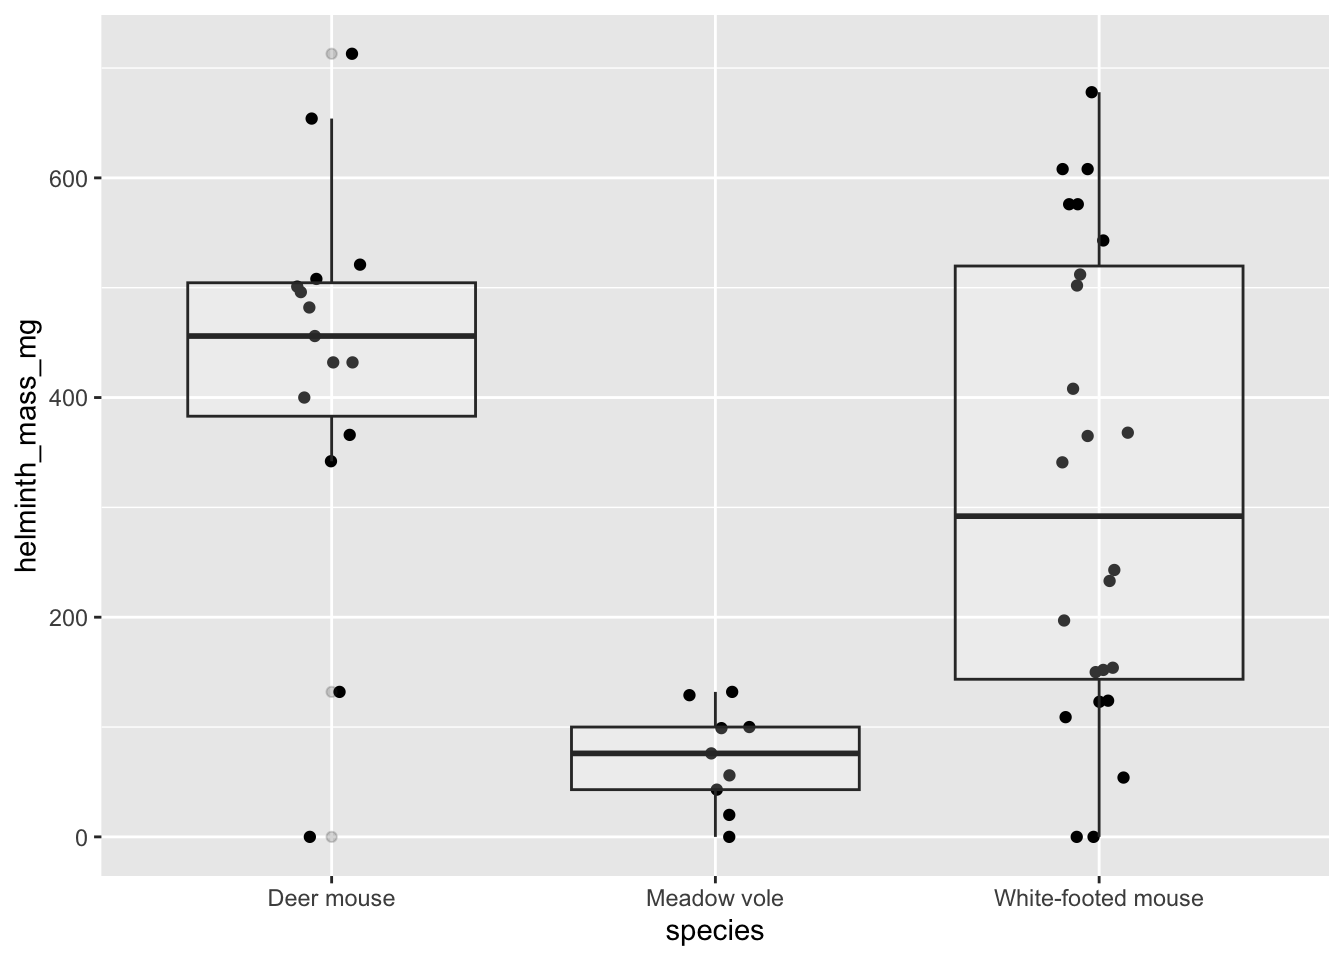
\includegraphics{r_visualize_files/figure-pdf/unnamed-chunk-10-1.pdf}

We could also make this plot even clearer by adding color:

\begin{Shaded}
\begin{Highlighting}[]
\DocumentationTok{\#\# create ggplot with your two variables as x and y}
\FunctionTok{ggplot}\NormalTok{(}\AttributeTok{data =}\NormalTok{ fake\_mammals, }\FunctionTok{aes}\NormalTok{(}\AttributeTok{x =}\NormalTok{ species, }\AttributeTok{y =}\NormalTok{ helminth\_mass\_mg)) }\SpecialCharTok{+}
  \FunctionTok{geom\_jitter}\NormalTok{(}\FunctionTok{aes}\NormalTok{(}\AttributeTok{color =}\NormalTok{ species), }\AttributeTok{width =} \FloatTok{0.1}\NormalTok{, }\AttributeTok{height =} \DecValTok{0}\NormalTok{) }\SpecialCharTok{+} \DocumentationTok{\#\# you can put aes() inside geoms}
  \FunctionTok{geom\_boxplot}\NormalTok{(}\FunctionTok{aes}\NormalTok{(}\AttributeTok{fill =}\NormalTok{ species), }\AttributeTok{alpha =} \FloatTok{0.2}\NormalTok{) }\SpecialCharTok{+}
  \FunctionTok{labs}\NormalTok{(}\AttributeTok{x =} \StringTok{"Species"}\NormalTok{, }\AttributeTok{y =} \StringTok{"Helminth Mass (mg)"}\NormalTok{) }\SpecialCharTok{+}
  \FunctionTok{theme\_bw}\NormalTok{() }\SpecialCharTok{+}
  \FunctionTok{theme}\NormalTok{(}\AttributeTok{legend.position =} \StringTok{"none"}\NormalTok{) }\DocumentationTok{\#\# legend is redundant here, so we can hide it}
\end{Highlighting}
\end{Shaded}

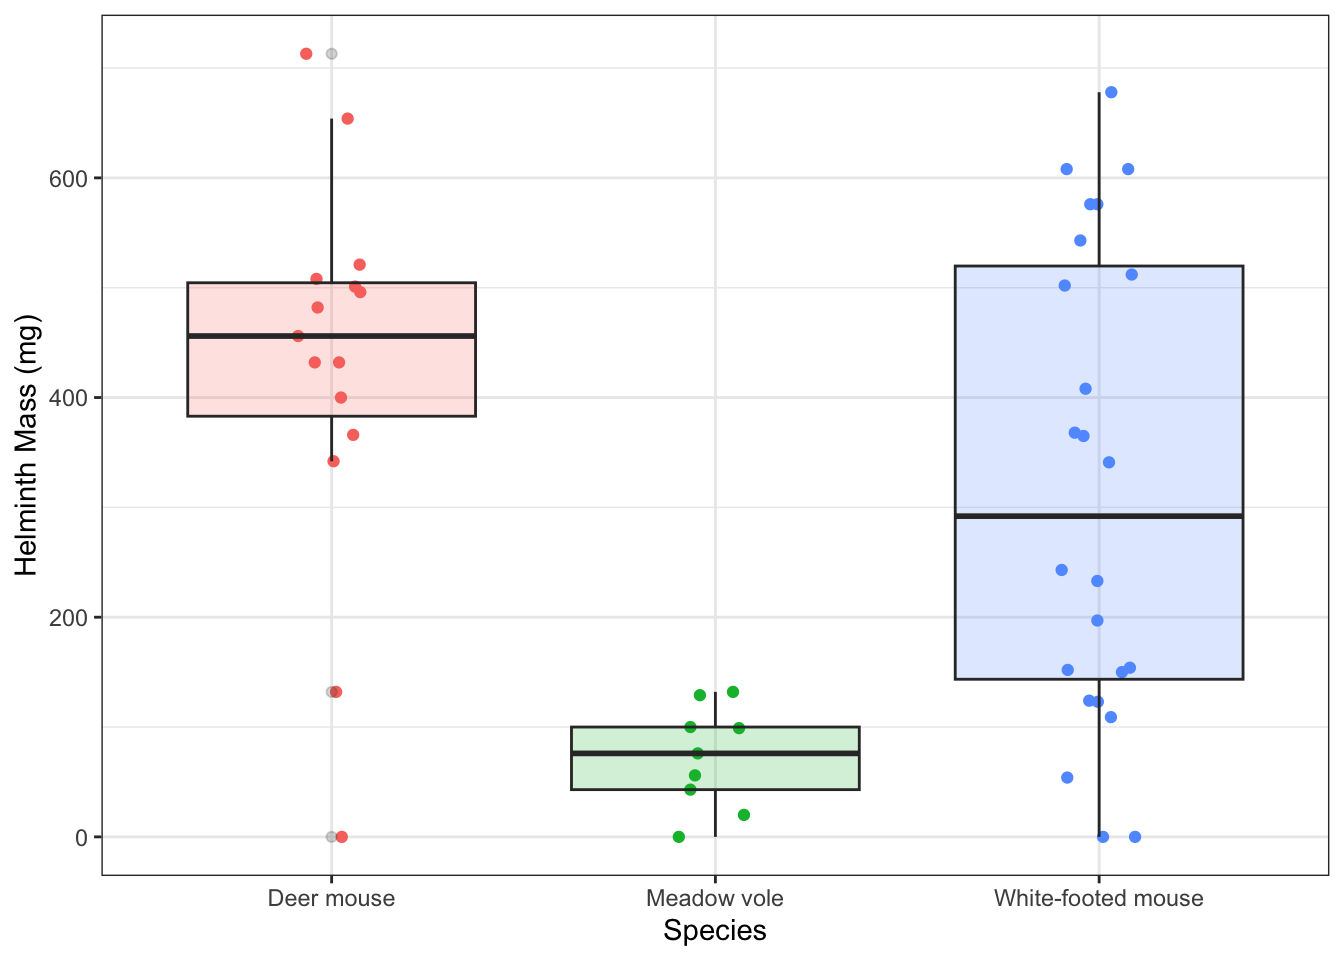
\includegraphics{r_visualize_files/figure-pdf/unnamed-chunk-11-1.pdf}

\subsection{Non-Axis Variables}\label{non-axis-variables}

You can also use other aesthetics to represent variables in your data.
For example, you could use color to show the density plots of mammal
masses among species. And you can modify the colors with scale
functions:

\begin{Shaded}
\begin{Highlighting}[]
\DocumentationTok{\#\# make a ggplot, use wf\_mice data, specify mass as the x variable and species as color}
\FunctionTok{ggplot}\NormalTok{(}\AttributeTok{data =}\NormalTok{ fake\_mammals, }\FunctionTok{aes}\NormalTok{(}\AttributeTok{x =}\NormalTok{ mass\_g, }\AttributeTok{color =}\NormalTok{ species)) }\SpecialCharTok{+}
  \FunctionTok{geom\_density}\NormalTok{() }\SpecialCharTok{+} \DocumentationTok{\#\# create density plot}
  \FunctionTok{scale\_color\_manual}\NormalTok{(}\AttributeTok{values =} \FunctionTok{c}\NormalTok{(}\StringTok{"red"}\NormalTok{, }\StringTok{"blue"}\NormalTok{, }\StringTok{"green"}\NormalTok{)) }\SpecialCharTok{+} \DocumentationTok{\#\# set my own colors}
  \FunctionTok{labs}\NormalTok{(}\AttributeTok{x =} \StringTok{"Mammal Mass (g)"}\NormalTok{, }\AttributeTok{y =} \StringTok{"Frequency"}\NormalTok{) }\SpecialCharTok{+} \DocumentationTok{\#\# nicer labels}
  \FunctionTok{theme\_bw}\NormalTok{() }\DocumentationTok{\#\# my favorite simple theme}
\end{Highlighting}
\end{Shaded}

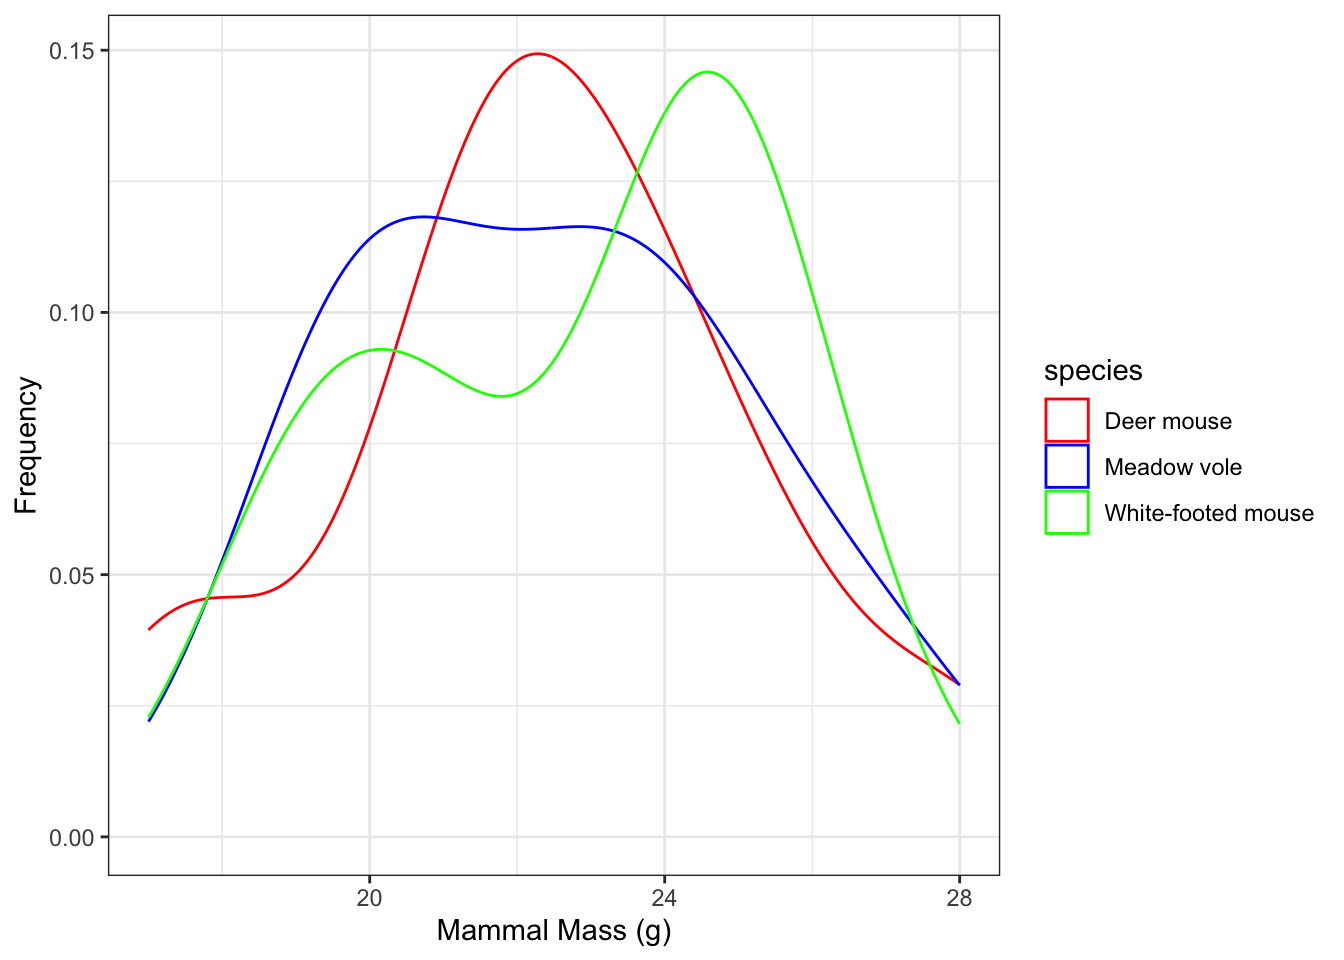
\includegraphics{r_visualize_files/figure-pdf/unnamed-chunk-12-1.pdf}

Similarly, you can add a third variable to a two variable figure. Take
the helminth mass by mammal body mass figure from above:

\begin{Shaded}
\begin{Highlighting}[]
\FunctionTok{ggplot}\NormalTok{(}\AttributeTok{data =}\NormalTok{ mouse\_data, }\FunctionTok{aes}\NormalTok{(}\AttributeTok{x =}\NormalTok{ mass\_g, }\AttributeTok{y =}\NormalTok{ helminth\_mass\_mg, }\AttributeTok{color =}\NormalTok{ species)) }\SpecialCharTok{+}
  \FunctionTok{geom\_point}\NormalTok{() }\SpecialCharTok{+}  \DocumentationTok{\#\# create scatterplot}
  \FunctionTok{geom\_smooth}\NormalTok{(}\AttributeTok{method =} \StringTok{"lm"}\NormalTok{, }\AttributeTok{se =} \ConstantTok{FALSE}\NormalTok{)}
\end{Highlighting}
\end{Shaded}

\begin{verbatim}
`geom_smooth()` using formula = 'y ~ x'
\end{verbatim}

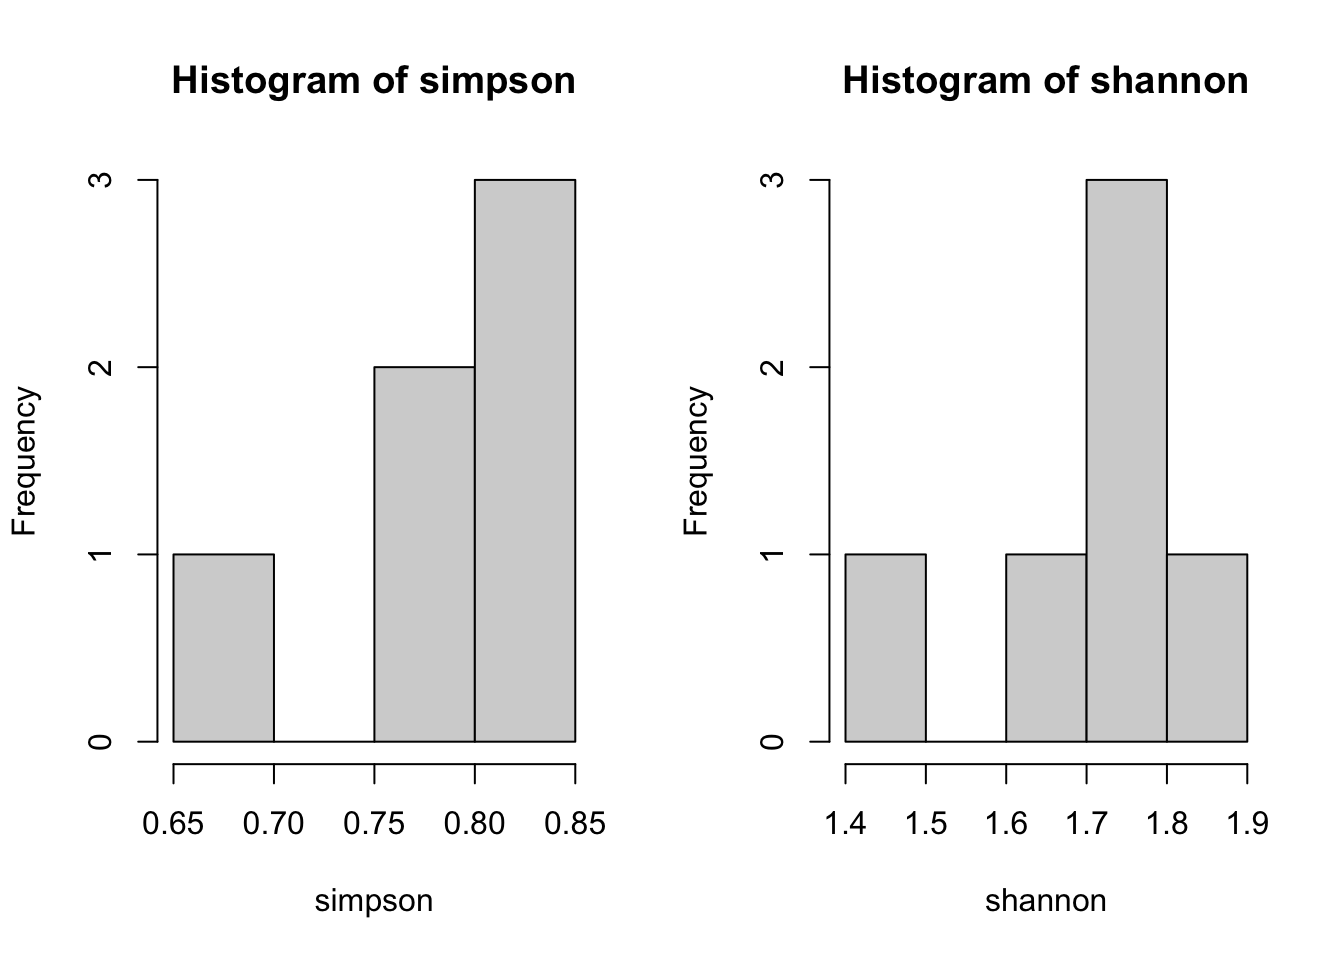
\includegraphics{r_visualize_files/figure-pdf/unnamed-chunk-13-1.pdf}

Color isn't the only way to show variables outside of axes, you can also
use point shape, size, linetype, etc. In addition, you can split data
among plot panels or ``facets'', with facet\_wrap() or facet\_grid().

Let's demonstrate with the long insect data, showing the insect
communities for each site:

\begin{Shaded}
\begin{Highlighting}[]
\DocumentationTok{\#\# specify order as y variable to show labels better}
\FunctionTok{ggplot}\NormalTok{(}\AttributeTok{data =}\NormalTok{ long\_insects, }\FunctionTok{aes}\NormalTok{(}\AttributeTok{y =}\NormalTok{ order, }\AttributeTok{x =}\NormalTok{ count, }\AttributeTok{fill =}\NormalTok{ site\_type)) }\SpecialCharTok{+}
  \FunctionTok{geom\_col}\NormalTok{() }\SpecialCharTok{+}
  \FunctionTok{facet\_wrap}\NormalTok{(}\FunctionTok{vars}\NormalTok{(site), }\AttributeTok{nrow =} \DecValTok{2}\NormalTok{) }\SpecialCharTok{+} \DocumentationTok{\#\# specify site variable, two rows to separate habitats}
  \FunctionTok{theme\_bw}\NormalTok{()}
\end{Highlighting}
\end{Shaded}

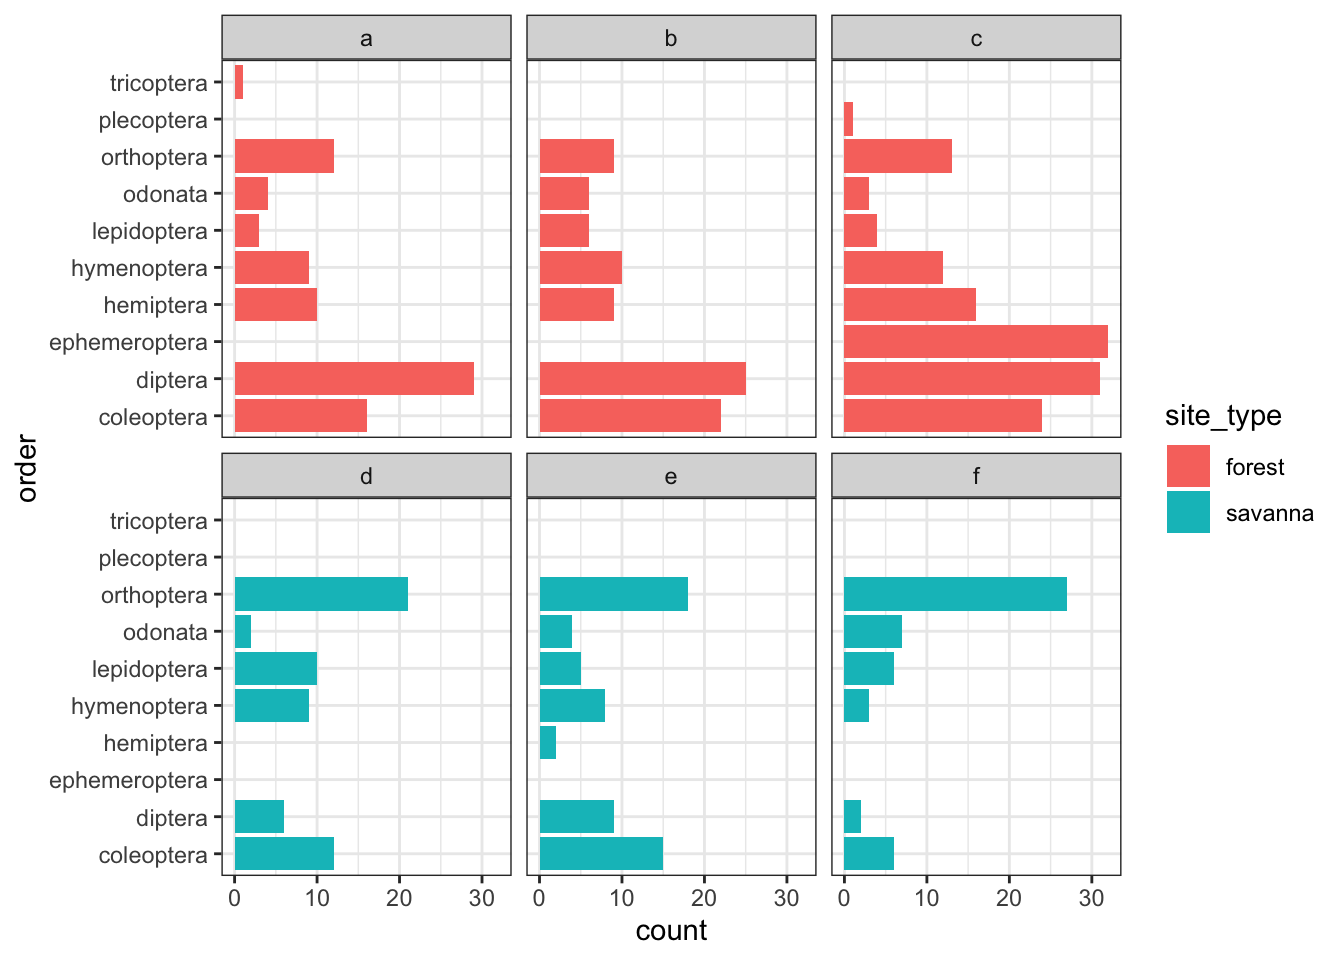
\includegraphics{r_visualize_files/figure-pdf/unnamed-chunk-14-1.pdf}

\subsection{Colorblind Safe Colors}\label{colorblind-safe-colors}

ggplot2 has colorblind-safe color schemes available from the
tidyverse-related package viridis.

For example:

\begin{Shaded}
\begin{Highlighting}[]
\DocumentationTok{\#\# make a ggplot, use wf\_mice data, specify mass as the x variable and species as color}
\FunctionTok{ggplot}\NormalTok{(}\AttributeTok{data =}\NormalTok{ fake\_mammals, }\FunctionTok{aes}\NormalTok{(}\AttributeTok{x =}\NormalTok{ mass\_g, }\AttributeTok{color =}\NormalTok{ species)) }\SpecialCharTok{+}
  \FunctionTok{geom\_density}\NormalTok{(}\AttributeTok{linewidth =} \DecValTok{1}\NormalTok{) }\SpecialCharTok{+} \DocumentationTok{\#\# create density plot, wider lines}
  \FunctionTok{scale\_color\_viridis\_d}\NormalTok{() }\SpecialCharTok{+} \DocumentationTok{\#\# set viridis discrete colors}
  \FunctionTok{labs}\NormalTok{(}\AttributeTok{x =} \StringTok{"Mammal Mass (g)"}\NormalTok{, }\AttributeTok{y =} \StringTok{"Frequency"}\NormalTok{) }\SpecialCharTok{+} \DocumentationTok{\#\# nicer labels}
  \FunctionTok{theme\_bw}\NormalTok{() }\DocumentationTok{\#\# my favorite simple theme}
\end{Highlighting}
\end{Shaded}

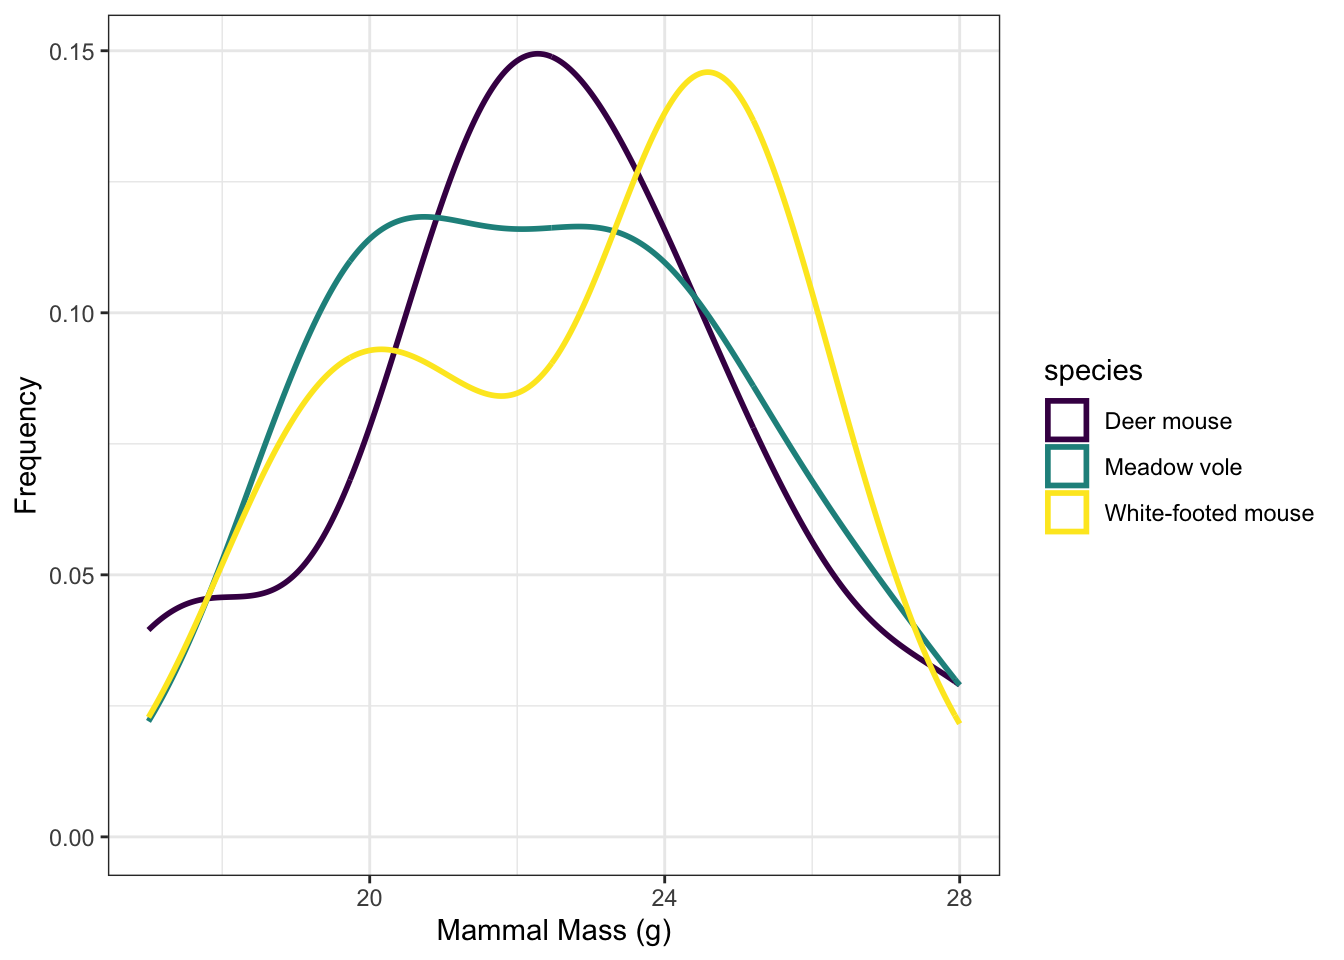
\includegraphics{r_visualize_files/figure-pdf/unnamed-chunk-15-1.pdf}

See the following link for more info:

\url{https://cran.r-project.org/web/packages/viridis/vignettes/intro-to-viridis.html}

\section{Further Reading}\label{further-reading}

We have only scratched the surface of what ggplot2 can do! We barely
discussed how to edit theme elements, nor did we spend much time on
customizing scales.

ggplot2 has an excellent reference website which you can find here:

\url{https://ggplot2.tidyverse.org/reference/index.html}

With it you can learn all the ins and outs!

\part{Appendices}

\chapter{Appendix A: More R
Resources}\label{appendix-a-more-r-resources}

Here is a collection of links to other useful resources for learning R!

Ecology-themed tutorial:

\url{https://datacarpentry.org/R-ecology-lesson/index.html}

\ul{Basic / Base R Materials}

Official R manuals:

\url{https://cran.r-project.org/manuals.html}

Cookbook for R (features lots of ``recipes'' for common tasks)

\url{http://www.cookbook-r.com/}

\ul{Primers and Cheatsheets (``tidyverse''-based)}

RStudio primers

\url{https://rstudio.cloud/learn/primers}

Tidyverse cheatsheets

\url{https://www.rstudio.com/resources/cheatsheets/}

\ul{Full Books and Courses}

Hadley Wickham's ``R for Data Science''

\url{https://r4ds.had.co.nz/index.html}

Hadley Wickham's ``Advanced R''

\url{https://adv-r.hadley.nz/}

Book for ``ggplot2'' package

\url{https://ggplot2-book.org/}

Jenny Bryan's STAT 545 course

\url{http://stat545.com/}

\ul{Package Function Reference Sites}

ggplot2 (data visualization)

\url{https://ggplot2.tidyverse.org/index.html}

sf (spatial analysis)

\url{https://r-spatial.github.io/sf/index.html}

\ul{Miscellaneous Resources}

On Style:

\url{http://adv-r.had.co.nz/Style.html}

On Reproducibility:

\url{https://reproducible-analysis-workshop.readthedocs.io/en/latest/}

\url{https://swcarpentry.github.io/r-novice-gapminder/}

\bookmarksetup{startatroot}

\chapter*{References}\label{references}
\addcontentsline{toc}{chapter}{References}

\markboth{References}{References}

\phantomsection\label{refs}
\begin{CSLReferences}{0}{1}
\end{CSLReferences}



\end{document}
